\documentclass{cup-pan}
\usepackage{blindtext}
\usepackage{comment}
\usepackage{setspace}
\usepackage{multicol}
\spacing{1.15}
\renewcommand*\contentsname{Summary of the contents}
\subsectionfont{\color{PANDarkBlue}}
\graphicspath{{Imagenes/}}

\title{Practical Coursework,\\ Video Game Fan Art, \\ The Legend of Zelda: Breath of the Wild.}

\author{Jesus Jimenez Montero}

\affil[1] {Informática Básica, VJ1202}
\affil[2] {Expresión Artística, VJ1204}
\affil[3] {Inglés Moderno, VJ1205}

%% Corresponding author
\corrauthor{Jesús Jiménez Montero}

%% Abbreviated author list for the running footer
\runningauthor{Jesus JM}

\addbibresource{refs.bib}

\begin{document}

\maketitle
%\hrule
\begin{figure}[H]
    
\includegraphics[width=\textwidth]{Imagenes/uanl (1).jpg}
\end{figure}
\textcolor{PANDarkBlue}{\hrule}

\medskip
%
%\begin{figure}[H]
%    \includegraphics[width=\textwidth]{Imagen de WhatsApp 2023-01-07 a las 23.%12.05.jpg}
%\end{figure}

\newpage
\tableofcontents
\newpage
\listoffigures
\newpage

\begin{abstract}
    This document is a practical coursework for the subject, “Informática Básica”. It's a fan art of the video game, “The Legend of Zelda: Breath of the Wild”. The main goal of this coursework is to adapt the Hero's Quest to the drawings.
    This document will be written in English due to the collaboration with the subject, “Inglés Moderno”. 
    And the format of the document is done with the language LaTeX, and the template PAN (Template for submission to Political Analysis).
\end{abstract}

%%______________________________________________________________________________
%%______________________________________________________________________________

\section{Introduction}

    \subsection{Description of the game}
    The Legend of Zelda, Breath of the Wild; is a video game exclusive to the Nintendo Switch console, released in 3rd March 2017. 
    Breath of the Wild is an open-world adventure game based on the world of Hyrule, 100 years after the battle that took place where Ganon was sealed in the castle of Hyrule with Zelda protecting the seal. Link is almost defeated on this battle and goes to a deep sleep.
    
    After 100 years as previously mentioned, he's woken up by a distant Zelda from its dormancy and goes out of the cave he was staying at, greeted by a distant and sinister Hyrule Castle. And the adventure can begin!\\
    
    \subsection{Adaptation of the hero's quest}
    One of the requirements for this coursework was to adapt the Hero's Quest to the drawings.
    To make my drawings accomplish this task, I used the key points of Link's Adventure, being:\\
        \begin{enumerate}
            \item After the extended tutorial where Link's gets its paraglider to get down the plateau where the game begins and one of the first things the player does is look to the Dueling Peaks, one of the key points on the game, where Link discovers its true quest.\\
            \item Where the player gains its confidence to destroy a Guardian, whose quest is to keep out intruders from key areas. This also a key point of the game because destroying a guardian means you are one step closer to defeating Ganon. \\
            \item The final cinematic of BOTW where Zelda talks to Link, telling him that his job is done, but there's a lot of to do\dots\\  \\
        \end{enumerate}

%%______________________________________________________________________________
%%______________________________________________________________________________
\newpage
\section{Reference images}

    For the images used in the project, I used a combination of images from the game (to make the fan arts as accurate as possible), images from internet and the most important par and 3D renders made in Blender.\\

    \subsection{Images from the game}
    Beginning with the captures of the game, for the Dueling Peaks, I used the following images:\\
        \begin{figure}[H]
            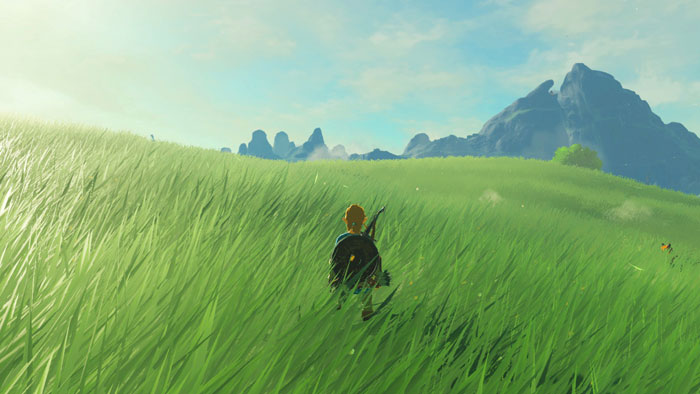
\includegraphics[width=\textwidth]{Imagenes/Referencias/article_img03_1.jpg}
            \caption{Image reference of the Dueling Peaks, with Link standing on a small grassy hill.}
        \end{figure}
    This image was used as a reference point on how the Dueling Peaks would look like when they were seen from a hill. 

    And this image: 
        \begin{figure}[H]
            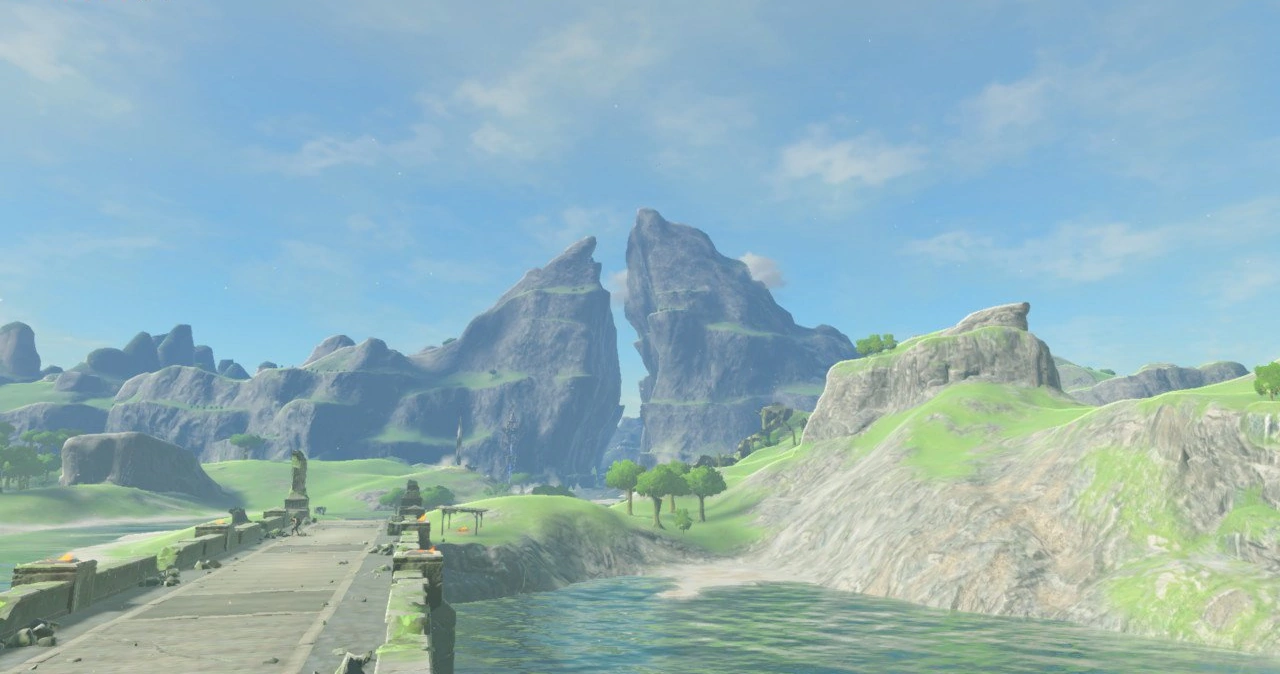
\includegraphics[width=\textwidth]{Imagenes/Referencias/Dueling_Peaks.png}
            \caption{The Dueling Peaks with the bridge near the enemy camp}
        \end{figure}
    Was used to see how the bridge that connected the path to the mountains looked like in the game.
    Also, because the bridge is over a river which connected with an enemy encampment. 

    \subsection{3D Renders}
    Before starting with this university career, I studied an Associate's Degree of Video Games, so I had previous expertise with using 3D rendering programs such as Blender, so I also used 3D renders to make some references for the fan arts, especially, for the character posing. \\

    So first, a simple blocks rig
        (\footnote{Rig made by 
        \href{https://hozq3d.gumroad.com/l/Blocks}{hozq3d}}) 
    was used to pose the character: 
    \begin{figure}[H]
        \includegraphics[width=\textwidth]{Imagenes/Referencias/renefernce_3d_3.png}
        \caption{Blocky character posing in an empty space, recreating the fan art.}
    \end{figure}

    After that, a rig of Zelda was used to pose the final character and create the character with much more detail:    
    (\footnote{Rig made by 
    \href{https://www.youtube.com/watch?v=1EUcGBMVRbA}{Soranin} and ported to Blender by  
    \href{https://twitter.com/mehaloArt/status/1528197222751383552?s=20}{mehaloArt}})

    \begin{figure}[H]
        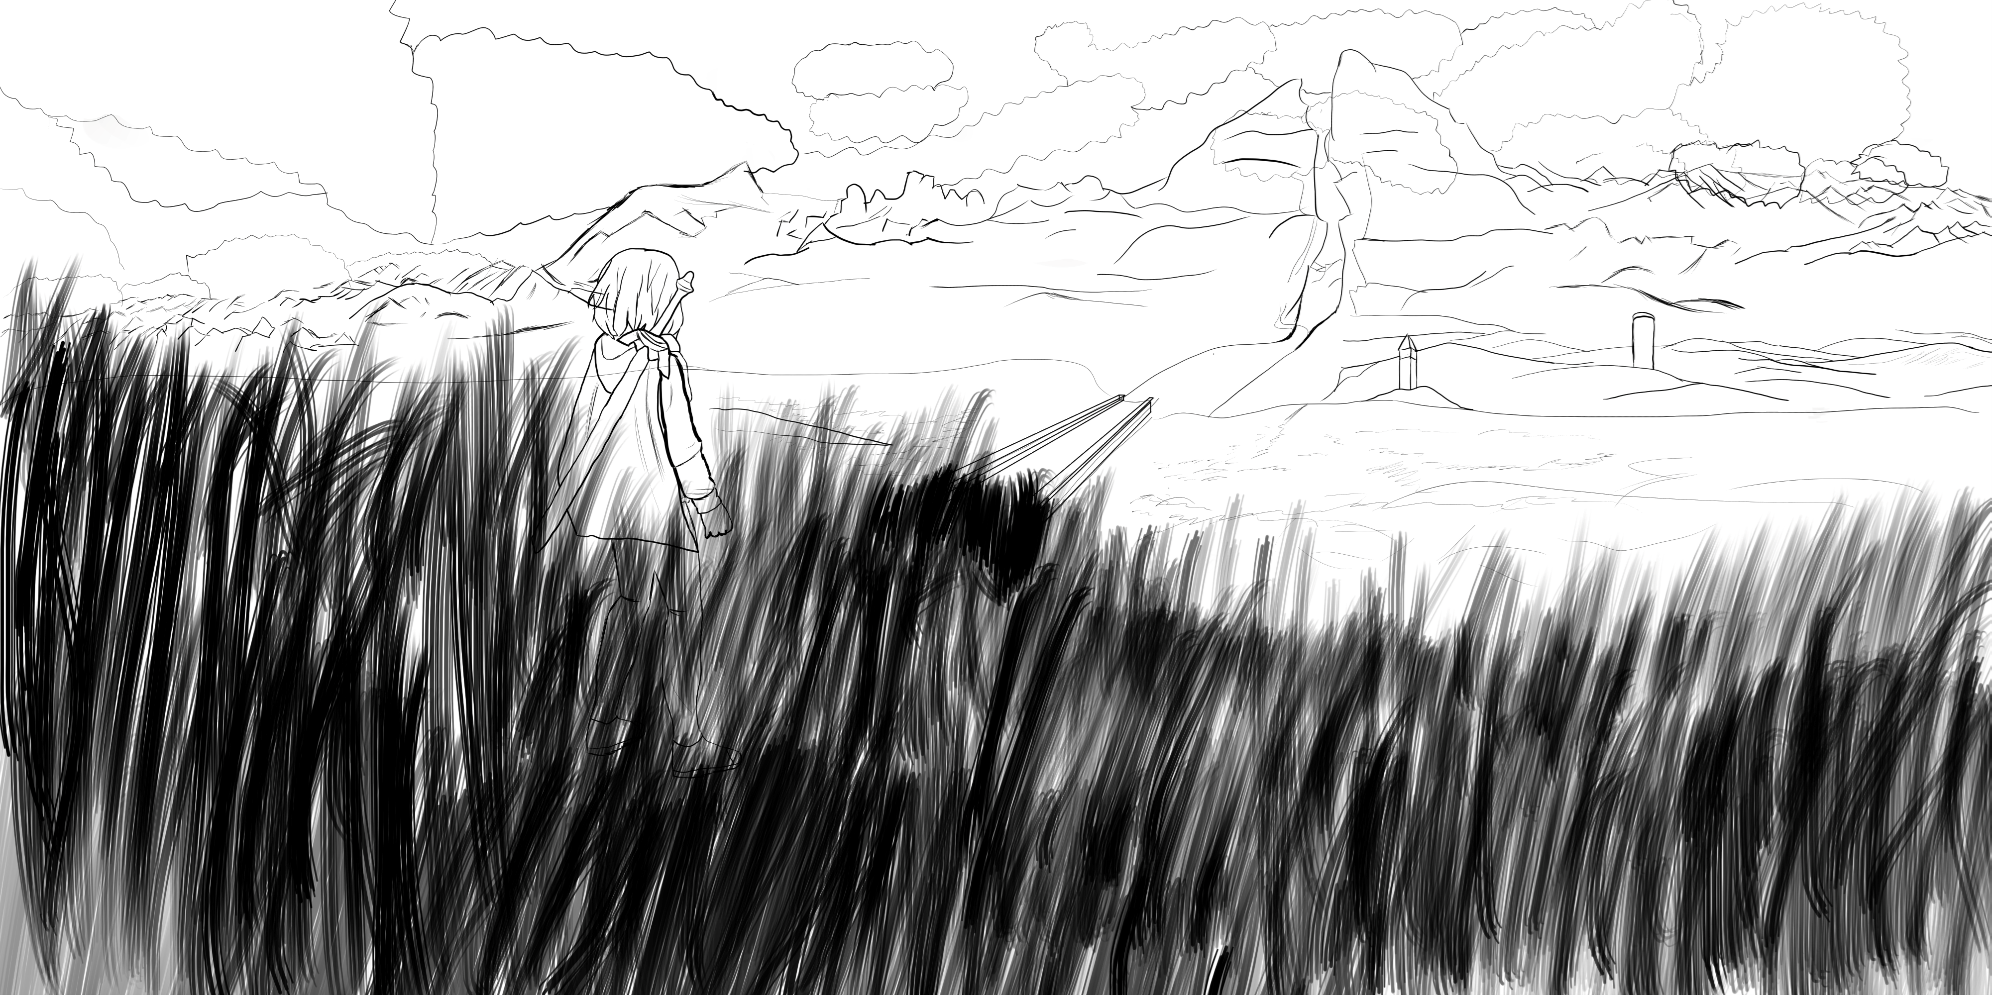
\includegraphics[width=\textwidth]{Imagenes/Referencias/ref_zelda.png}
        \caption{Picture of the line art with Zelda, using the rig mentioned.}
    \end{figure}

    The Zelda Rig was also used in combination with another rig, which was a Guardian 
    (\footnote{Rig made by 
        \href{https://sketchfab.com/3d-models/guardian-zelda-botw-fan-art-990a6a9434c849329360ea1ef9078895}{NinKorr3D}}), to make the final fan art.
    \begin{figure}[H]
        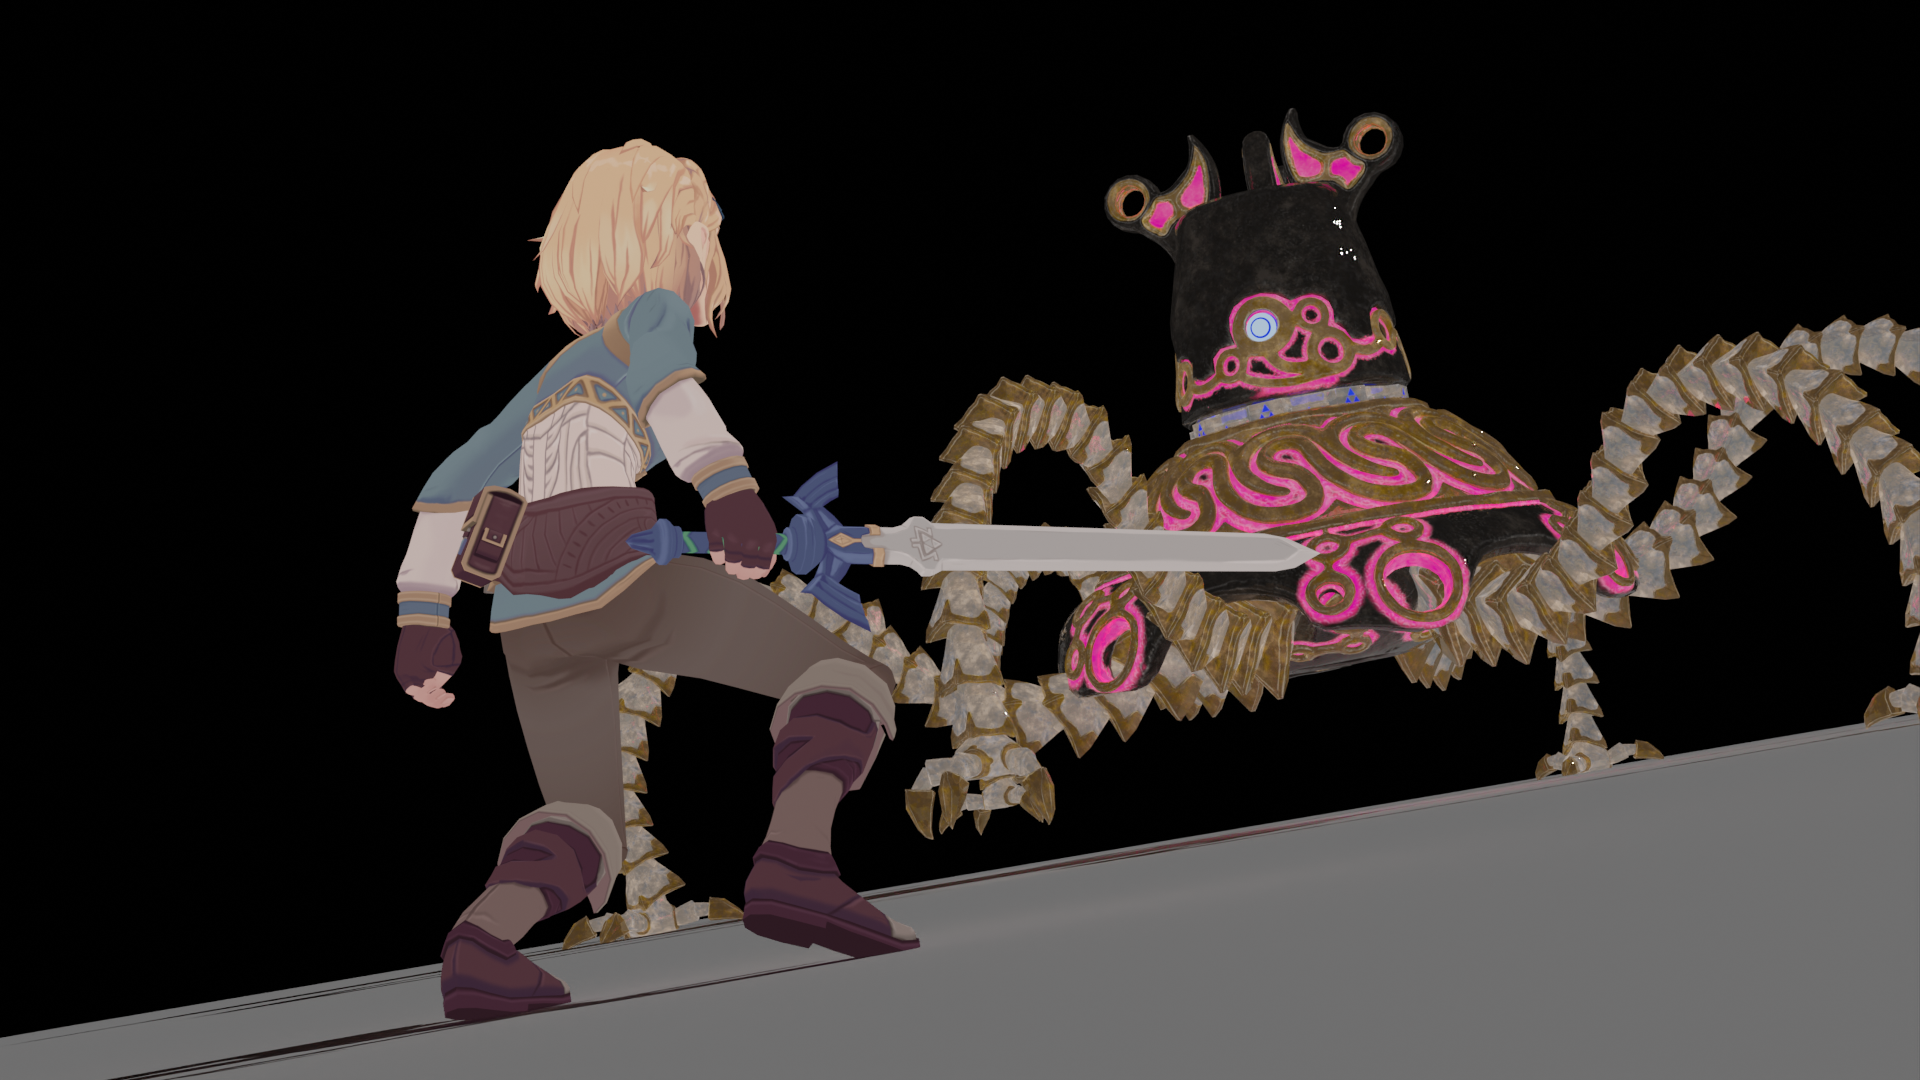
\includegraphics[width=\textwidth]{Imagenes/Referencias/referencia art 2.png}
        \caption{Zelda and Guardian Rig.}
    \end{figure}

    The usage of manually created 3D renders allowed for a much diverse expression of the fan arts, allowing a preview of how the final fan art would look like and facilitating the creation process.\\

    For the most part, the thematic of the fan arts was to create an impression on the spectator, make them feel something. For example, on the first fan art, I want the spectator to feel the same feeling that the player felt when it saw the Dueling Peaks for the first time. \\

    And on the second fan art, I want the spectator to feel the same feeling that the player has when it destroyed its first Guardian.

\newpage
%%______________________________________________________________________________
%%______________________________________________________________________________

\section{Analysis of formal elements of a concept art}

    This image a really early concept art released when BOTW was teased on 2017. I also selected it because it's really beautiful piece of art, but very \textit{“simple”} on its execution. 
    
    \begin{figure}[H]
       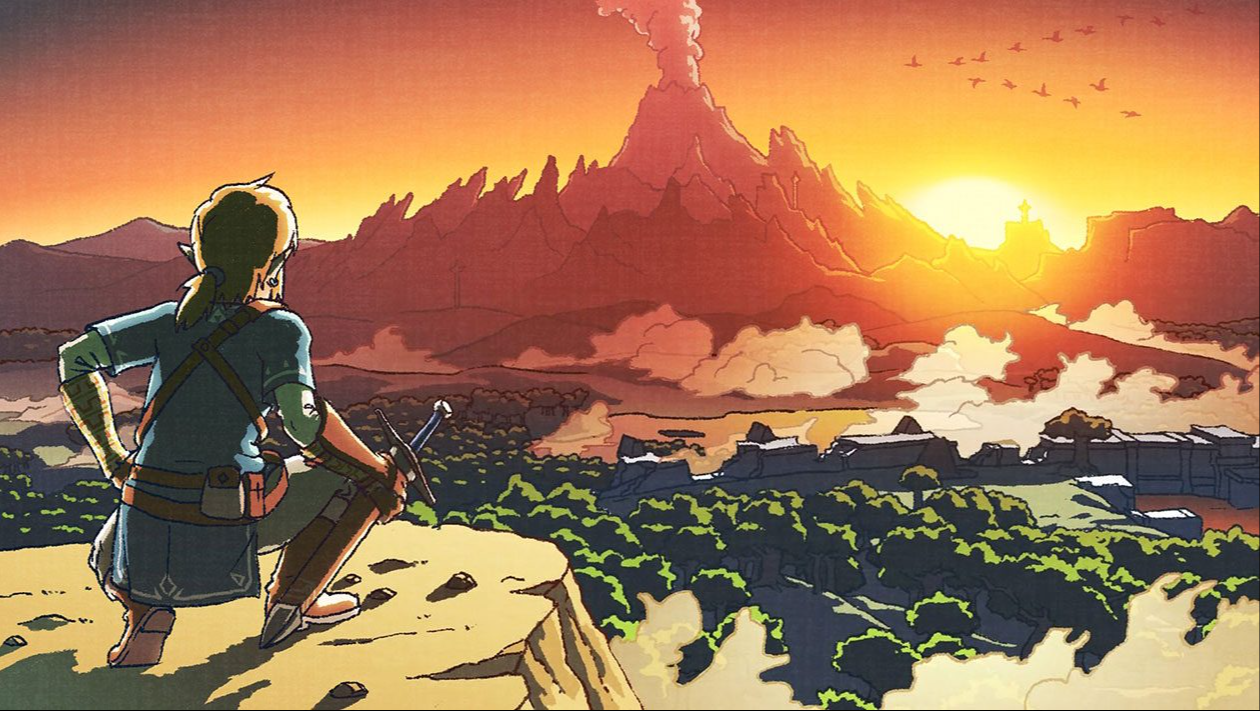
\includegraphics[width=\textwidth]{Imagenes/Referencias/conceptart_a_analizar_2.png}
        \caption{Concept art to analyze.}
    \end{figure}
    \newpage
        \subsection{Perspective}
            \subsubsection{Horizon line}
                \begin{figure}[H]
                    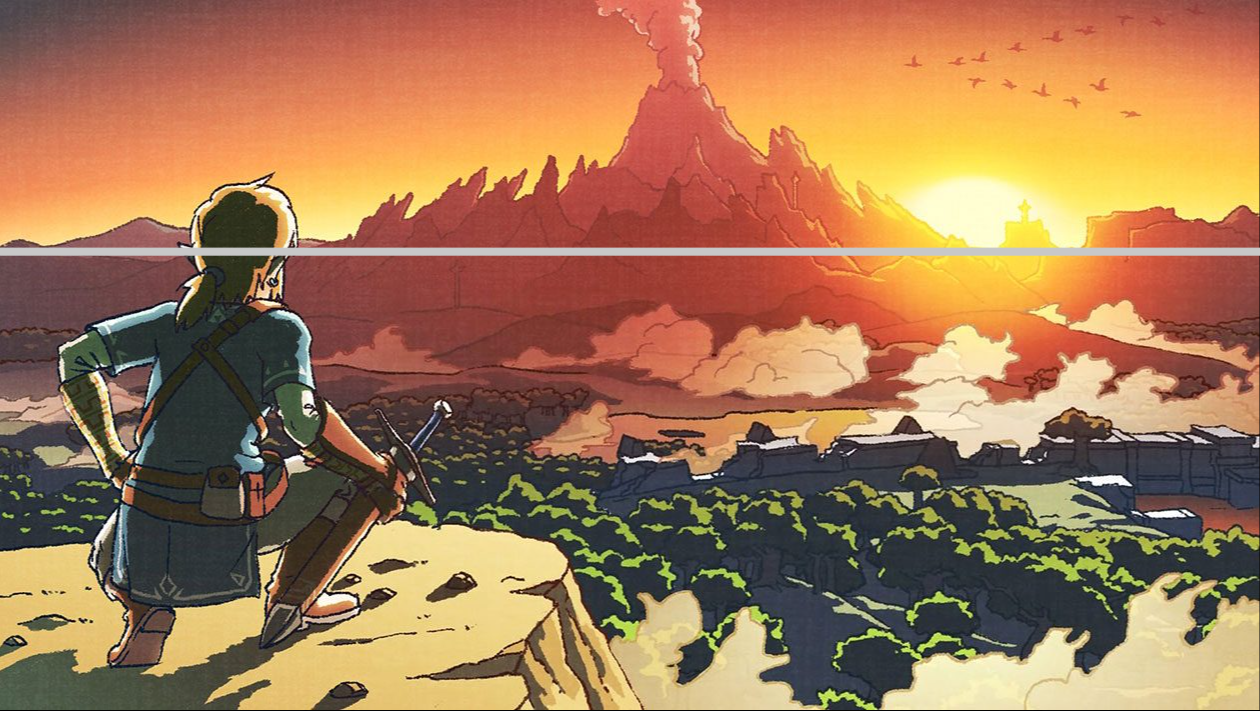
\includegraphics[width=\textwidth]{Imagenes/Referencias/Analisis_ConceptArt/horizonte.png}
                    \caption{Horizon line of the chosen concept art.}
                \end{figure}

                The horizon line is positioned a little higher from the middle, making the view point a mix of a high and low angle, but mainly a high angle. \\
            \subsubsection{Vanishing point}
                \begin{figure}[H]
                    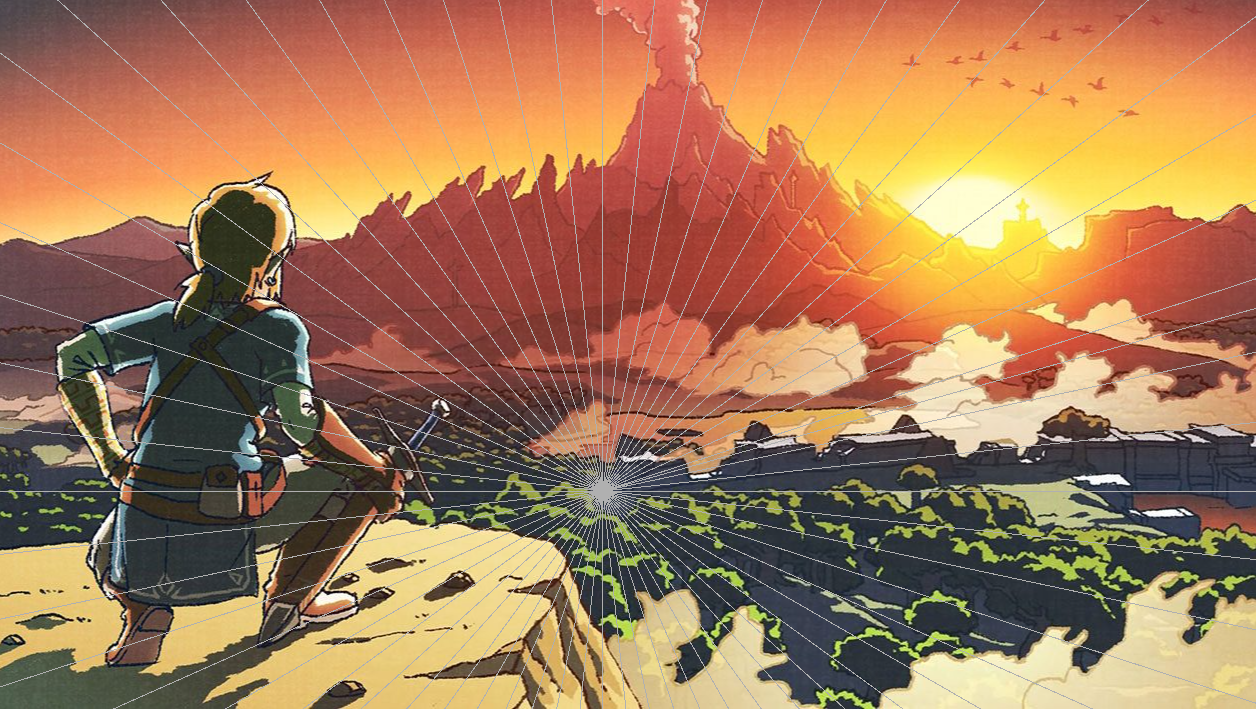
\includegraphics[width=\textwidth]{Imagenes/Referencias/Analisis_ConceptArt/posiblepuntofuga.png}
                    \caption{Possible vanishing point. (using Krita's vanishing point tool.) of the chosen concept art.}
                \end{figure}
                On this image, there's no vanishing point because of the very organic composition of the image, however, there's still a focal point that travels to the sun, which can be noticed on the rocks where Link is standing. 
                But I prefer to say that there's not a clear vanishing point because of the organic composition of the image.
        \newpage
        \subsection{Composition}
            \subsubsection{Rule of thirds}
                \begin{figure}[H]
                    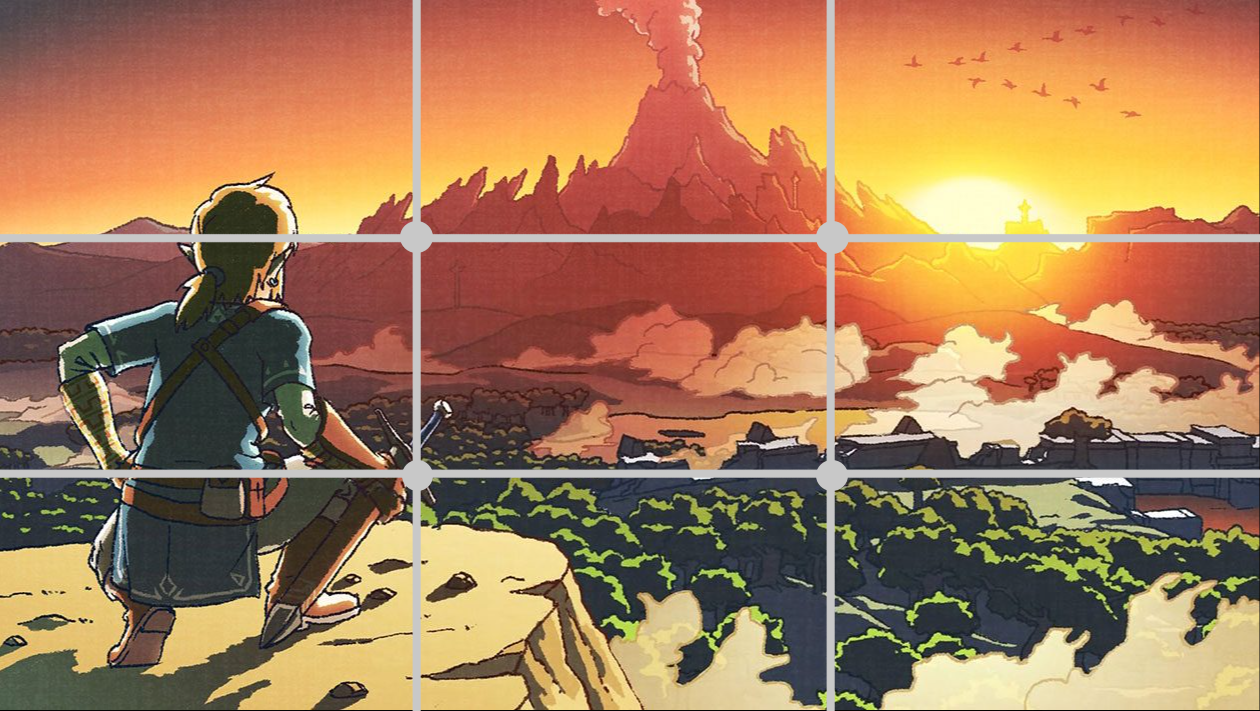
\includegraphics[width=\textwidth]{Imagenes/Referencias/Analisis_ConceptArt/tercios.png}
                    \caption{Rule of Thirds of the chosen concept art.}
                \end{figure}

                The rule of thirds is used on this image, but not in a very clear way. 
                The main subject of the image is the sun, which is placed in the top right corner of the image, but the main subject of the image is also Link at the same time.
                This creates an unbalanced composition between the two thirds.\\

            \subsubsection{Visual paths} \label{visualpaths}
                \begin{figure}[H]
                    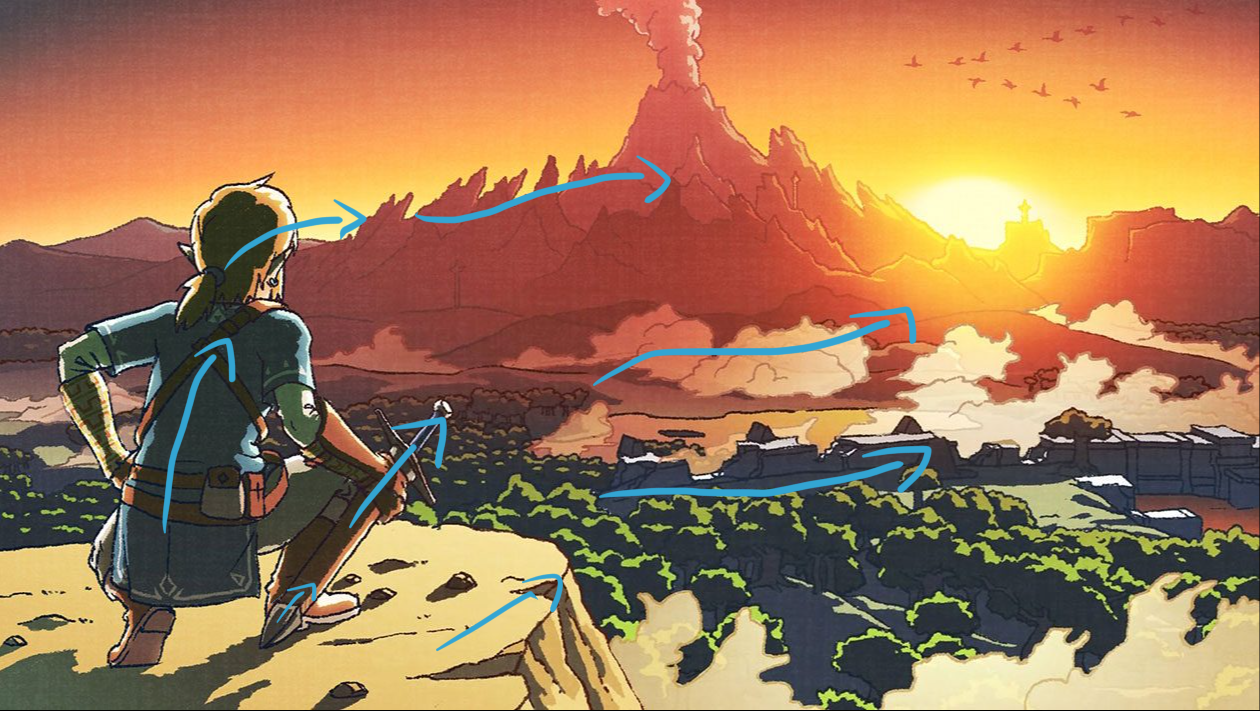
\includegraphics[width=\textwidth]{Imagenes/Referencias/Analisis_ConceptArt/recorridovisual.png}
                    \caption{Visual Paths of the chosen concept art.}
                \end{figure}

                The visual paths used on this image, flow on Link, using it's back and posture to create a visual path that goes from the bottom left corner of the image to the top right corner of the image.
                The sword is also used on the equation, taking advantage of its shape to direct the spectator view to the mountains which take the view to the corner of the composition, which where the sun is located. \\

            \subsubsection{Points of interest}
                \begin{figure}[H]
                    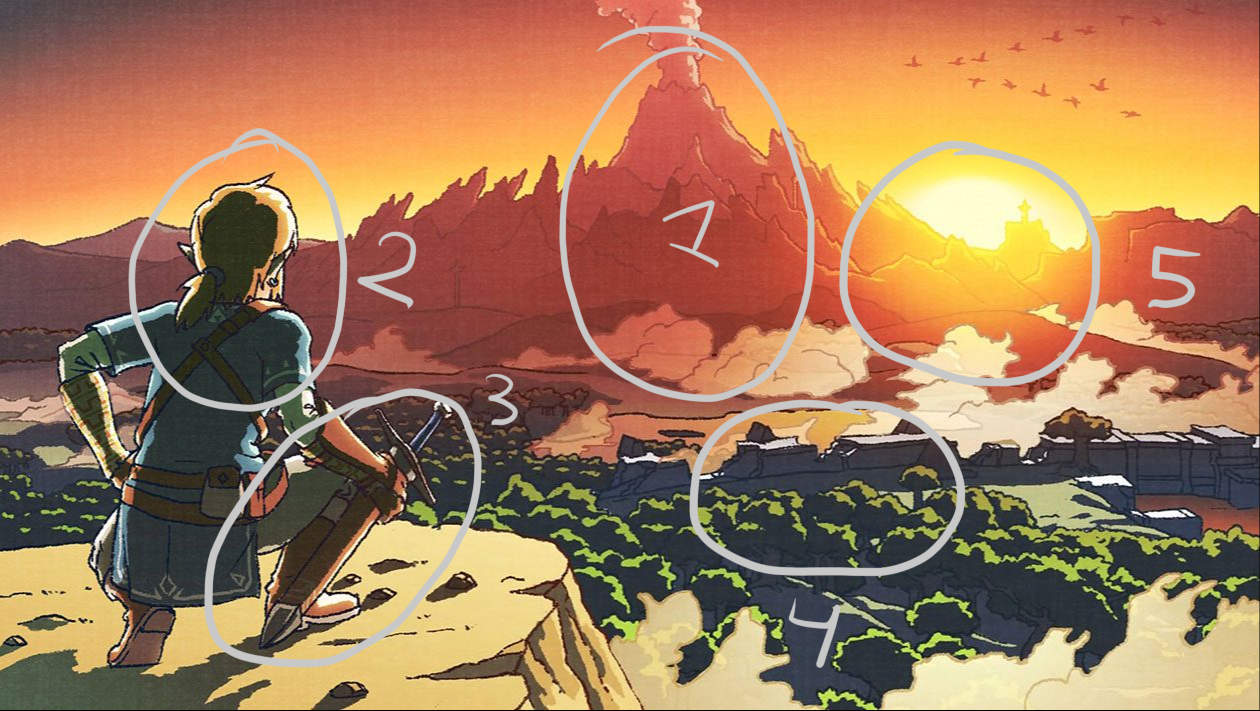
\includegraphics[width = \textwidth]{Imagenes/Referencias/Analisis_ConceptArt/puntos interes.png}
                    \caption{Points of interest of the chosen concept art.}
                \end{figure}
                There's a clear path that images provides when it needs to be read, which it's made clear when you look at the~\ref{visualpaths} section.\\

                The image starts at the mountain being at the center at the image, and because of the bright colors used on Link, the focal points shifts to Link and his sword, which takes you to the small forest / destroyed wall, and then ending in the sun.\\

            \subsubsection{Balance}
                \begin{figure}[H]
                    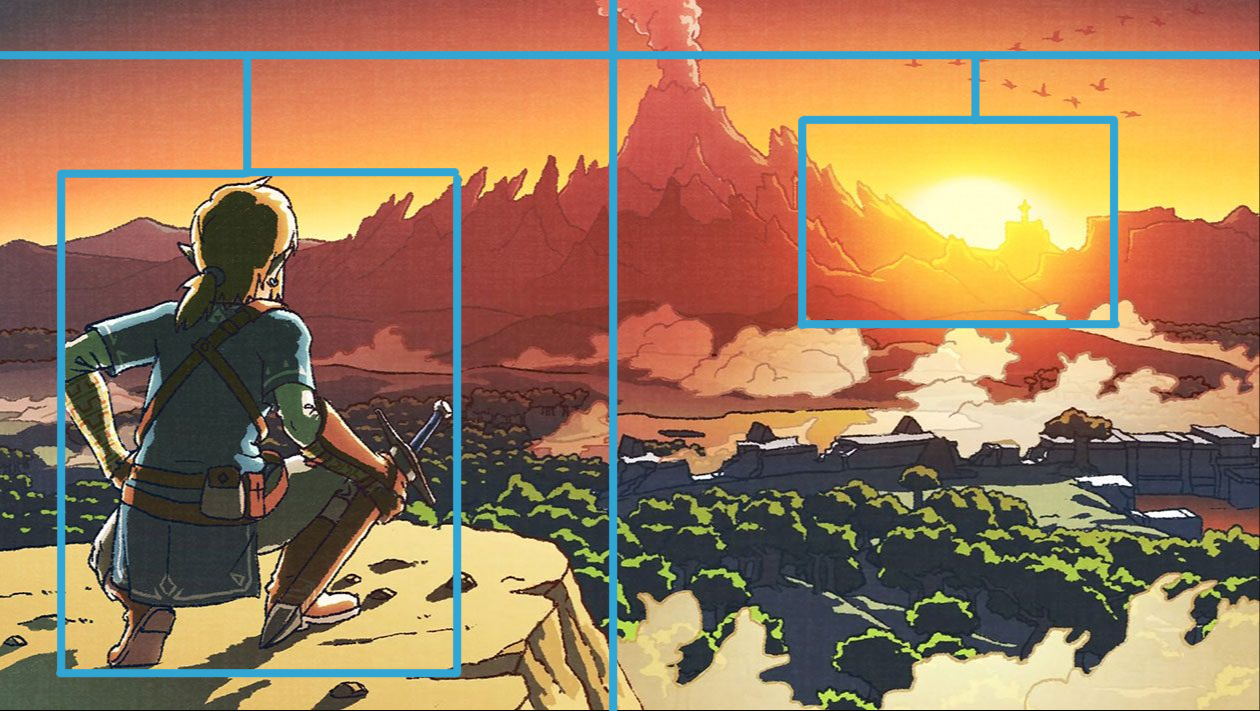
\includegraphics[width=\textwidth]{Imagenes/Referencias/Analisis_ConceptArt/balanza.png}
                    \caption{Weight Balance of the chosen concept art.}
                \end{figure}
                The image can be considered unbalanced on both sides, on the right side you have the sun, which is very bright and has a lot of contrast, but on the left side you have Link which his silhouette makes it stand up from the rest of the composition. 
        \newpage
        \subsection{Chiaroscuro}
            \begin{figure}[H]
                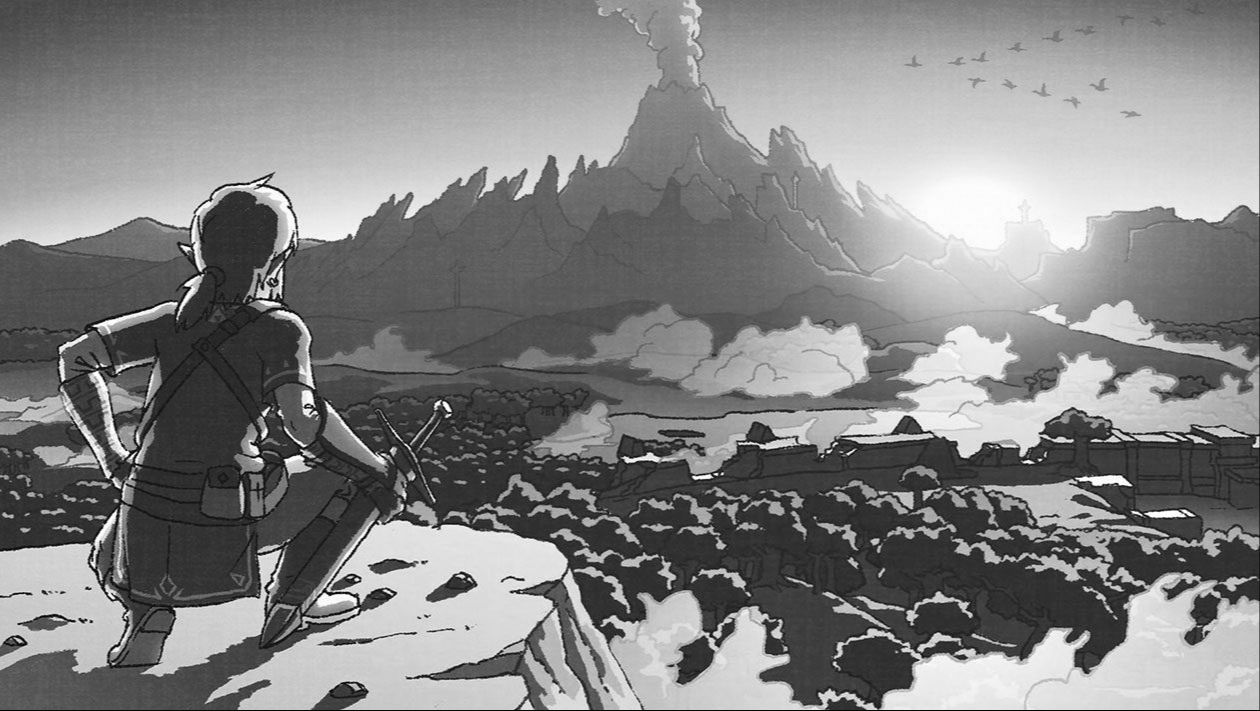
\includegraphics[width=\textwidth]{Imagenes/Referencias/Analisis_ConceptArt/claroscuro.png}
                \caption{Chiaroscuro of the chosen concept art.}
            \end{figure}

            The chiaroscuro on this image makes even more clear what the focus of the image is middle key, because of the sun being very bright compared to the mountains which contribute to the image being middle key which is also reinforced by the shadow covering Link.\\
            \begin{figure}[H]
                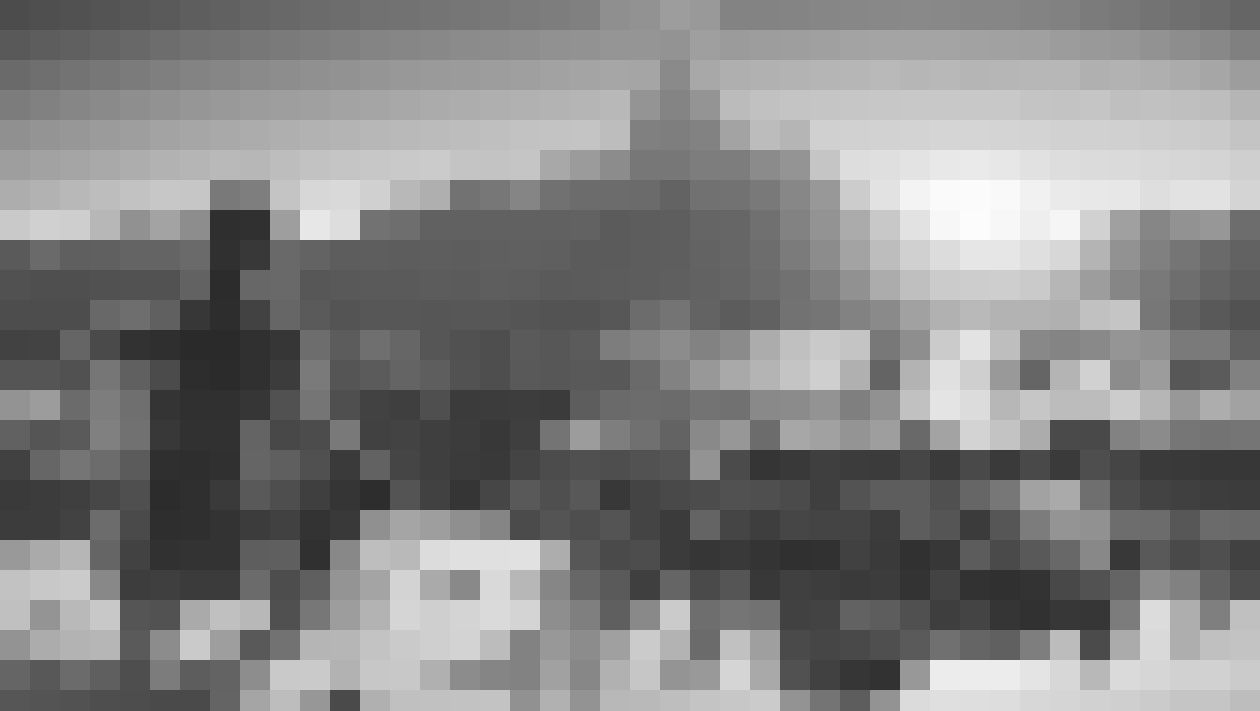
\includegraphics[width=\textwidth]{Imagenes/Referencias/Analisis_ConceptArt/pixel.png}
                \caption{Pixelizated Chiaroscuro of the chosen concept art.}
            \end{figure}

            If we pixelate the chiaroscuro, the image reveals main source of the light, which is drawn below the pixelization. 
            \begin{figure}[H]
                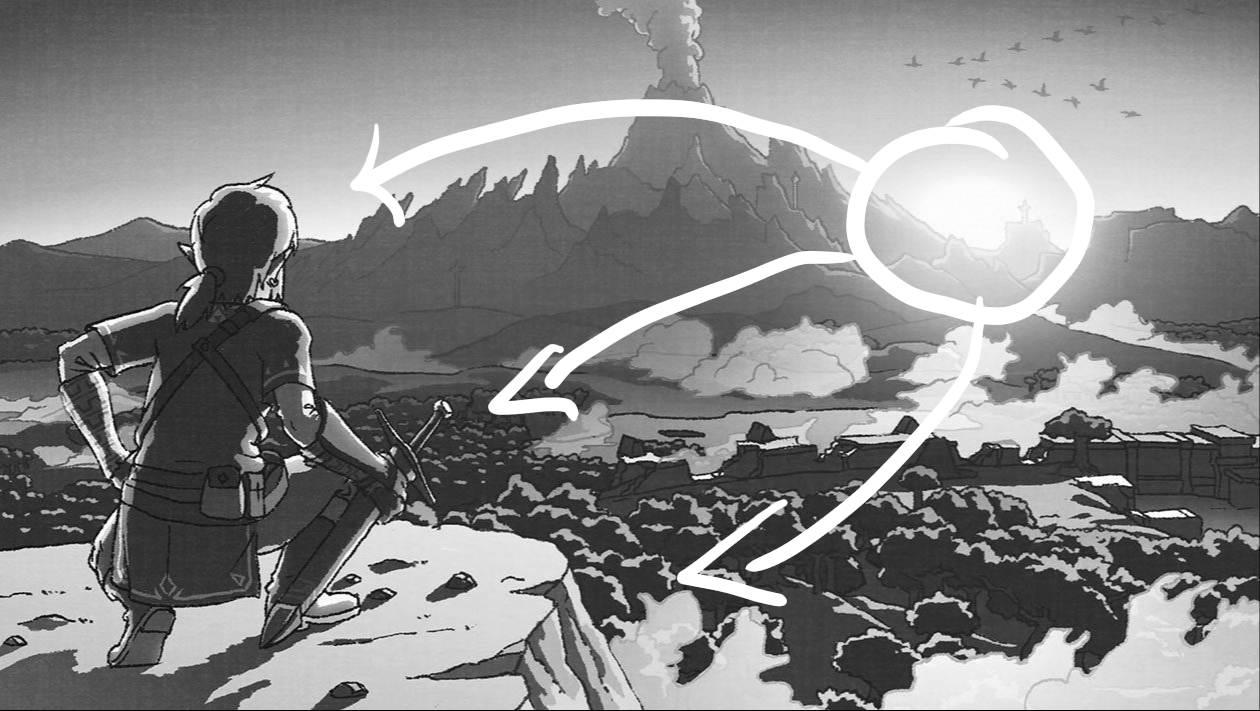
\includegraphics[width=\textwidth]{Imagenes/Referencias/Analisis_ConceptArt/recorrido luz.png}
                \caption{Light Path of the chosen concept art.}
            \end{figure}

            Continuing from the previous point, we can see that the light is coming from the top right corner of the image, which is the sun and bleeds through the image making the contrast between Link and the scenery.\\
        \newpage
        \subsection{Color}

            The color is one of the reasons of why this image is so appealing, the color palette is very warm, and the tonality is very bright, which makes the image very appealing.\\
             \begin{figure}[H]
                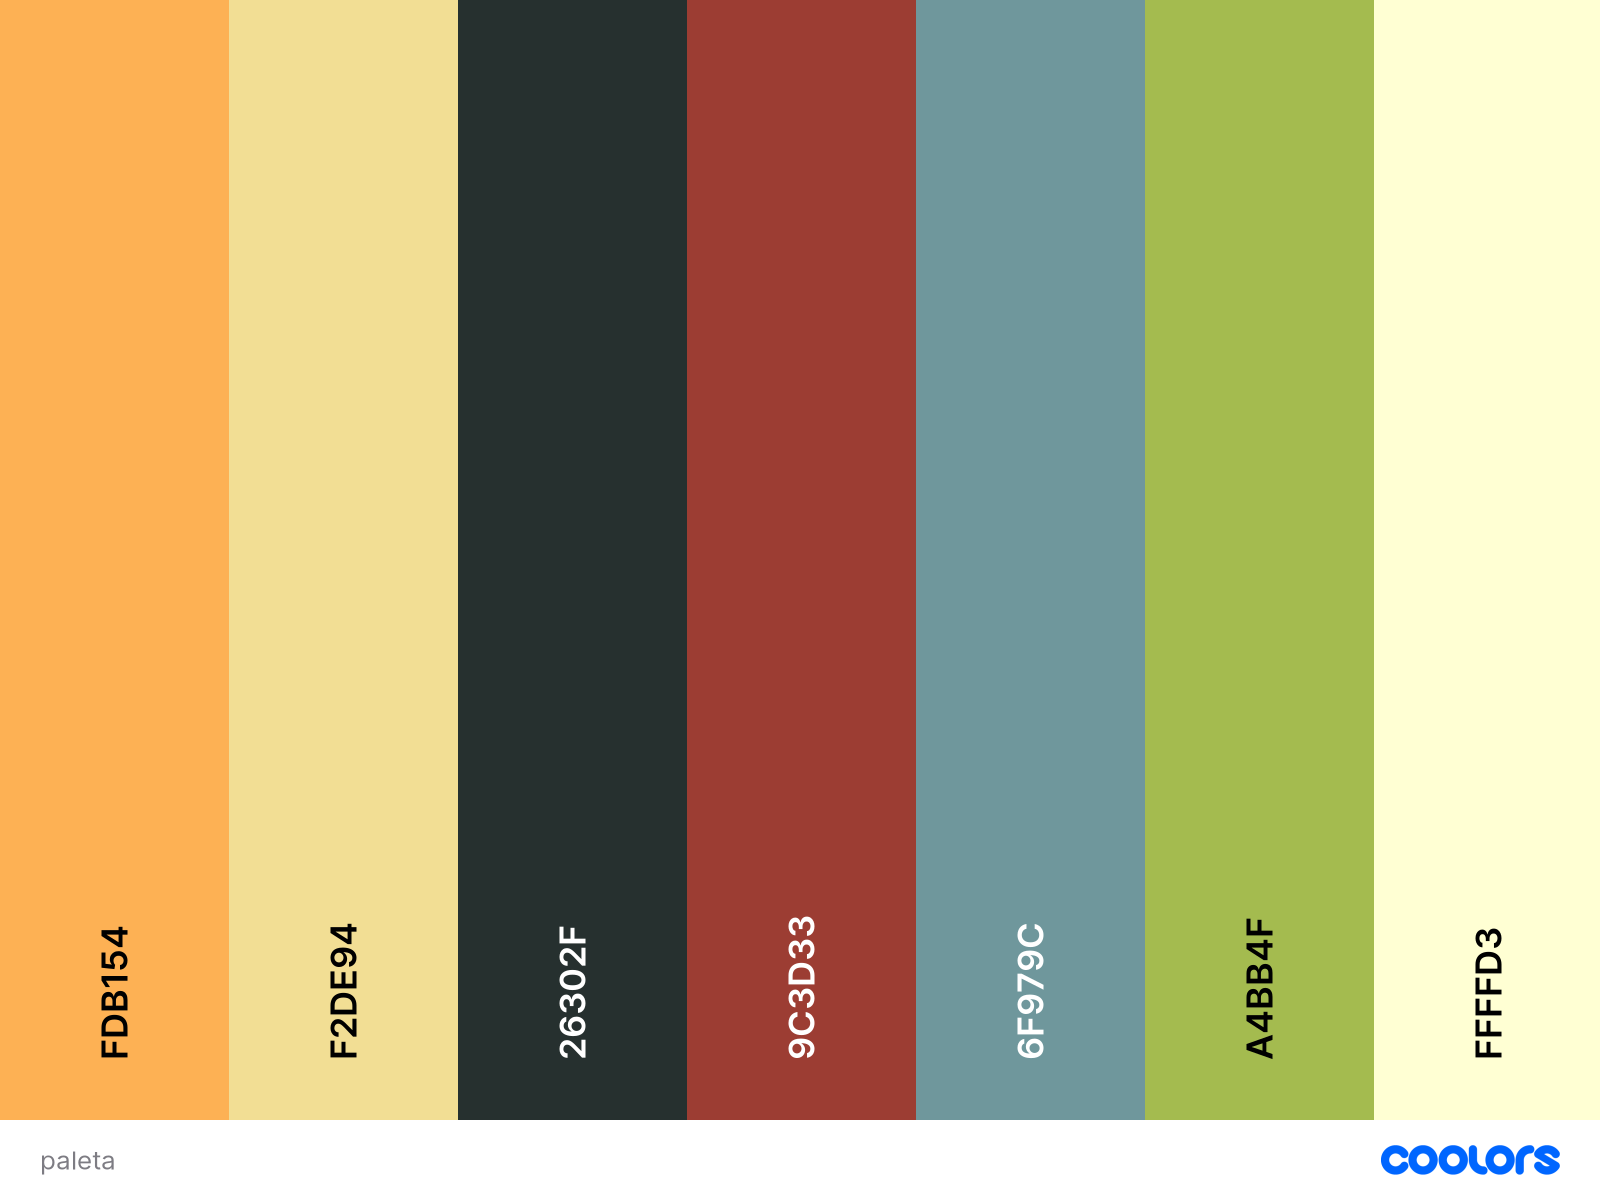
\includegraphics[width=\textwidth]{Imagenes/Referencias/Analisis_ConceptArt/paleta.png}
                \caption{Color Palette of the chosen concept art.}
            \end{figure}

            As I previously mentioned, the color palette is very warm, using bright yellowy and reds and making tonality contrast with the blue on Link's shirt.
            The greens used in the forest which also resonate with the gray used on the destroyed wall. \\
            \begin{figure}[H]
                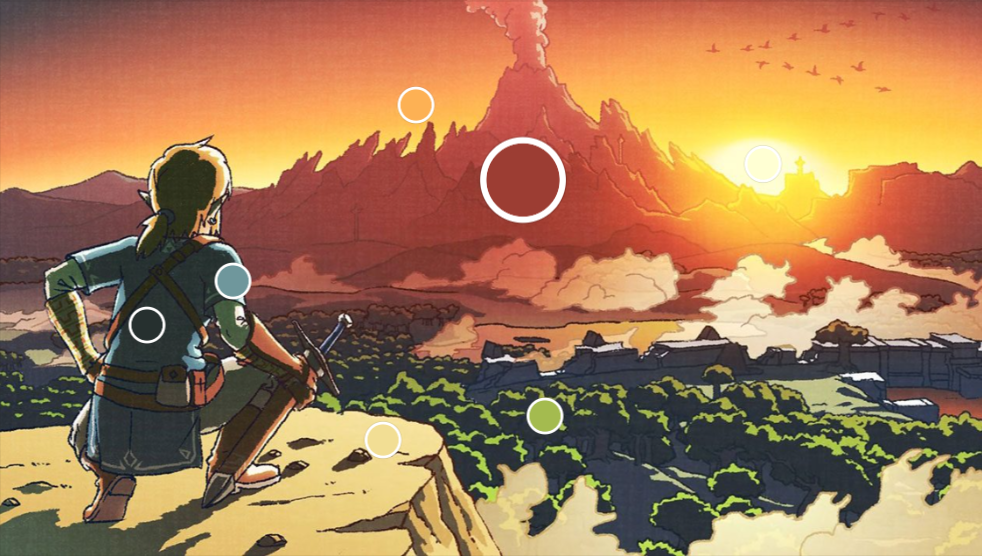
\includegraphics[width=\textwidth]{Imagenes/Referencias/Analisis_ConceptArt/tonalidad.png}
                \caption{Color Tonality of the chosen concept art.}
            \end{figure}

            The image, is broad terms, screams \textit{contrast}. Some examples of how contrast is used:
            \begin{itemize}
                \item Saturation contrast: Used to differentiate the colors used on the mountains and separate far away mountains from closer ones.
                \item Luminance contrast: Used on Link's shirt to make the shadows. 
                \item Tonal contrast: Used on the sun (yellow) and the forest (green). 
            \end{itemize}
            \begin{figure}[H]
                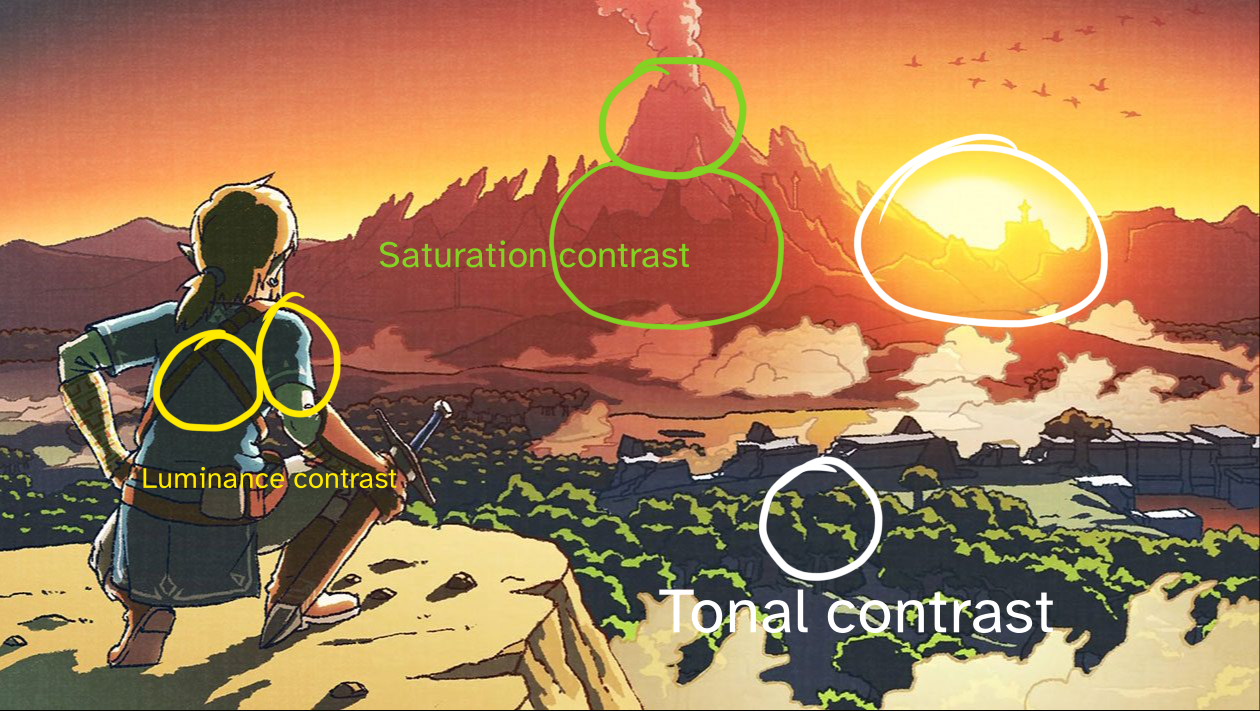
\includegraphics[width=\textwidth]{Imagenes/Referencias/Analisis_ConceptArt/contrast.png}
                \caption{Color Contrast of the chosen concept art.}
            \end{figure}

%%______________________________________________________________________________
%%______________________________________________________________________________

\newpage
\section{First Illustration}
    \subsection{Line art and sketches}

        The first fan art was the most difficult to make, because it was the first time I made a fan art and I didn't know how to start. So I started with a simple sketch of the Dueling Peaks. 
        I also used the Blocks Rig previously mentioned to quickly pose a character.\\
        \begin{figure}[H]
            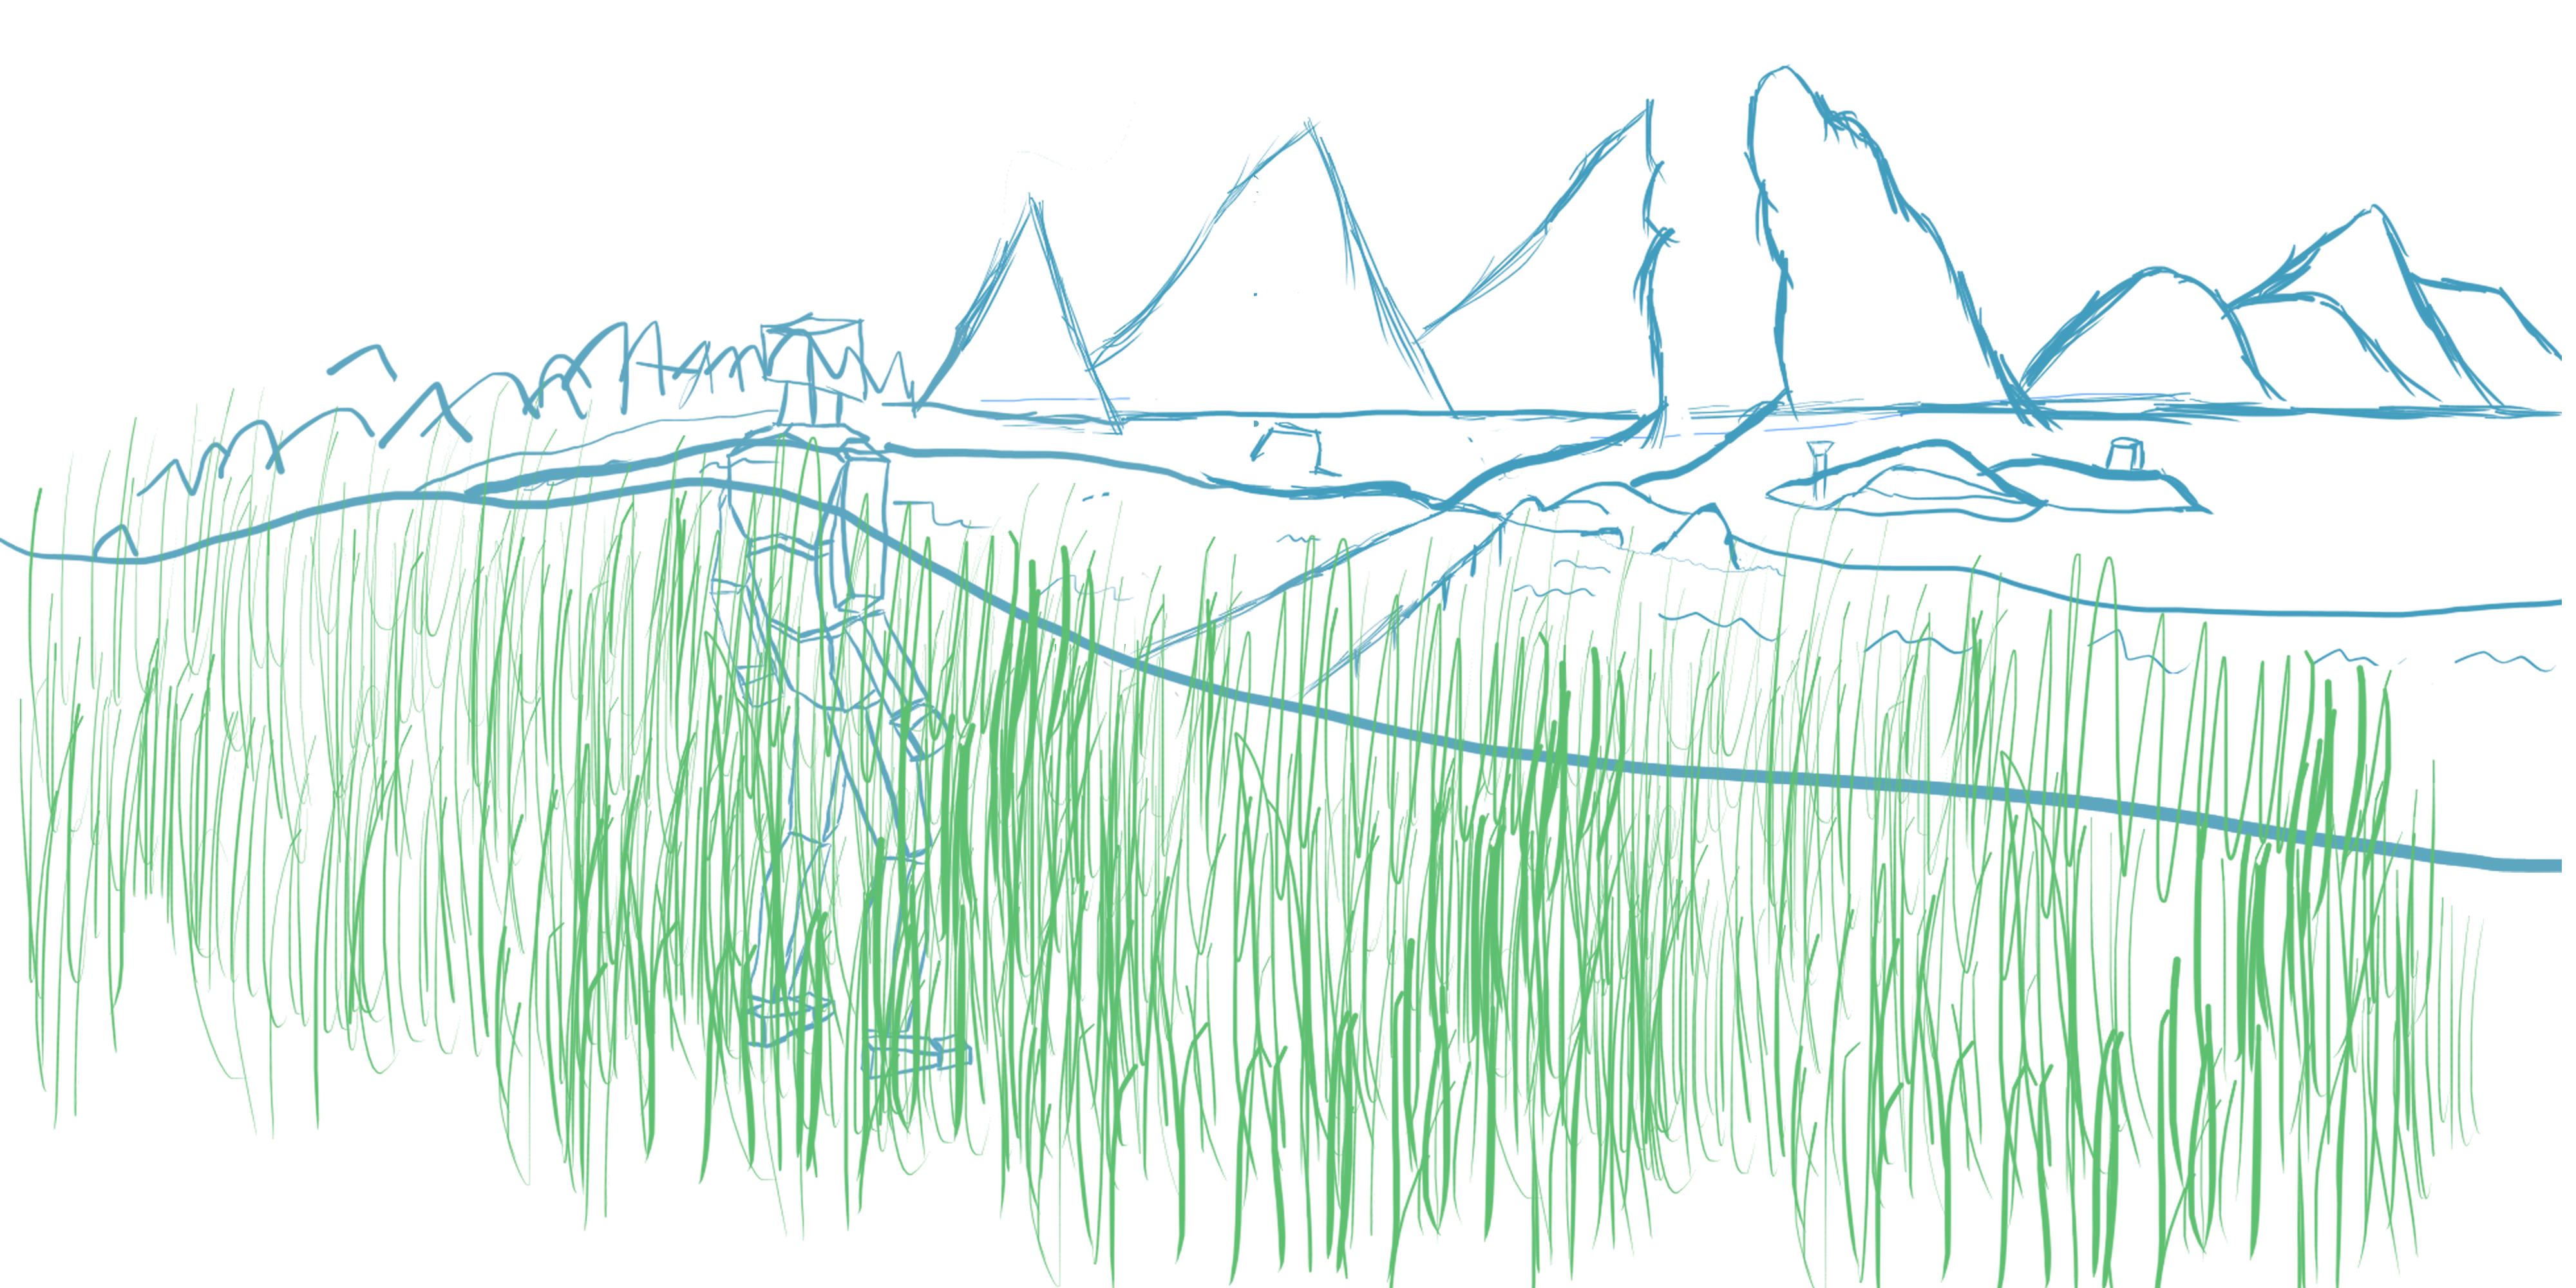
\includegraphics[width=\textwidth]{Imagenes/Fanart1/Boceto_Lineart/0 Imagen de partida.png}
            \caption{First sketch of the Dueling Peaks.}
        \end{figure}

        On the first iteration, I used the previous art on the “Composition I” assignment, by using images from the game and reality to make a quick sketch of how the art would look like.\\
        \begin{figure}[H]
            \includegraphics[width=\textwidth]{Imagenes/Fanart1/Boceto_Lineart/1a_Iteracion.jpg}
            \caption{First iteration of the Dueling Peaks, using images as reference.}
        \end{figure}

        On the second iteration, I improved upon the reference images and added more details and tried to make everything consistent in the drawing.\\
        \begin{figure}[H]
            \includegraphics[width=\textwidth]{Imagenes/Fanart1/Boceto_Lineart/2a_iteración.png}
            \caption{Second iteration of the Dueling Peaks.}
        \end{figure}

        On the third iteration, I polished the strokes and added more details to the sketch. Also, I added the grass and some clouds, filling them with a \textit{watery} brush to give it a more \textit{cloudy} feeling.\\
        \begin{figure}[H]
            \includegraphics[width=\textwidth]{Imagenes/Fanart1/Boceto_Lineart/3a_iteracion.png}
            \caption{Third iteration of the Dueling Peaks.}
        \end{figure}

        To end with this step, I cleaned up the clouds and removed the coloring. I also changed the blocks rig character for a new one, which was the Zelda Rig.\\
        \begin{figure}[H]
            \includegraphics[width=\textwidth]{Imagenes/Fanart1/Boceto_Lineart/4a_Iteracion.png}
            \caption{Fourth iteration of the Dueling Peaks.}
        \end{figure}

    \subsection{Chiaroscuro}
        Commencing with the chiaroscuro, I sketched how would the blacks and whites would progress naturally to the end of the composition.
        \begin{figure}[H]
            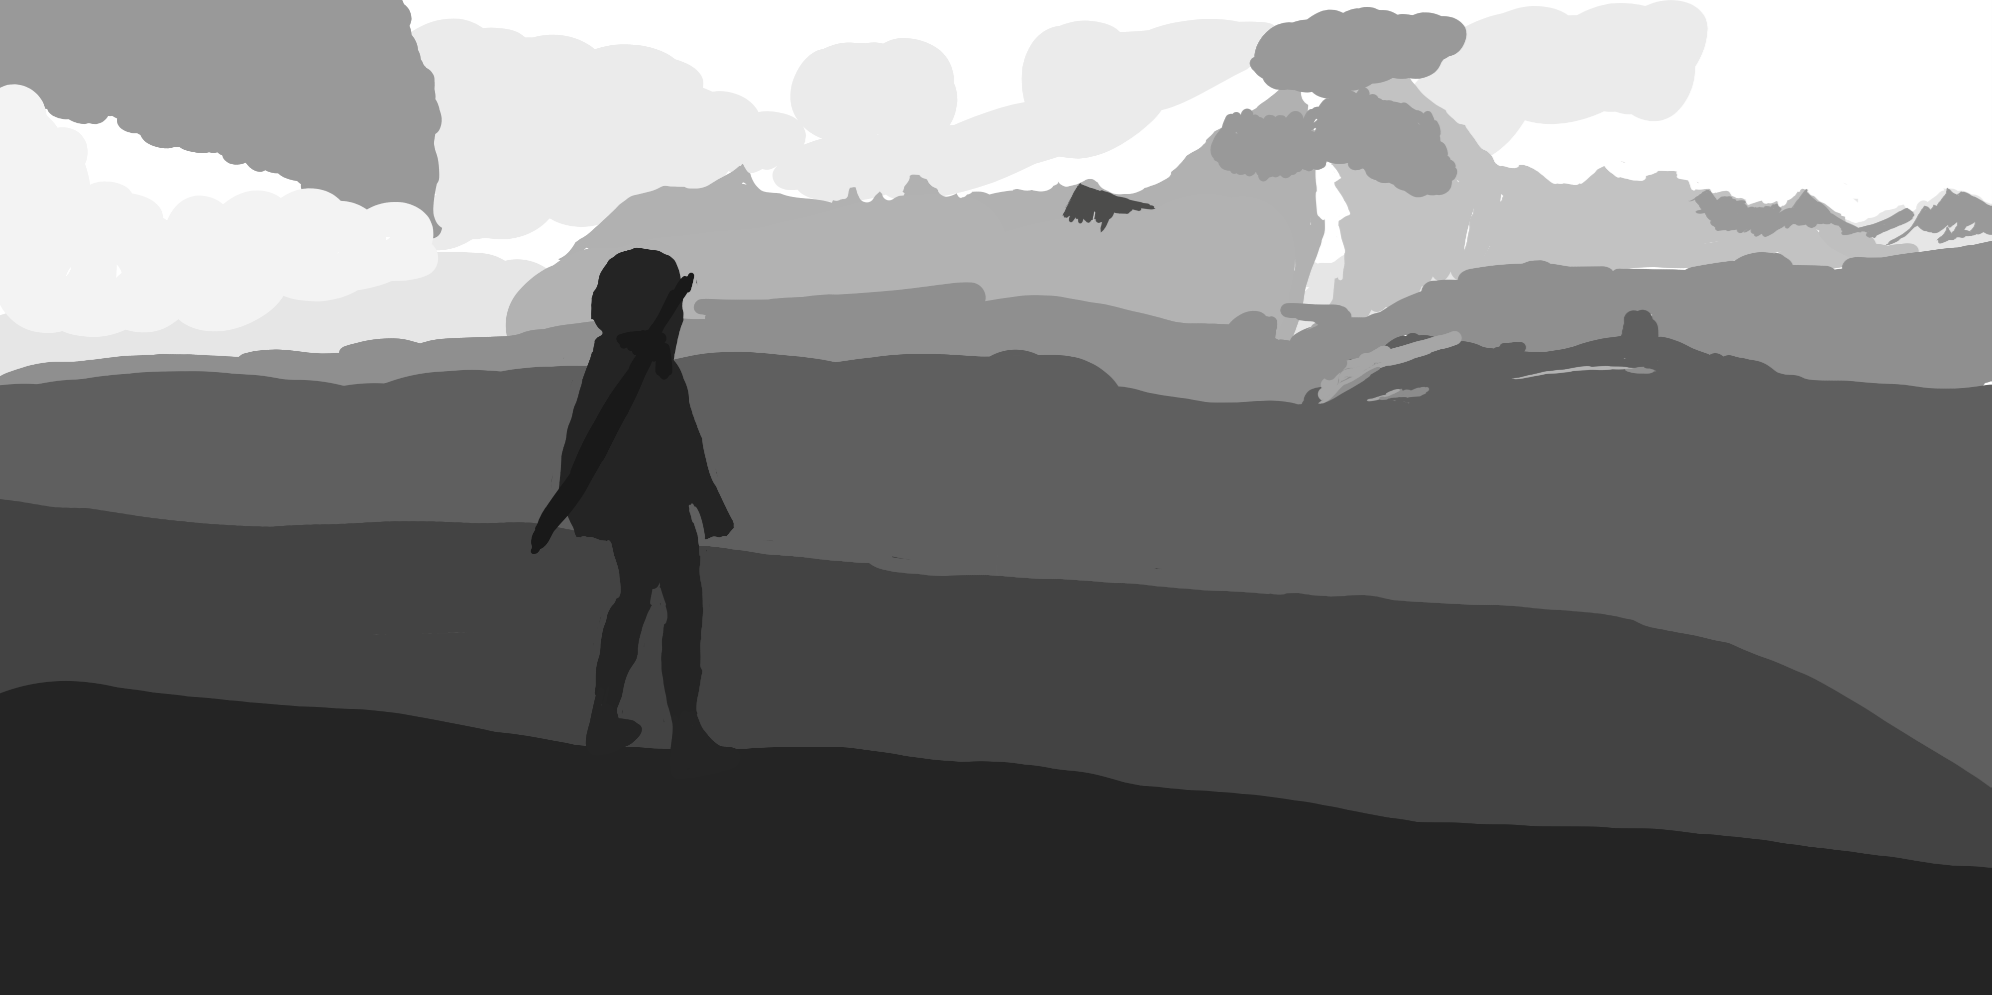
\includegraphics[width=\textwidth]{Imagenes/Fanart1/Claroscuro/Imagen1.png}
            \caption{First iteration of the chiaroscuro.}
        \end{figure}

        On the second iteration, I added more details to the chiaroscuro, making it more consistent with the line art, but the character was done at a later iteration to keep the focus on the scenery.\\
        \begin{figure}[H]
            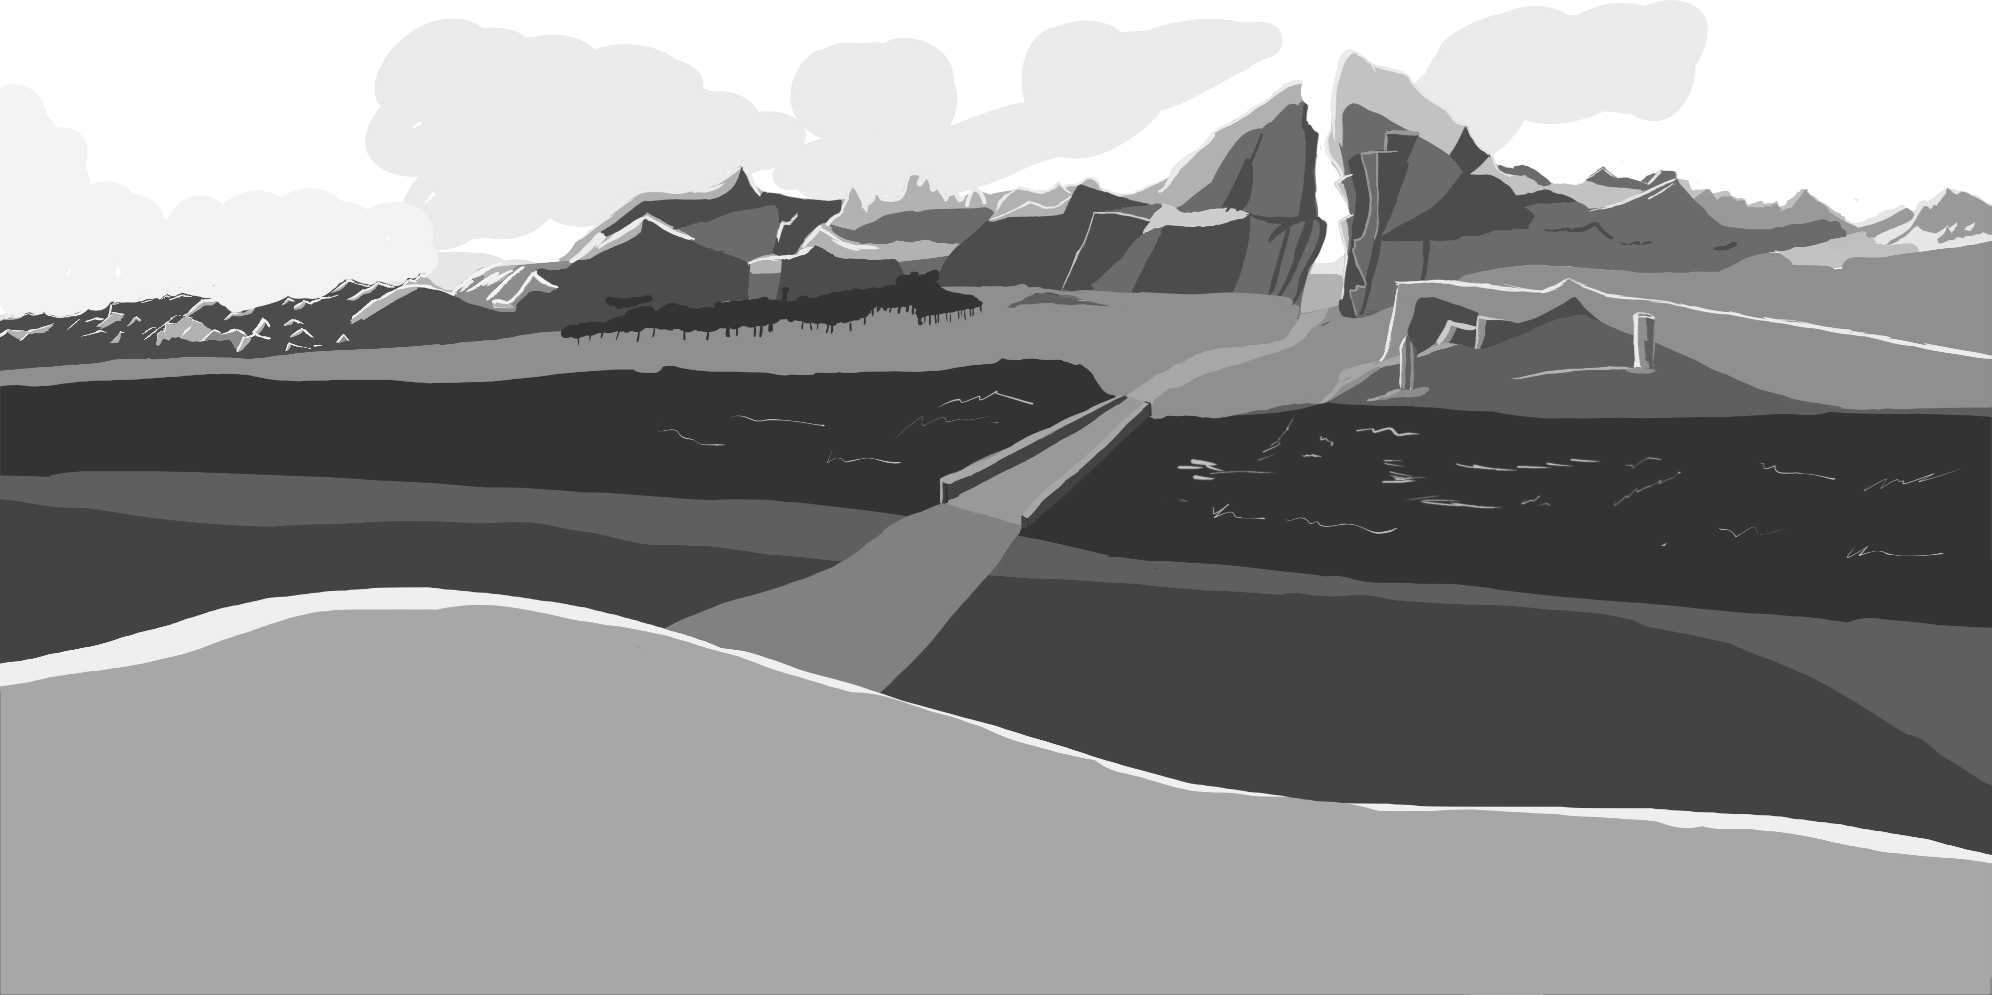
\includegraphics[width=\textwidth]{Imagenes/Fanart1/Claroscuro/Imagen2.png}
            \caption{Second iteration of the chiaroscuro.}
        \end{figure}

        On the third iteration, I added more details to the chiaroscuro, with some rudimentary shadows and a basic shading, with more clouds added and a basic silhouette of the character.\\
        \begin{figure}[H]
            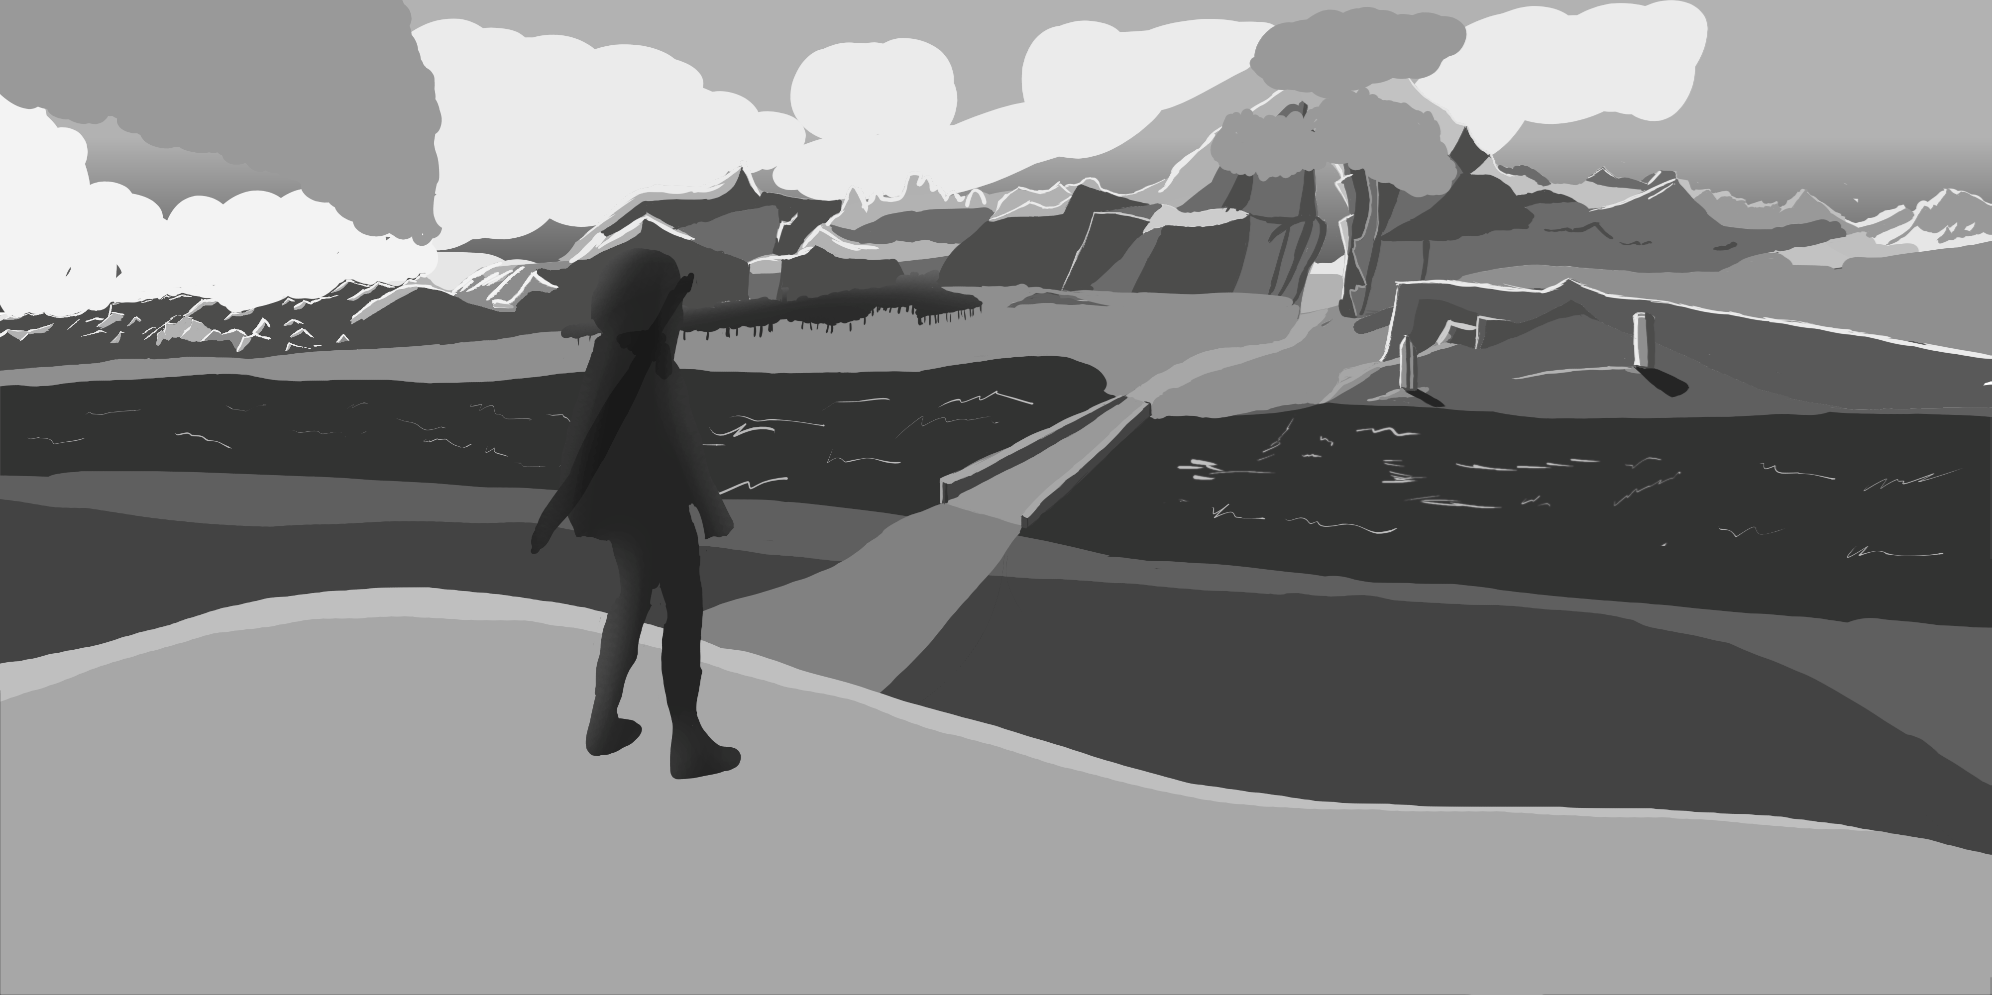
\includegraphics[width=\textwidth]{Imagenes/Fanart1/Claroscuro/Imagen3.png}
            \caption{Third iteration of the chiaroscuro.}
        \end{figure}

        On the fourth iteration, I added detail to the character and a shadow to it. Also, I added shading to the mountains, character, river, and the bridge. This was made to separate everything much better than using just a simple black and white scheme.\\
        \begin{figure}[H]
            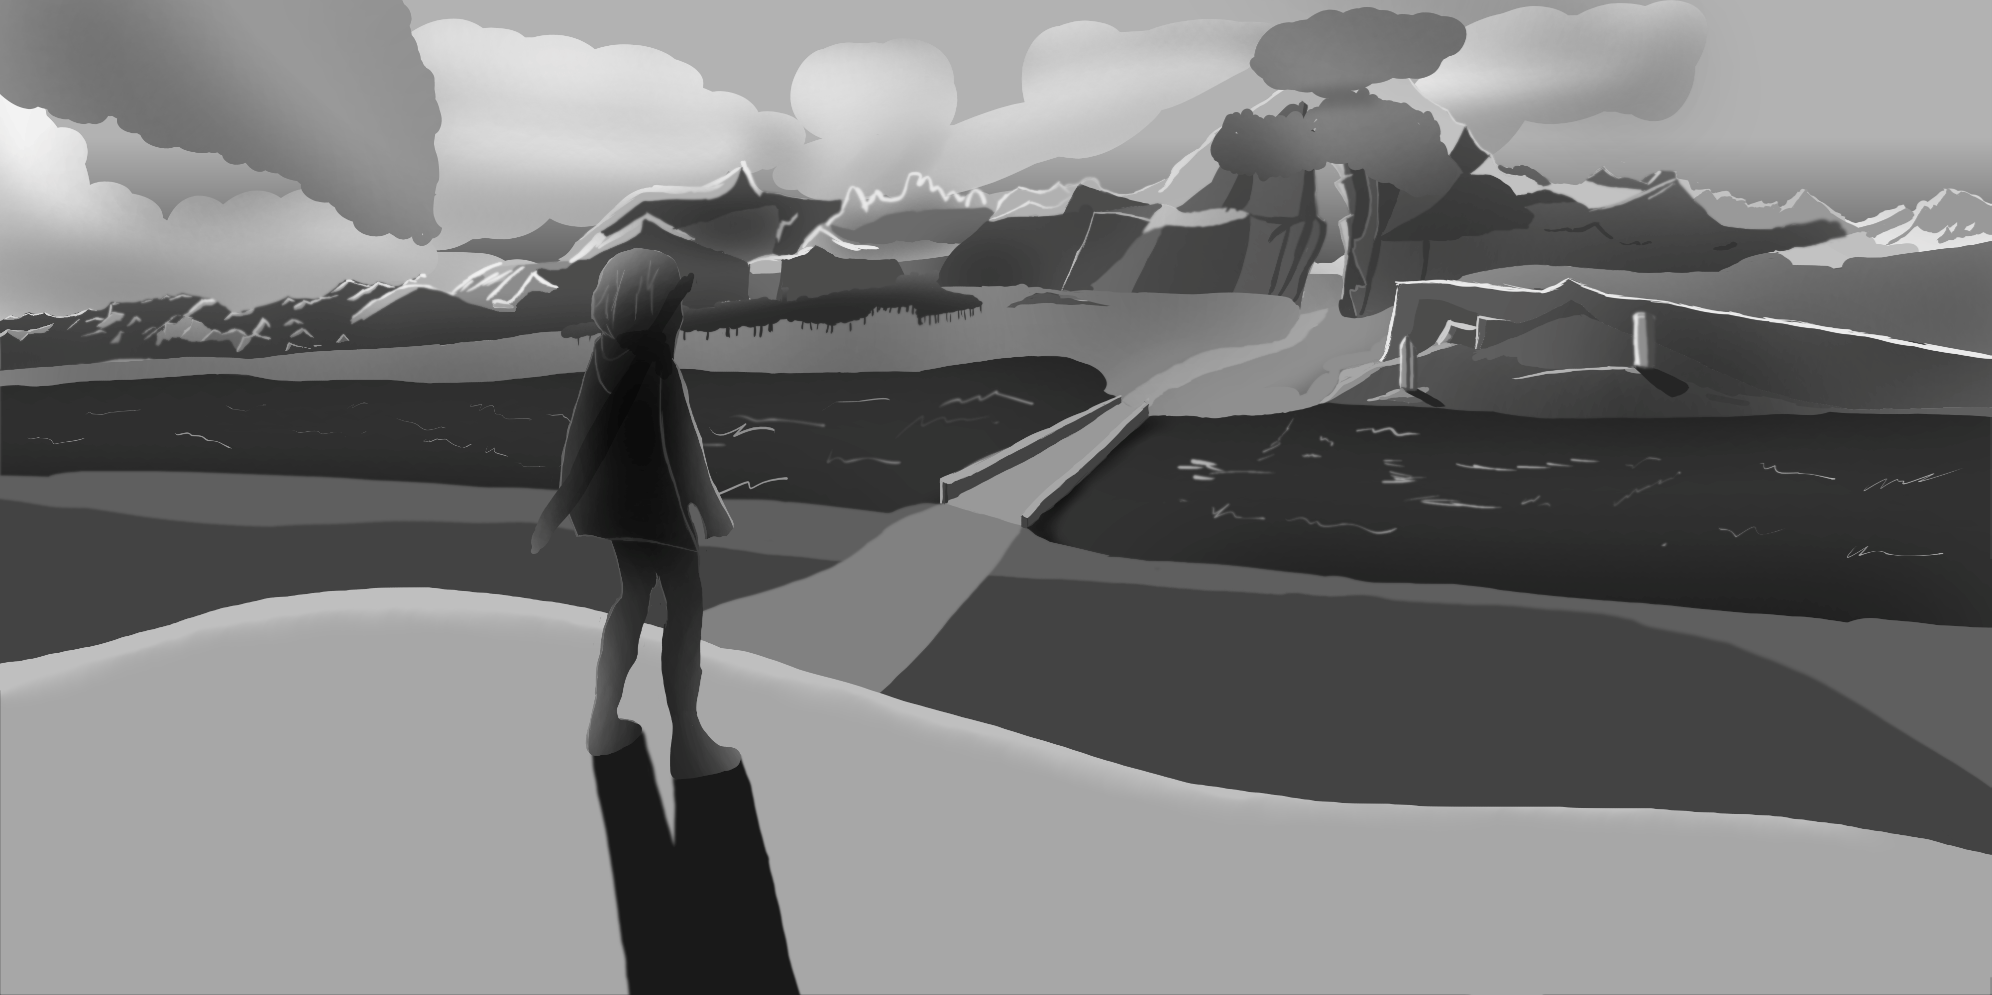
\includegraphics[width=\textwidth]{Imagenes/Fanart1/Claroscuro/Imagen4.png}
            \caption{Fourth iteration of the chiaroscuro.}
        \end{figure}

    \subsection{Coloring}
        The coloring part of this fan arts had fewer parts overall, because the chiaroscuro was already done and techniques taught in class were used. Basically, adding a “Color” layer and applying the color from there.\\

        On the first iteration, I added the colors to the chiaroscuro, making the mountains a bit more saturated and adding a bit of color  to the sky and the small forest in the distance.\\
        \begin{figure}[H]
            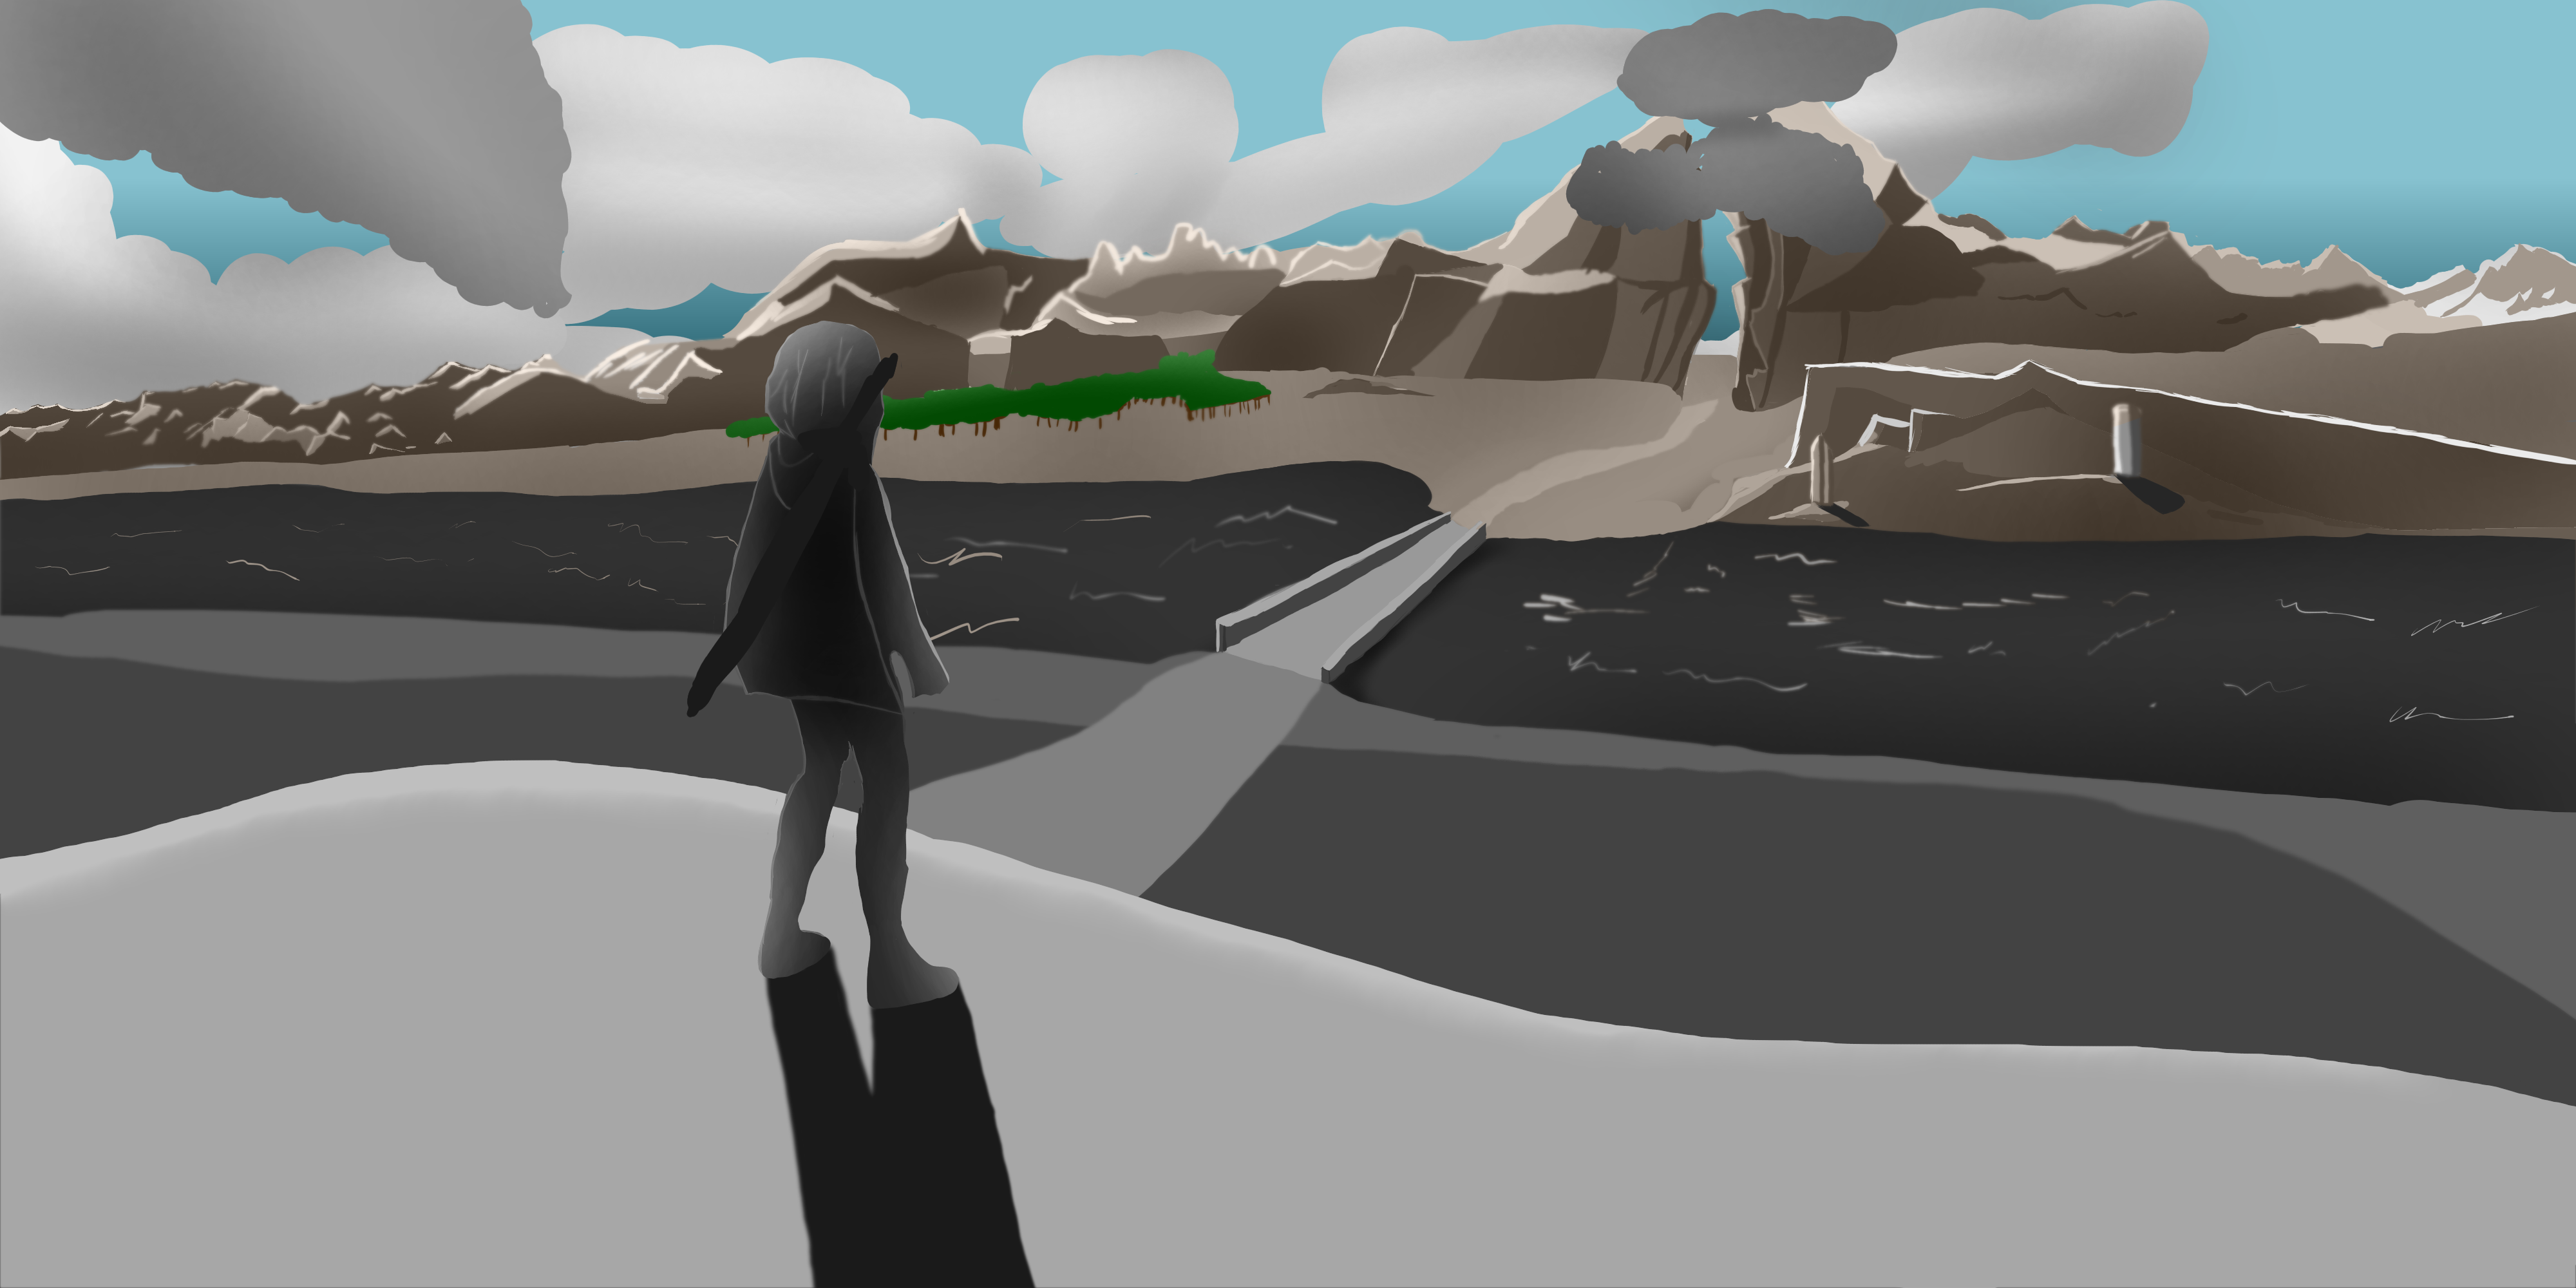
\includegraphics[width=\textwidth]{Imagenes/Fanart1/Color/I_Iteracion.png}
            \caption{First iteration of the coloring.}
        \end{figure}
        
        On the second iteration, I added colors to the river and the hill. 
        \begin{figure}[H]
            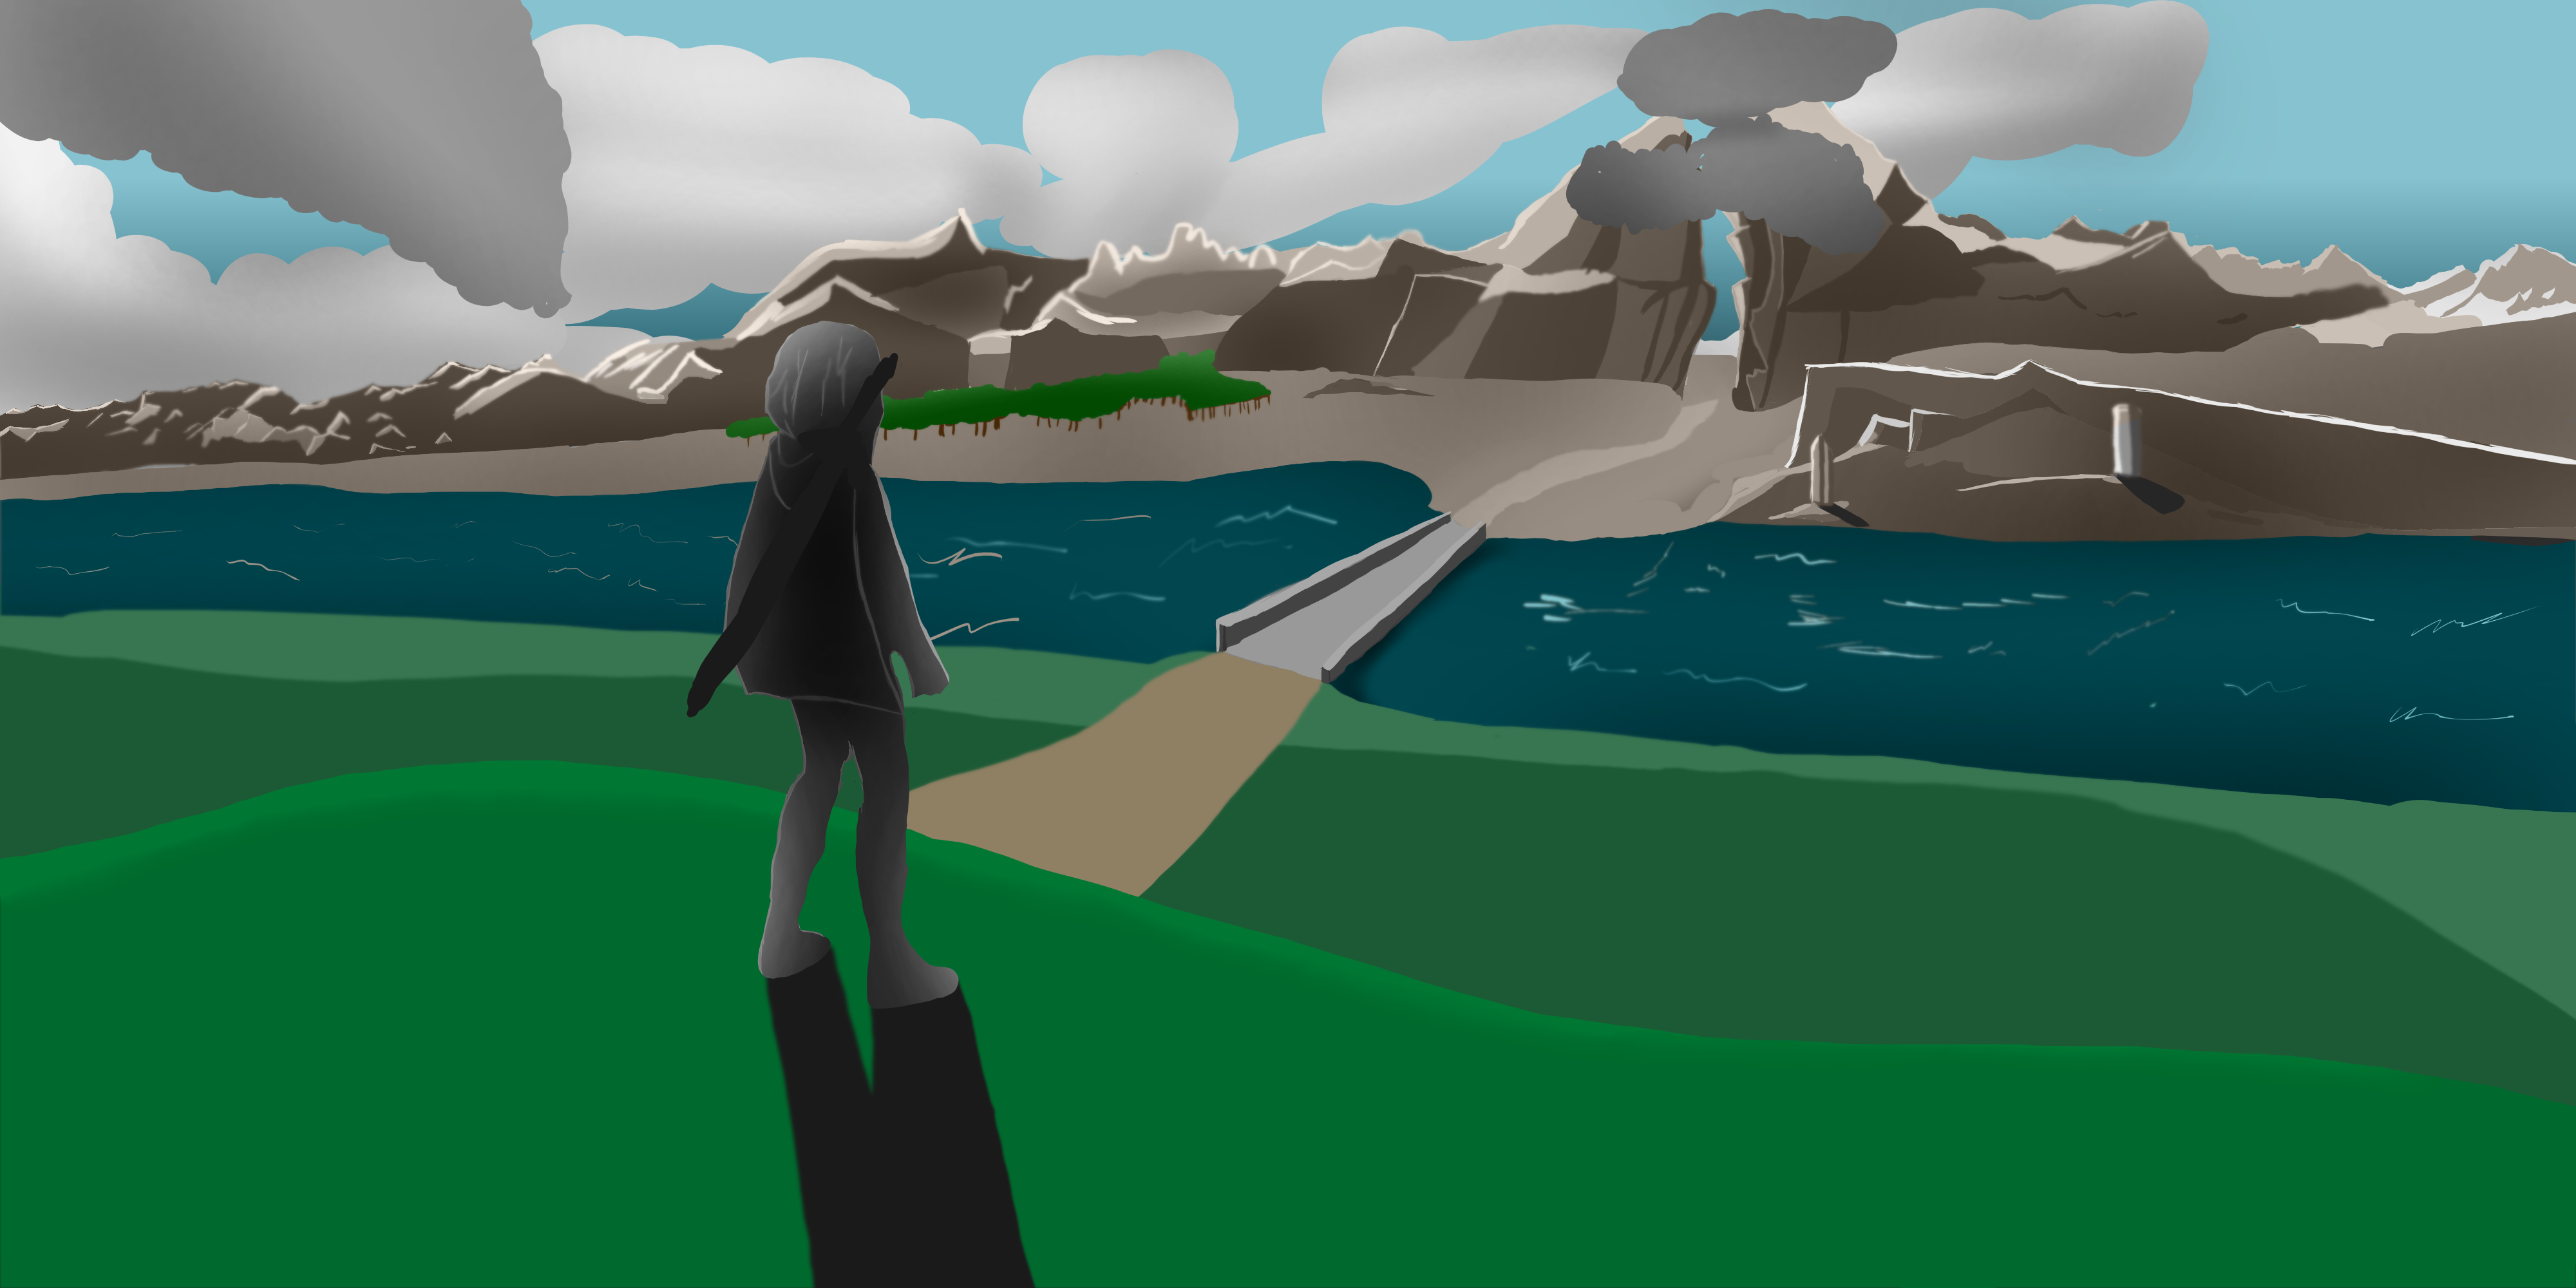
\includegraphics[width=\textwidth]{Imagenes/Fanart1/Color/II_Iteracion.png}
            \caption{Second iteration of the coloring.}
        \end{figure}

        On the third iteration I added some colors to Zelda. 
        \begin{figure}[H]
            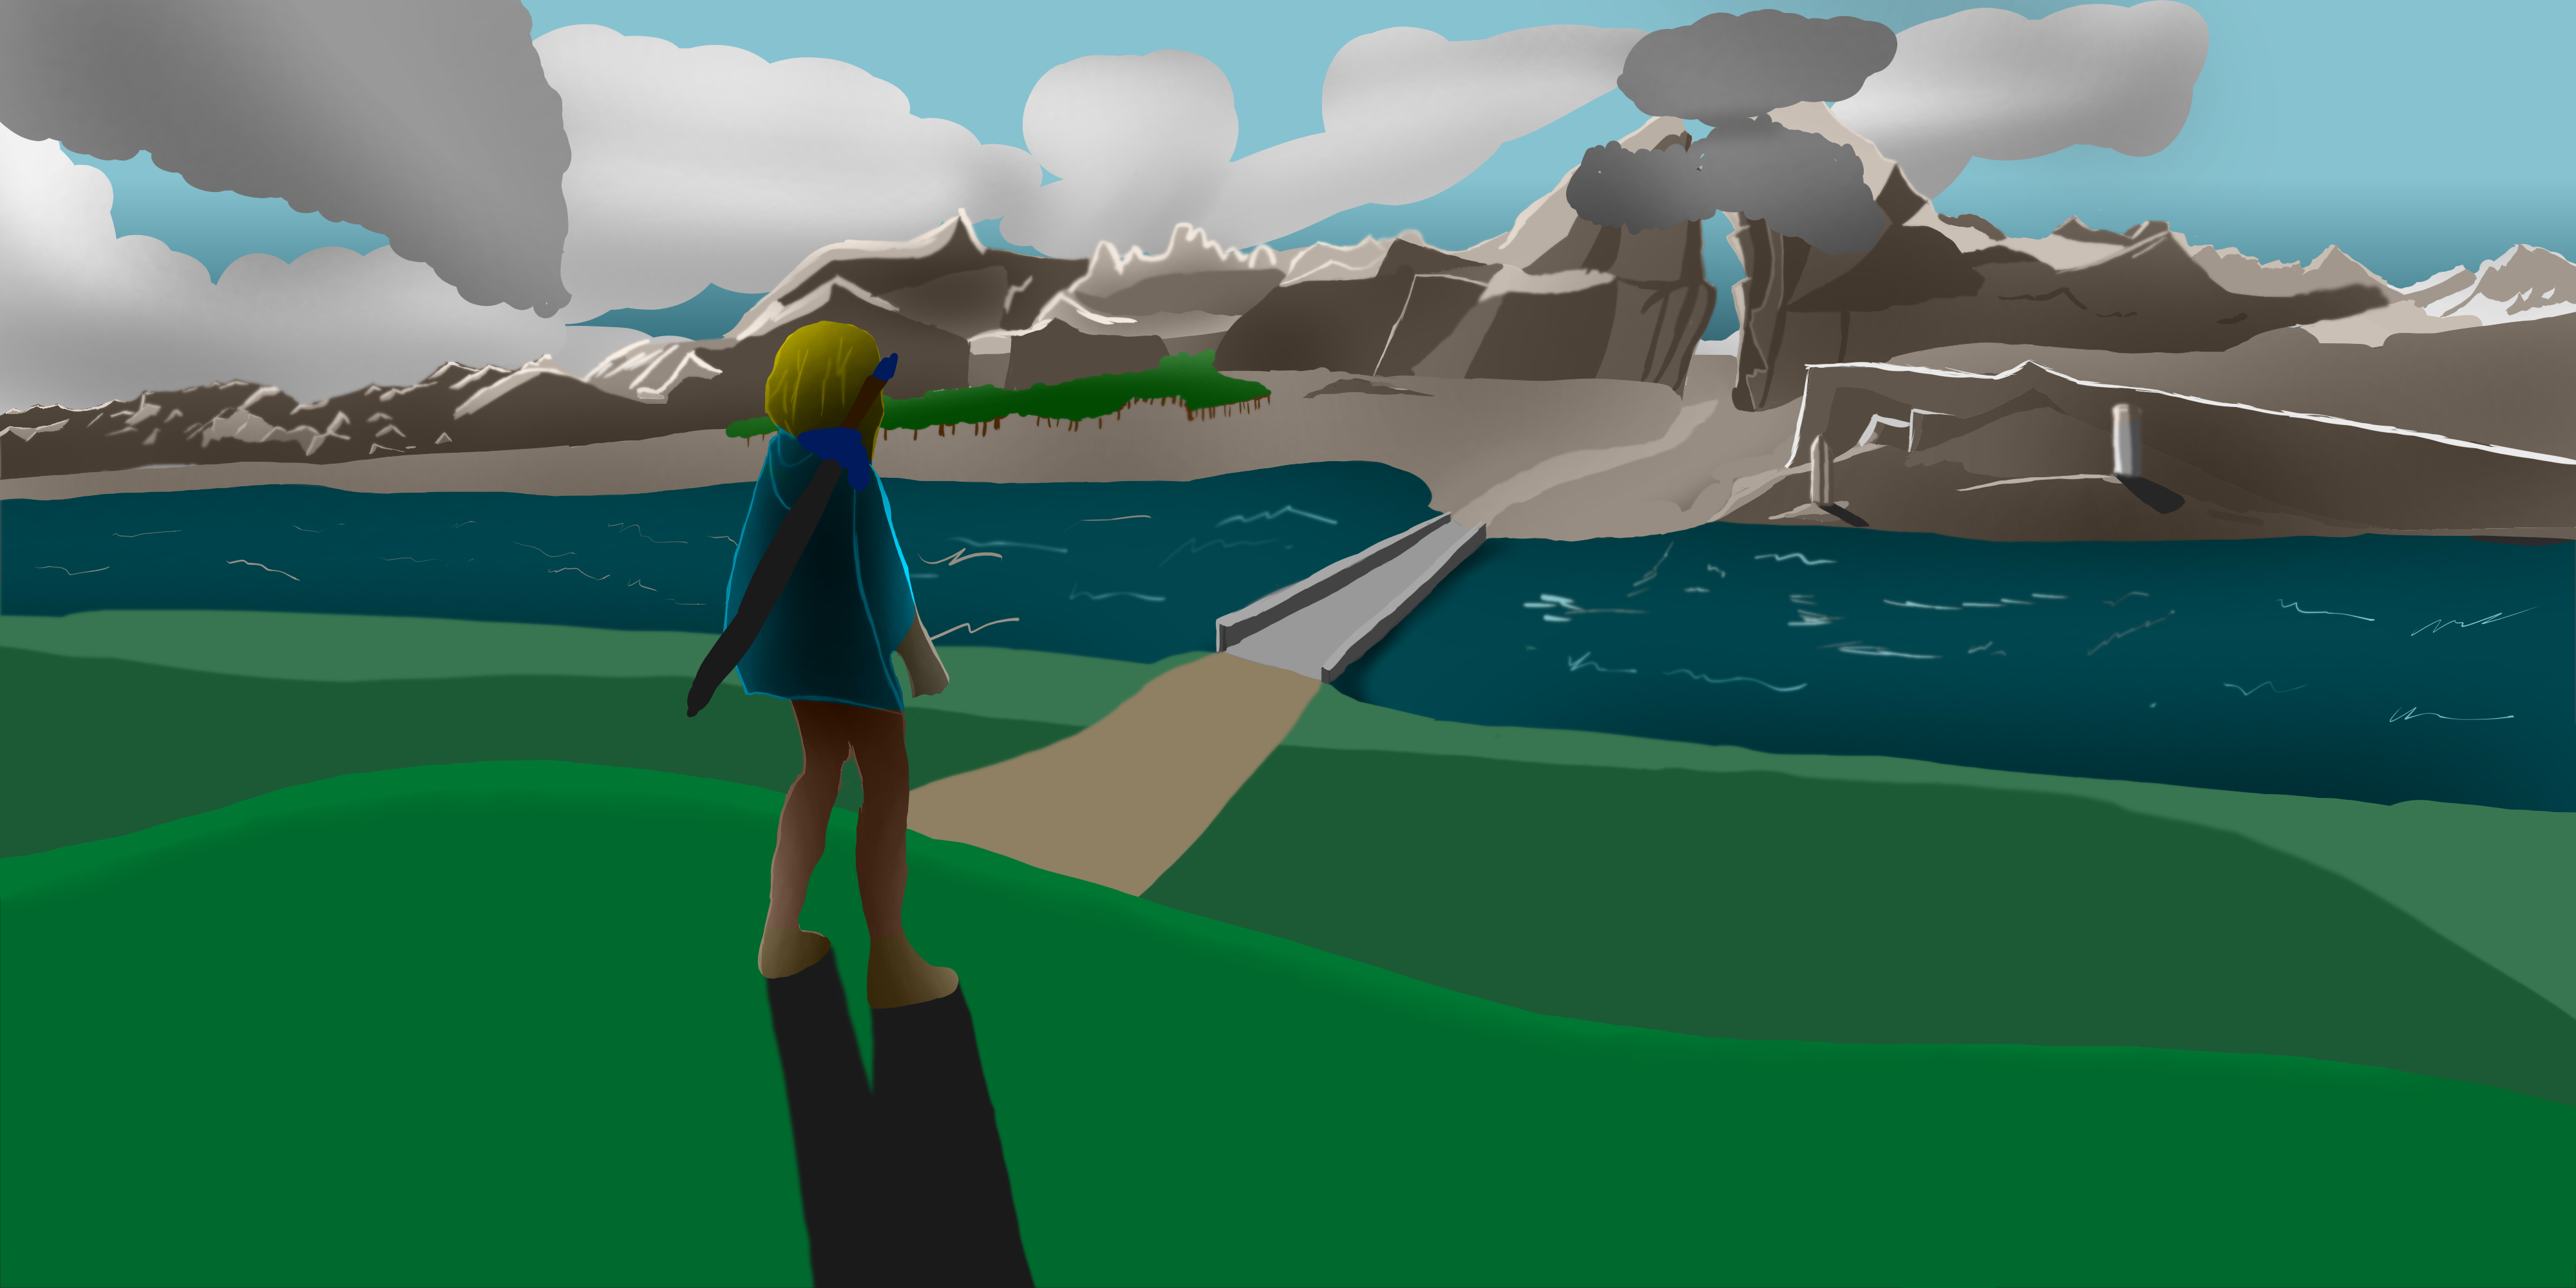
\includegraphics[width=\textwidth]{Imagenes/Fanart1/Color/III_Iteracion.png}
            \caption{Third iteration of the coloring.}
        \end{figure}

        And for the last iteration I added a warm and yellowish tone to the sky, to make it look like a sunset.\\
        \begin{figure}[H]
            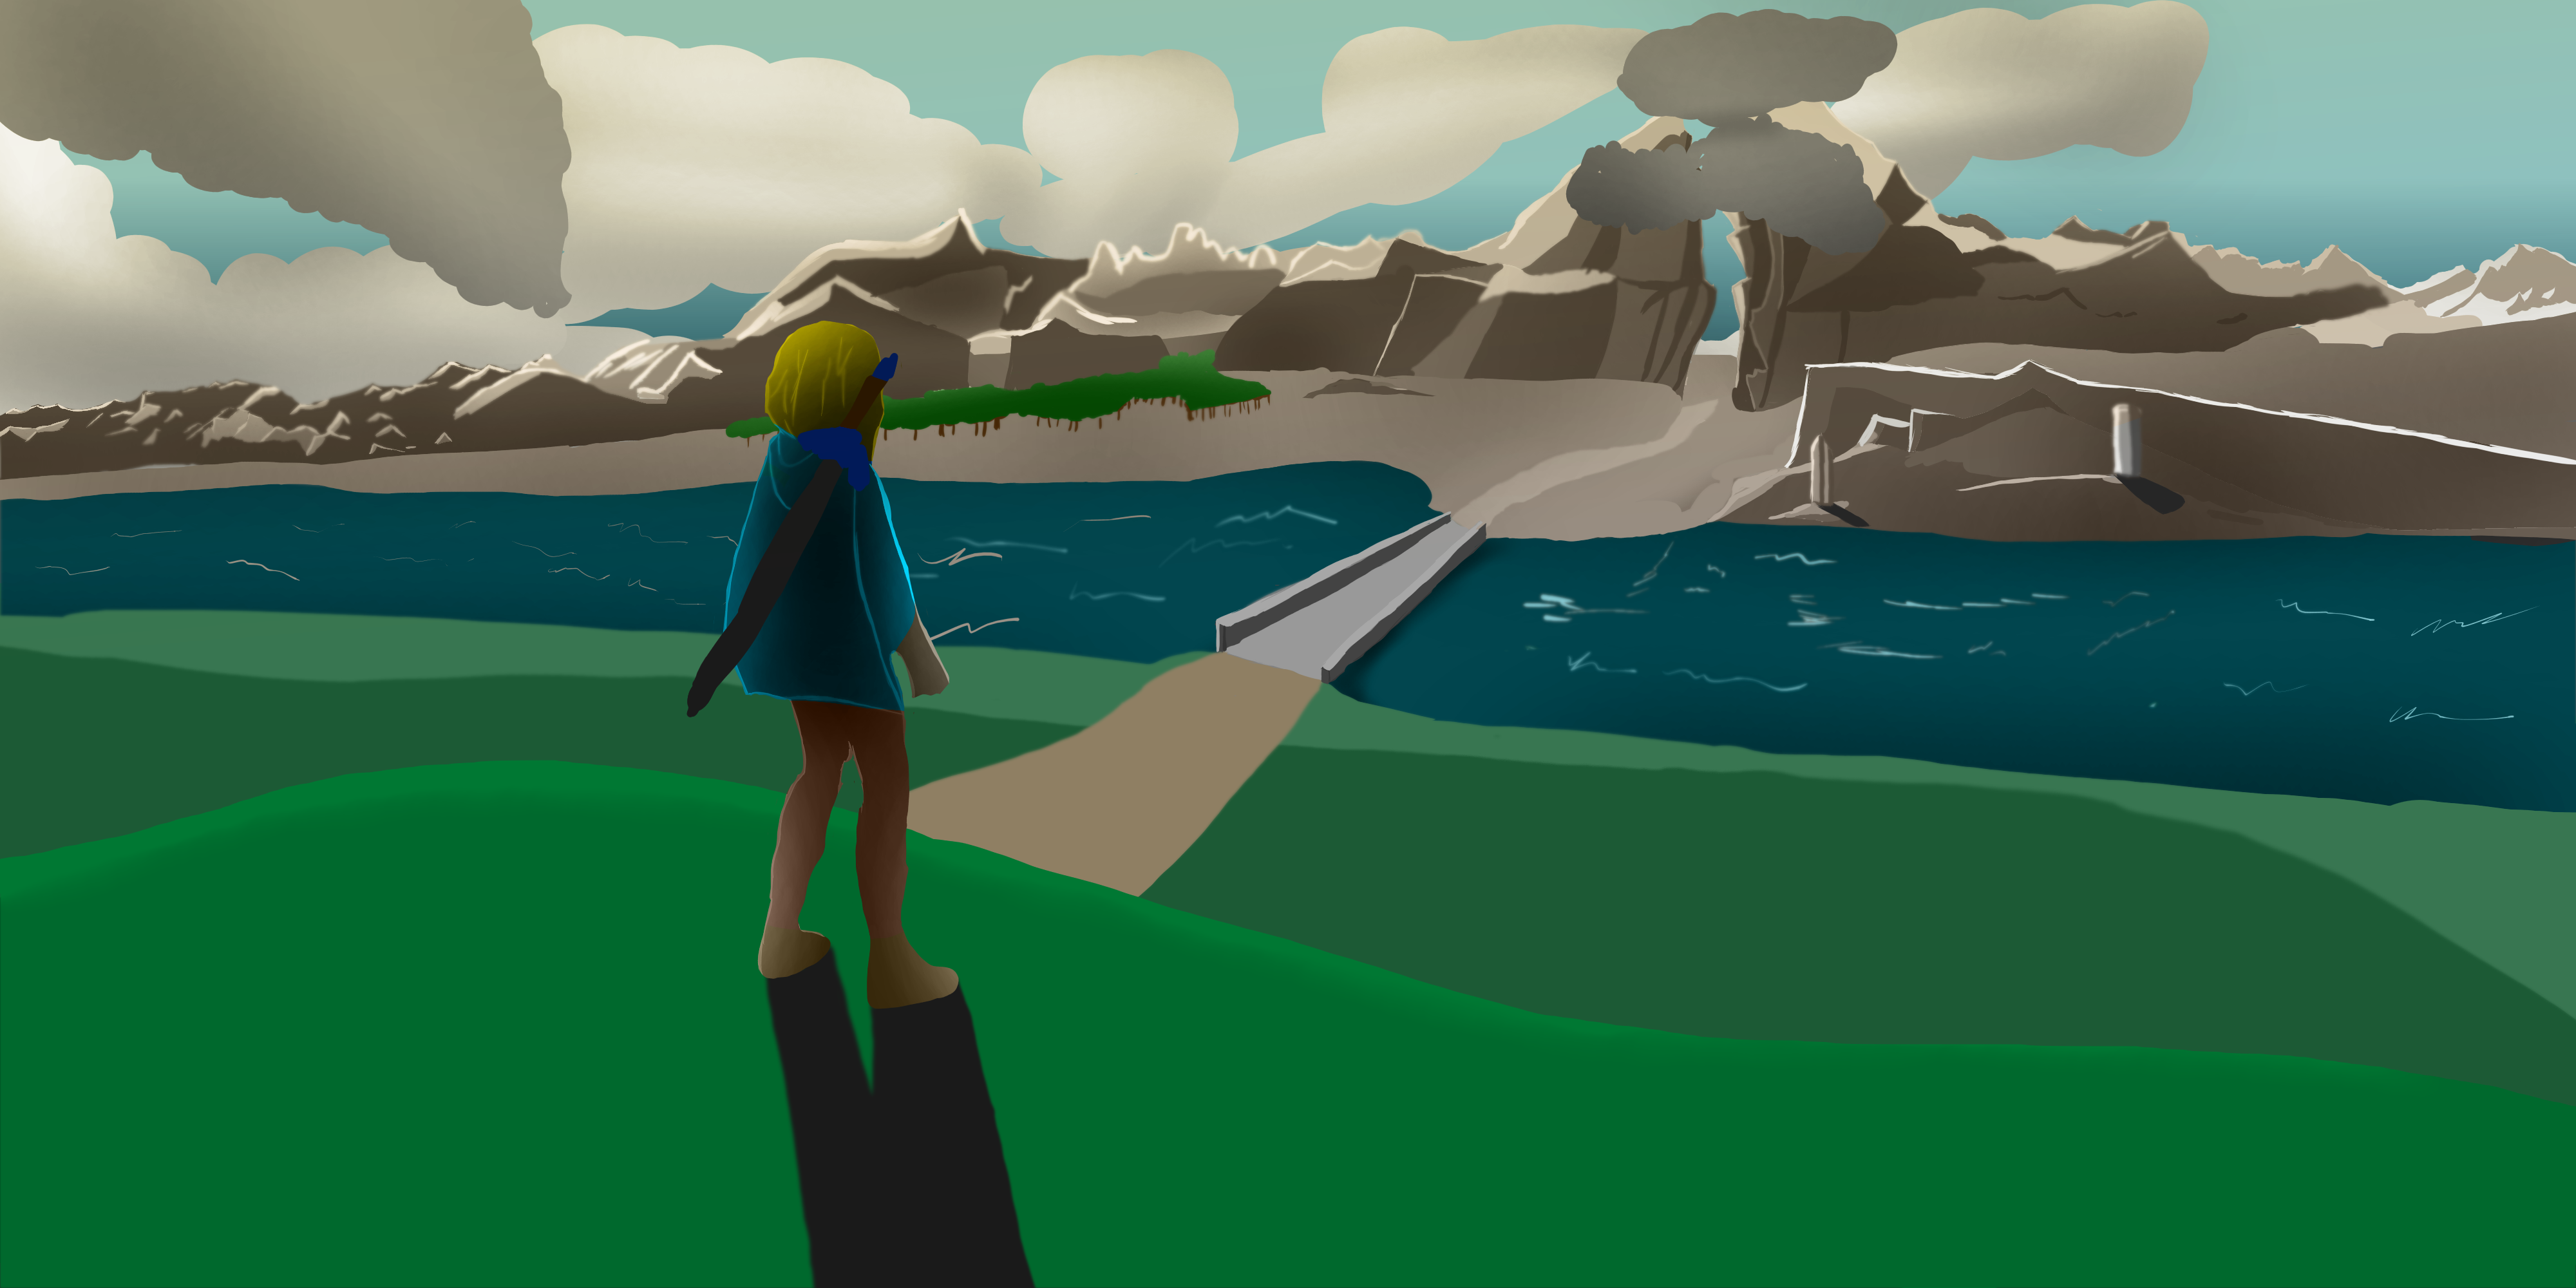
\includegraphics[width=\textwidth]{Imagenes/Fanart1/Color/IIII_Iteracion.png}
            \caption{Fourth iteration of the coloring.}
        \end{figure}
        
    \subsection{Final Result}
        The final result of the fan art is the following:
        \begin{figure}[H]
            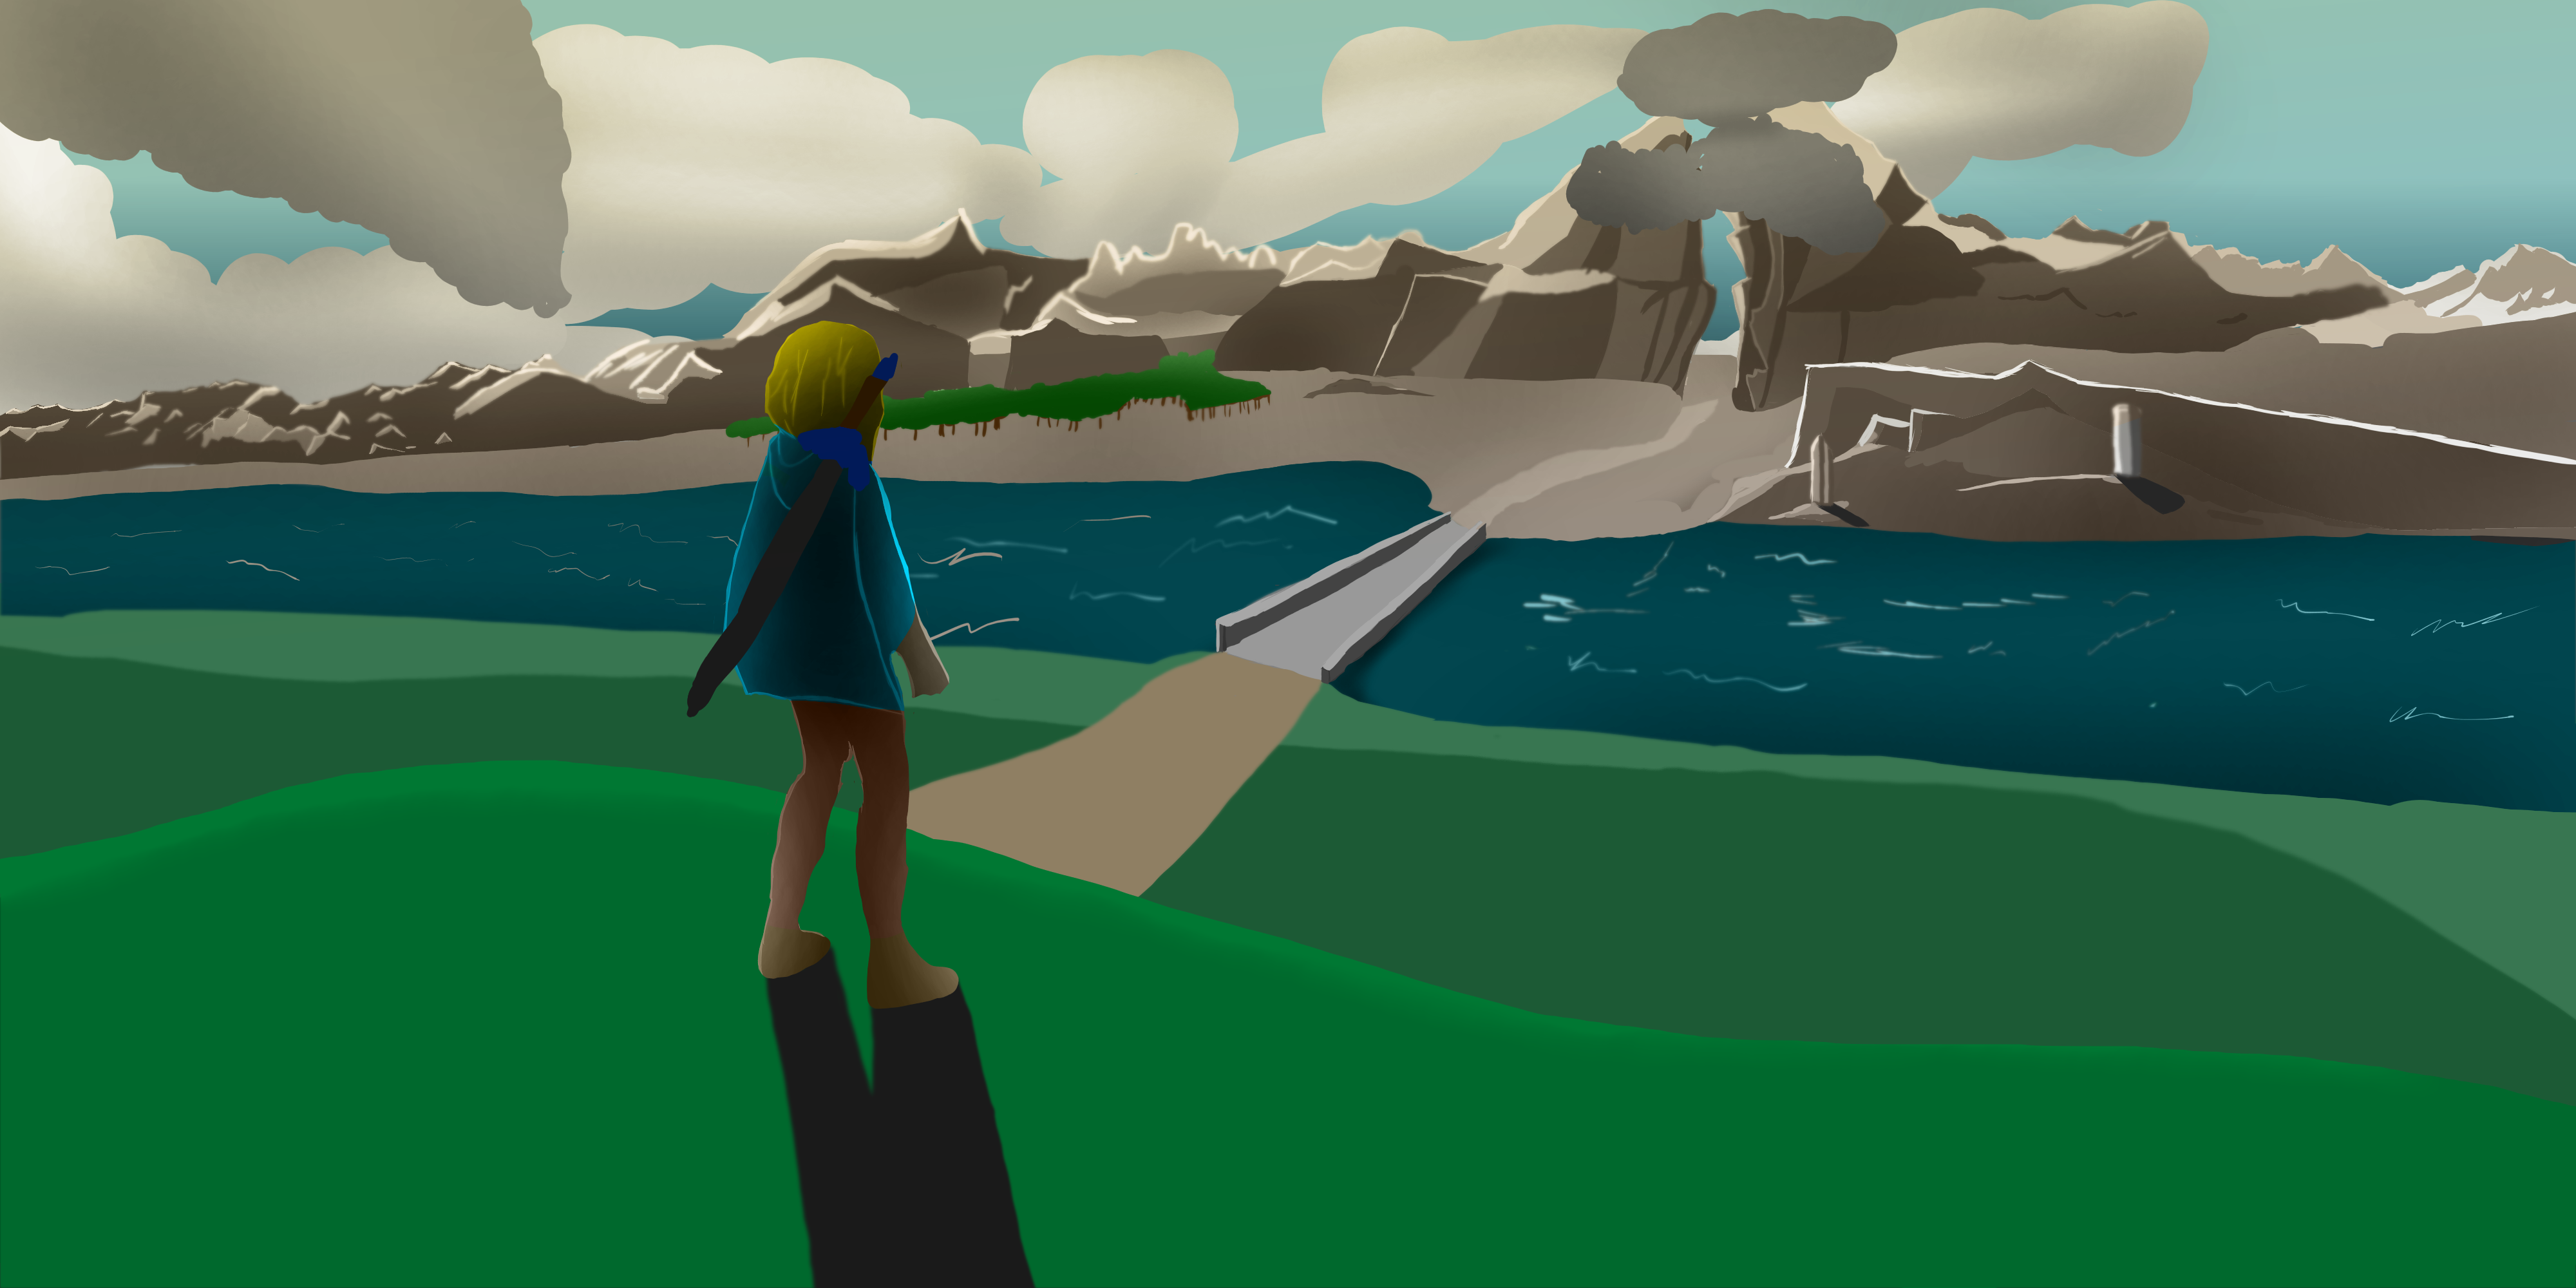
\includegraphics[width=\textwidth]{Imagenes/Fanart1/Color/IIII_Iteracion.png}
            \caption{Final result of the fan art.}
        \end{figure}
        Sadly, due to the grass looking weird when drew and colored, I decided to remove it from the final result.\\

    \subsection{Formal elements of the image}

        \subsubsection{Perspective}

            The horizon line is situated almost in the middle of the image, a little higher up. This is because the image is a landscape, and the horizon line is the line where the sky and the ground meet, which is located behind the Dueling Peaks. \\
            \begin{figure}[H]
                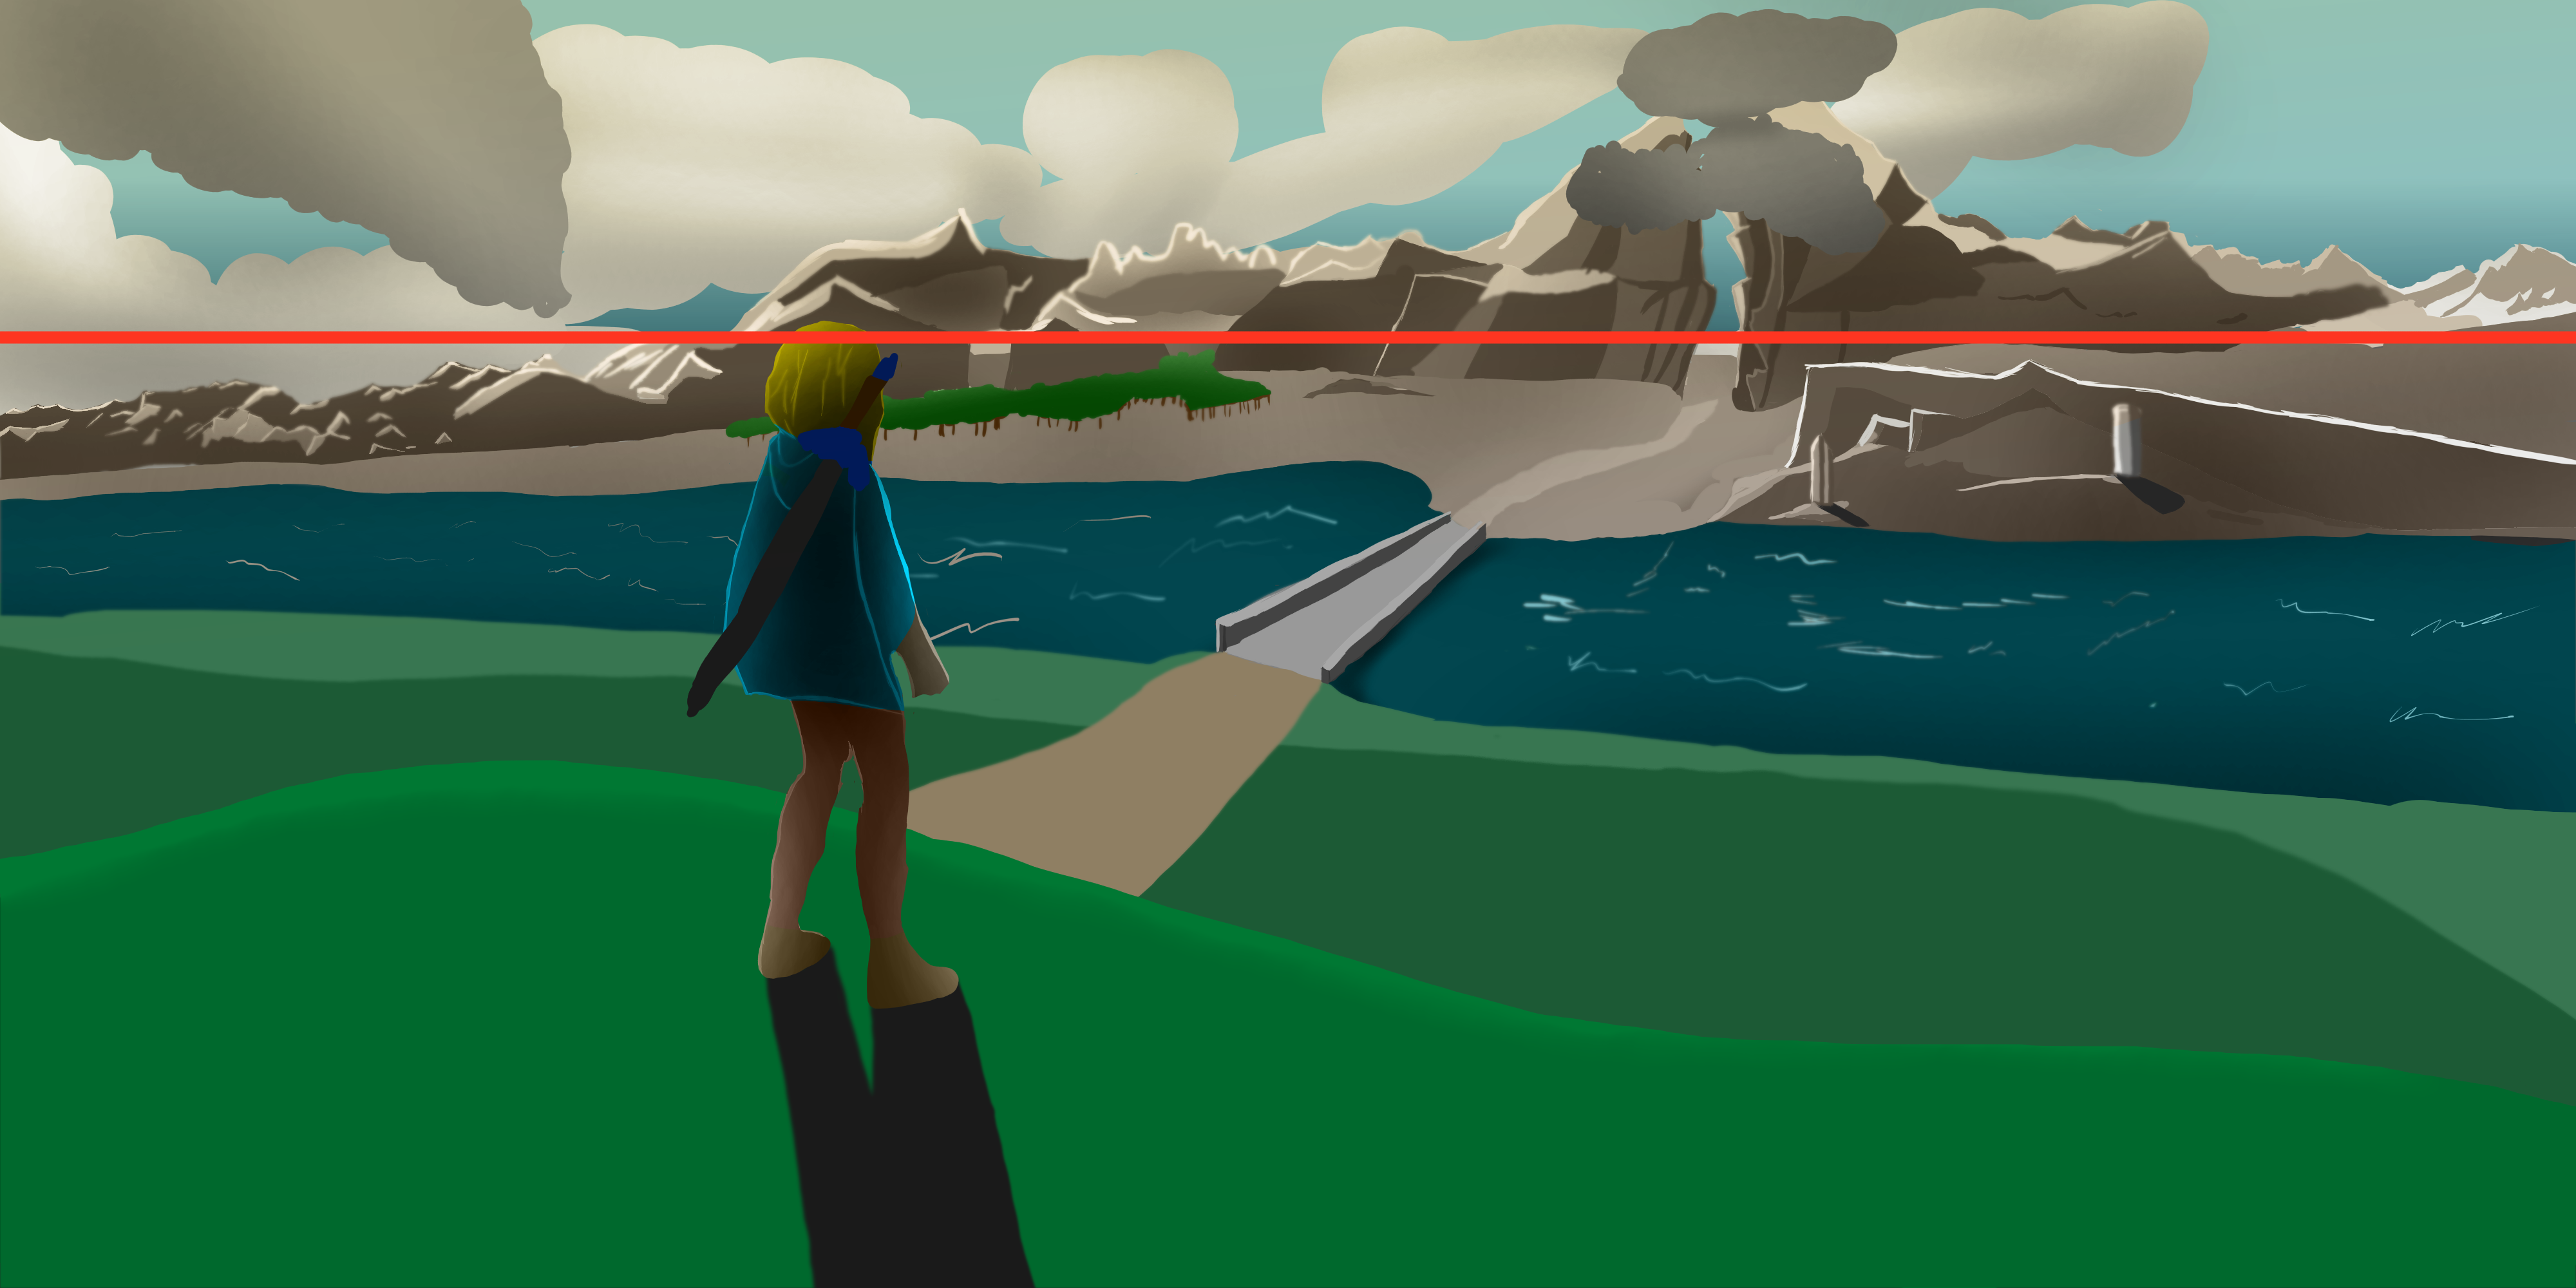
\includegraphics[width=\textwidth]{Imagenes/Fanart1/Analysis/horizonte.png}
                \caption{Horizon line of the first fan art.}
            \end{figure}

            Because the composition is a landscape, the vanishing points are unclear where it is located, so we can conclude there's no vanishing point.\\
            However, a vanishing point could be located in the middle of the Dueling Peaks, but it's not a clear one.\\
            \begin{figure}[H]
                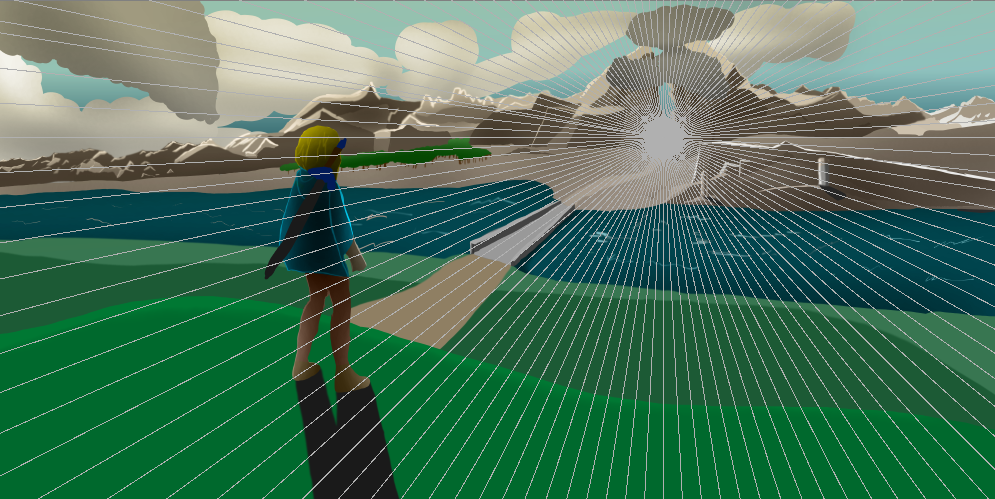
\includegraphics[width=\textwidth]{Imagenes/Fanart1/Analysis/puntofuga.png}
                \caption{Theoretical vanishing point. (using Krita's vanishing point tool)}
            \end{figure}

        \subsubsection{Composition}

            The rule of thirds is used extensively on this image. The two left thirds are occupied by Zelda and the top right third is focused on the middle of the Dueling Peaks.\\
            \begin{figure}[H]
                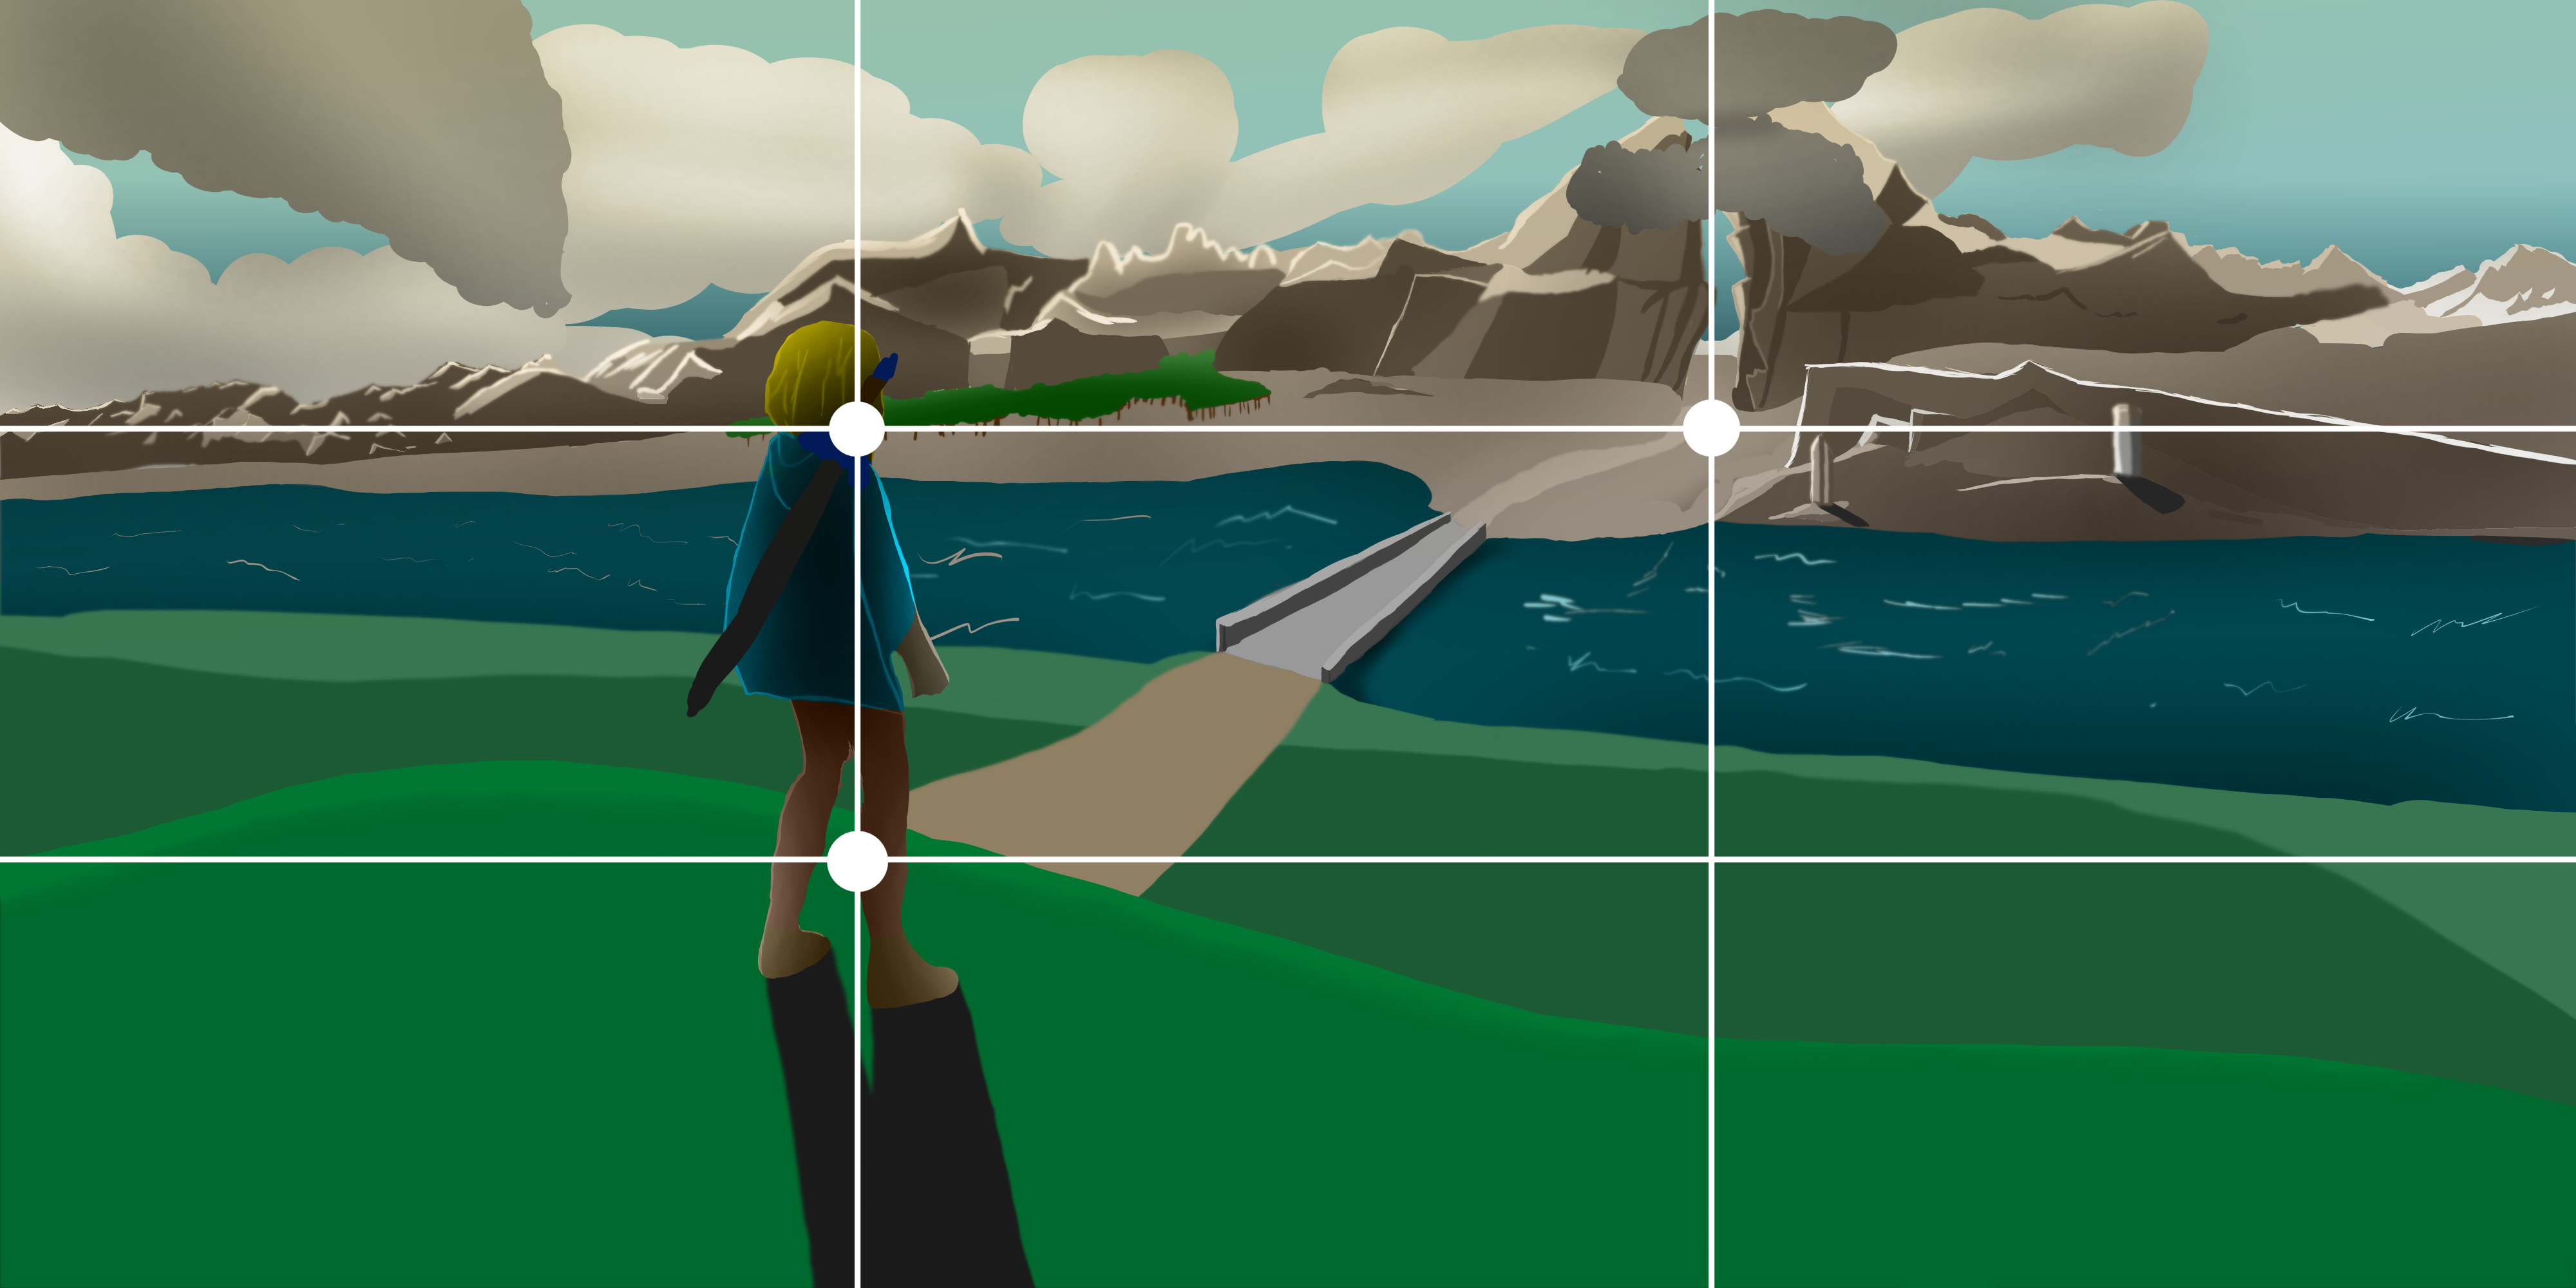
\includegraphics[width=\textwidth]{Imagenes/Fanart1/Analysis/reglatercios.png}
                \caption{Rule of Thirds of the first fan art.}
            \end{figure}

            The image has a clear path of how the spectator sees the images. It starts at Zelda, moving to the bridge which its shapes carriers the eye to the Dueling Peaks, to end it on the hills at the right.\\
            \begin{figure}[H]
                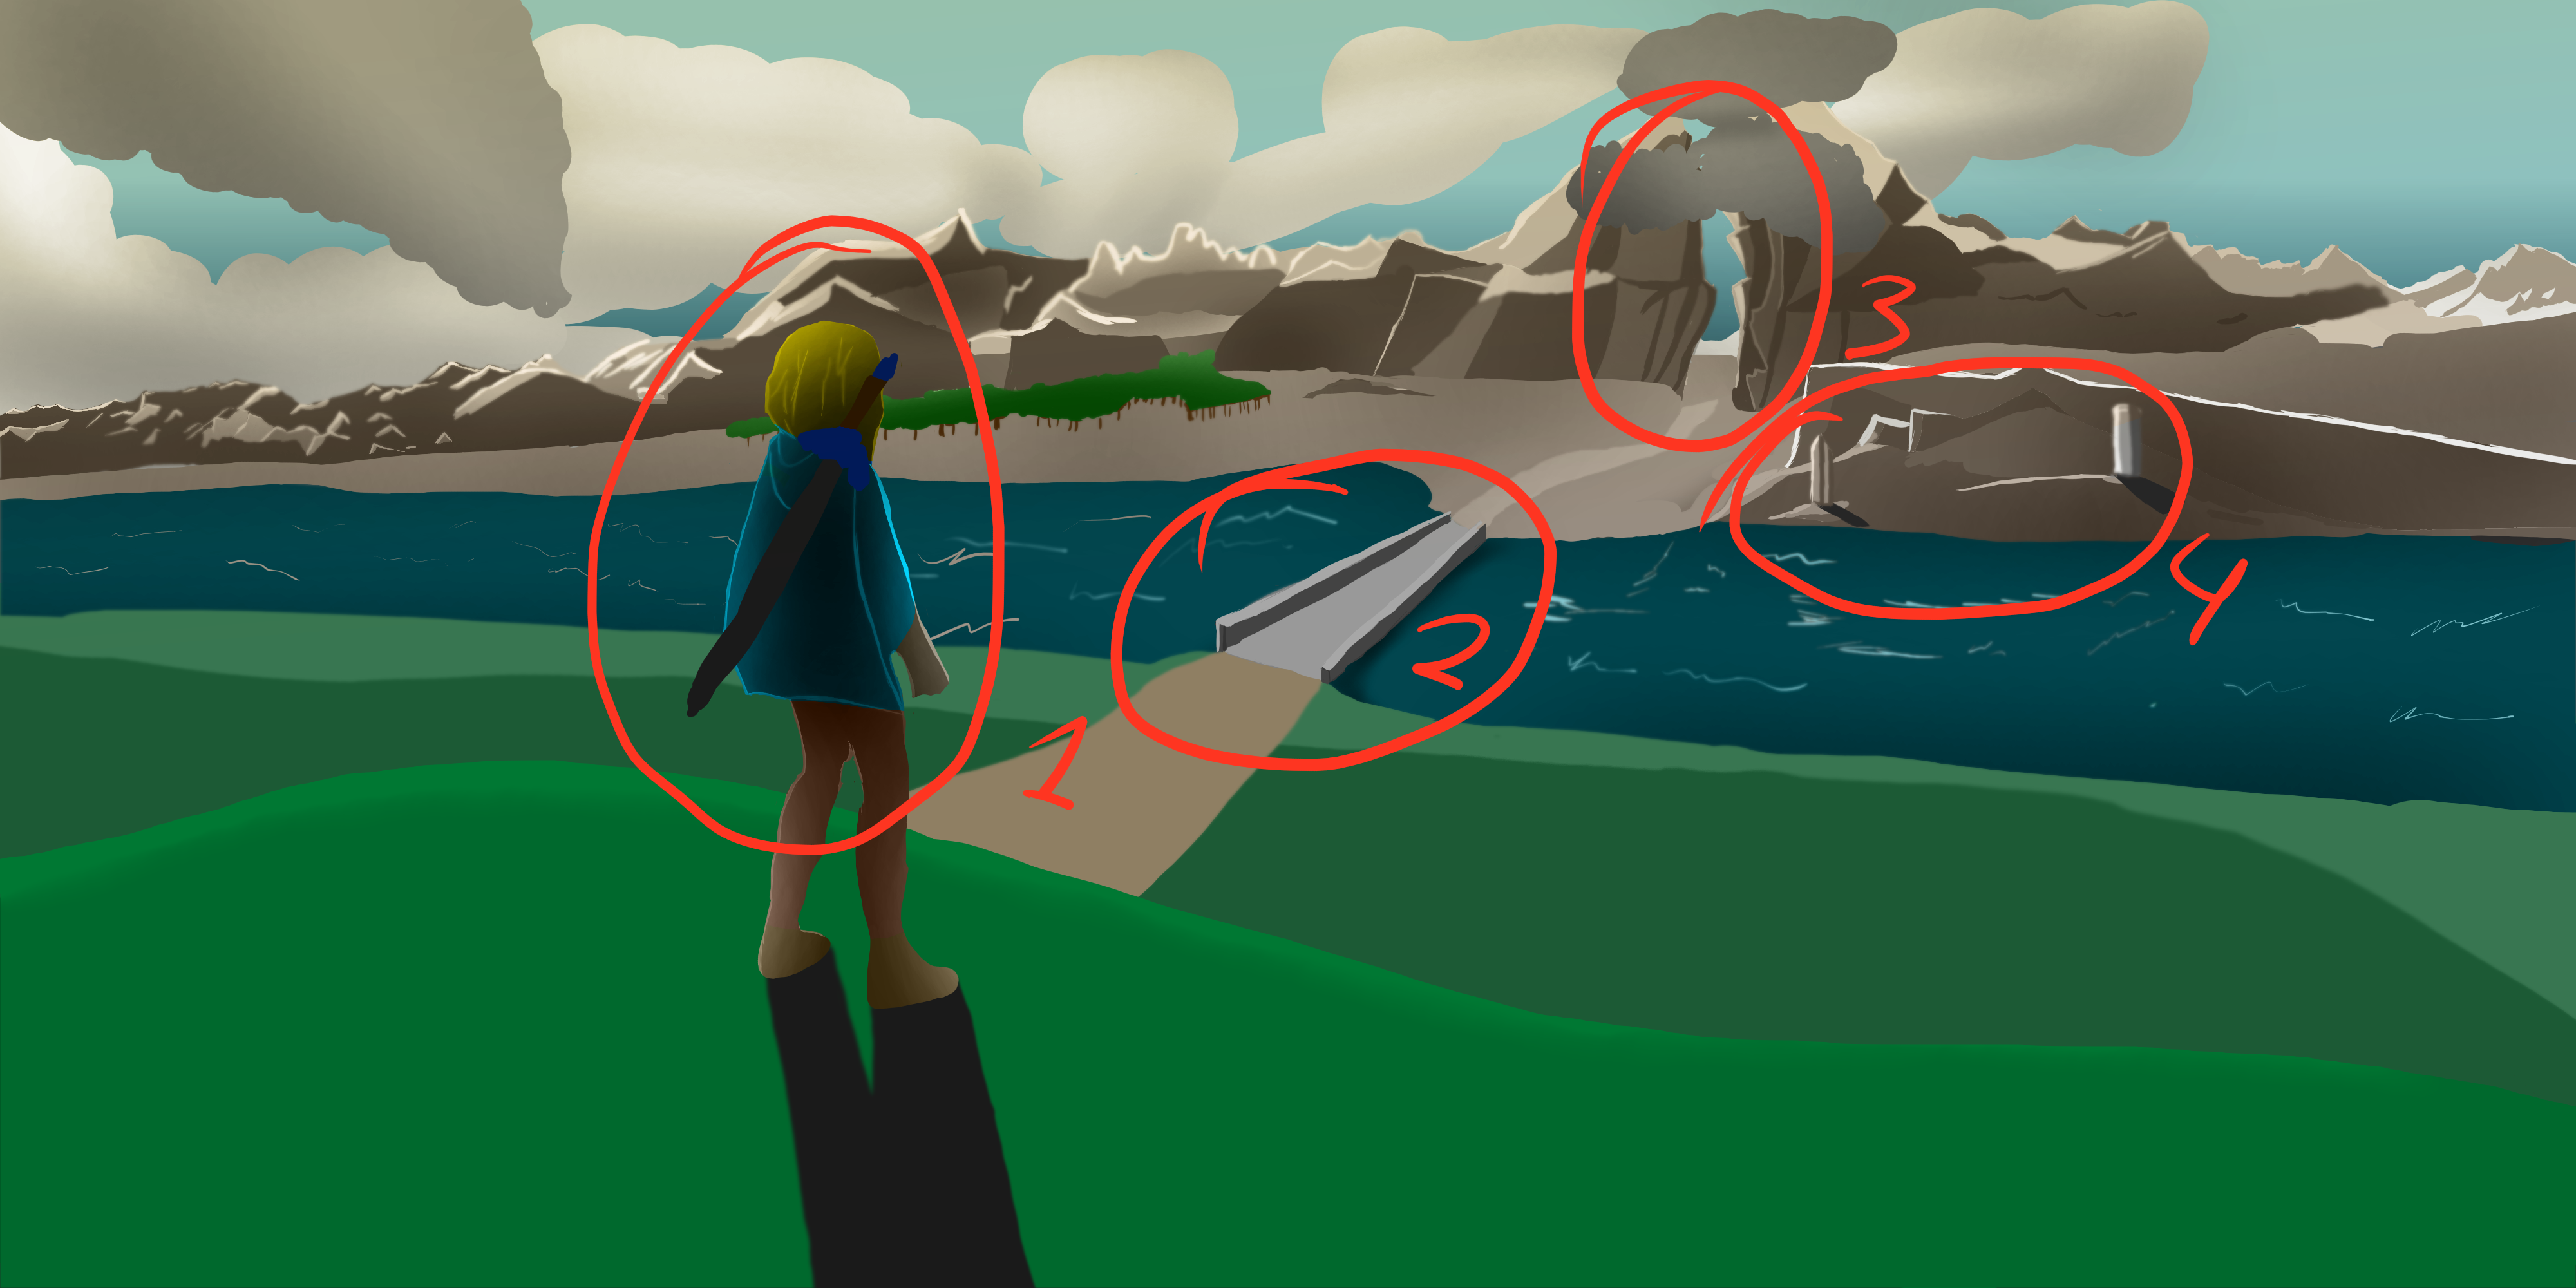
\includegraphics[width=\textwidth]{Imagenes/Fanart1/Analysis/puntosinteres.png}
                \caption{Interest Points of the first fan art.}
            \end{figure}

            This image is thought to the ground up to guide the spectator to the main point of the image, the middle of the Dueling Peaks.\\
            The path begins at Zelda and continues on to the bridge, which is accompanied by the river and the hills at both sides, compressing the path.\\
            The clouds and the hills surrounding the Dueling Peaks are also used to guide the spectator to the middle of the image.\\
            \begin{figure}[H]
                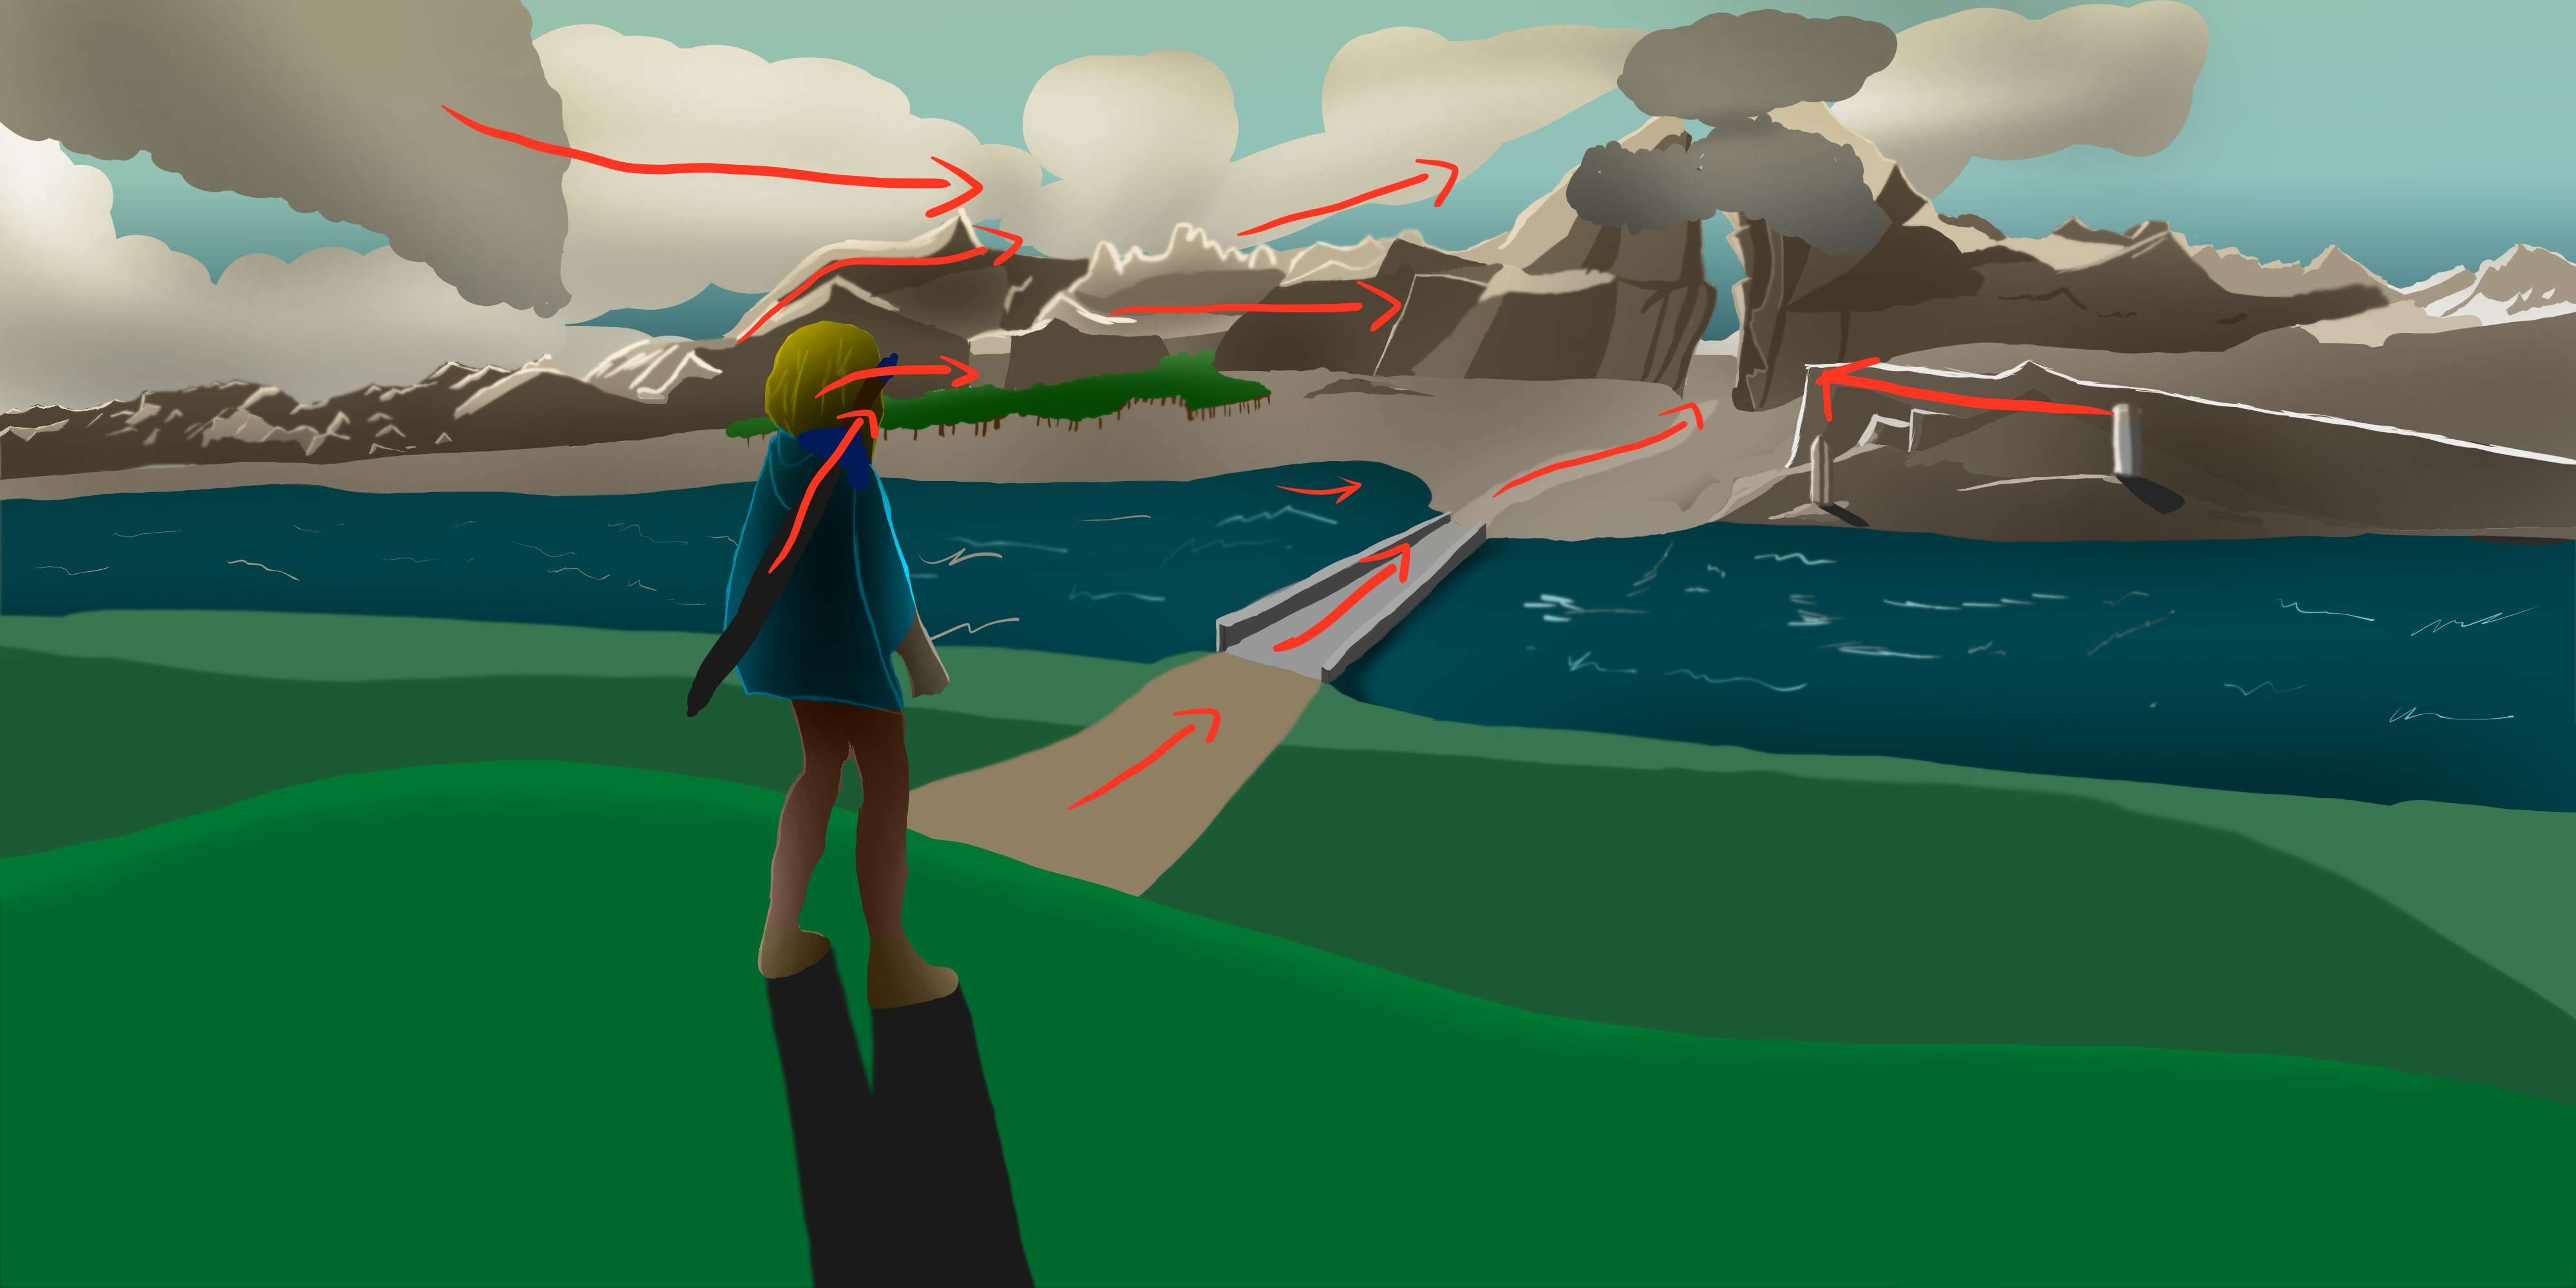
\includegraphics[width=\textwidth]{Imagenes/Fanart1/Analysis/recorridovisual.png}
                \caption{Visual Paths.}
            \end{figure}

            The image is not symmetrical and not balanced. The image is not balanced because the Dueling Peaks are not in the middle of the image and Zelda is occupying most of the left part of the image.\\
            \begin{figure}[H]
                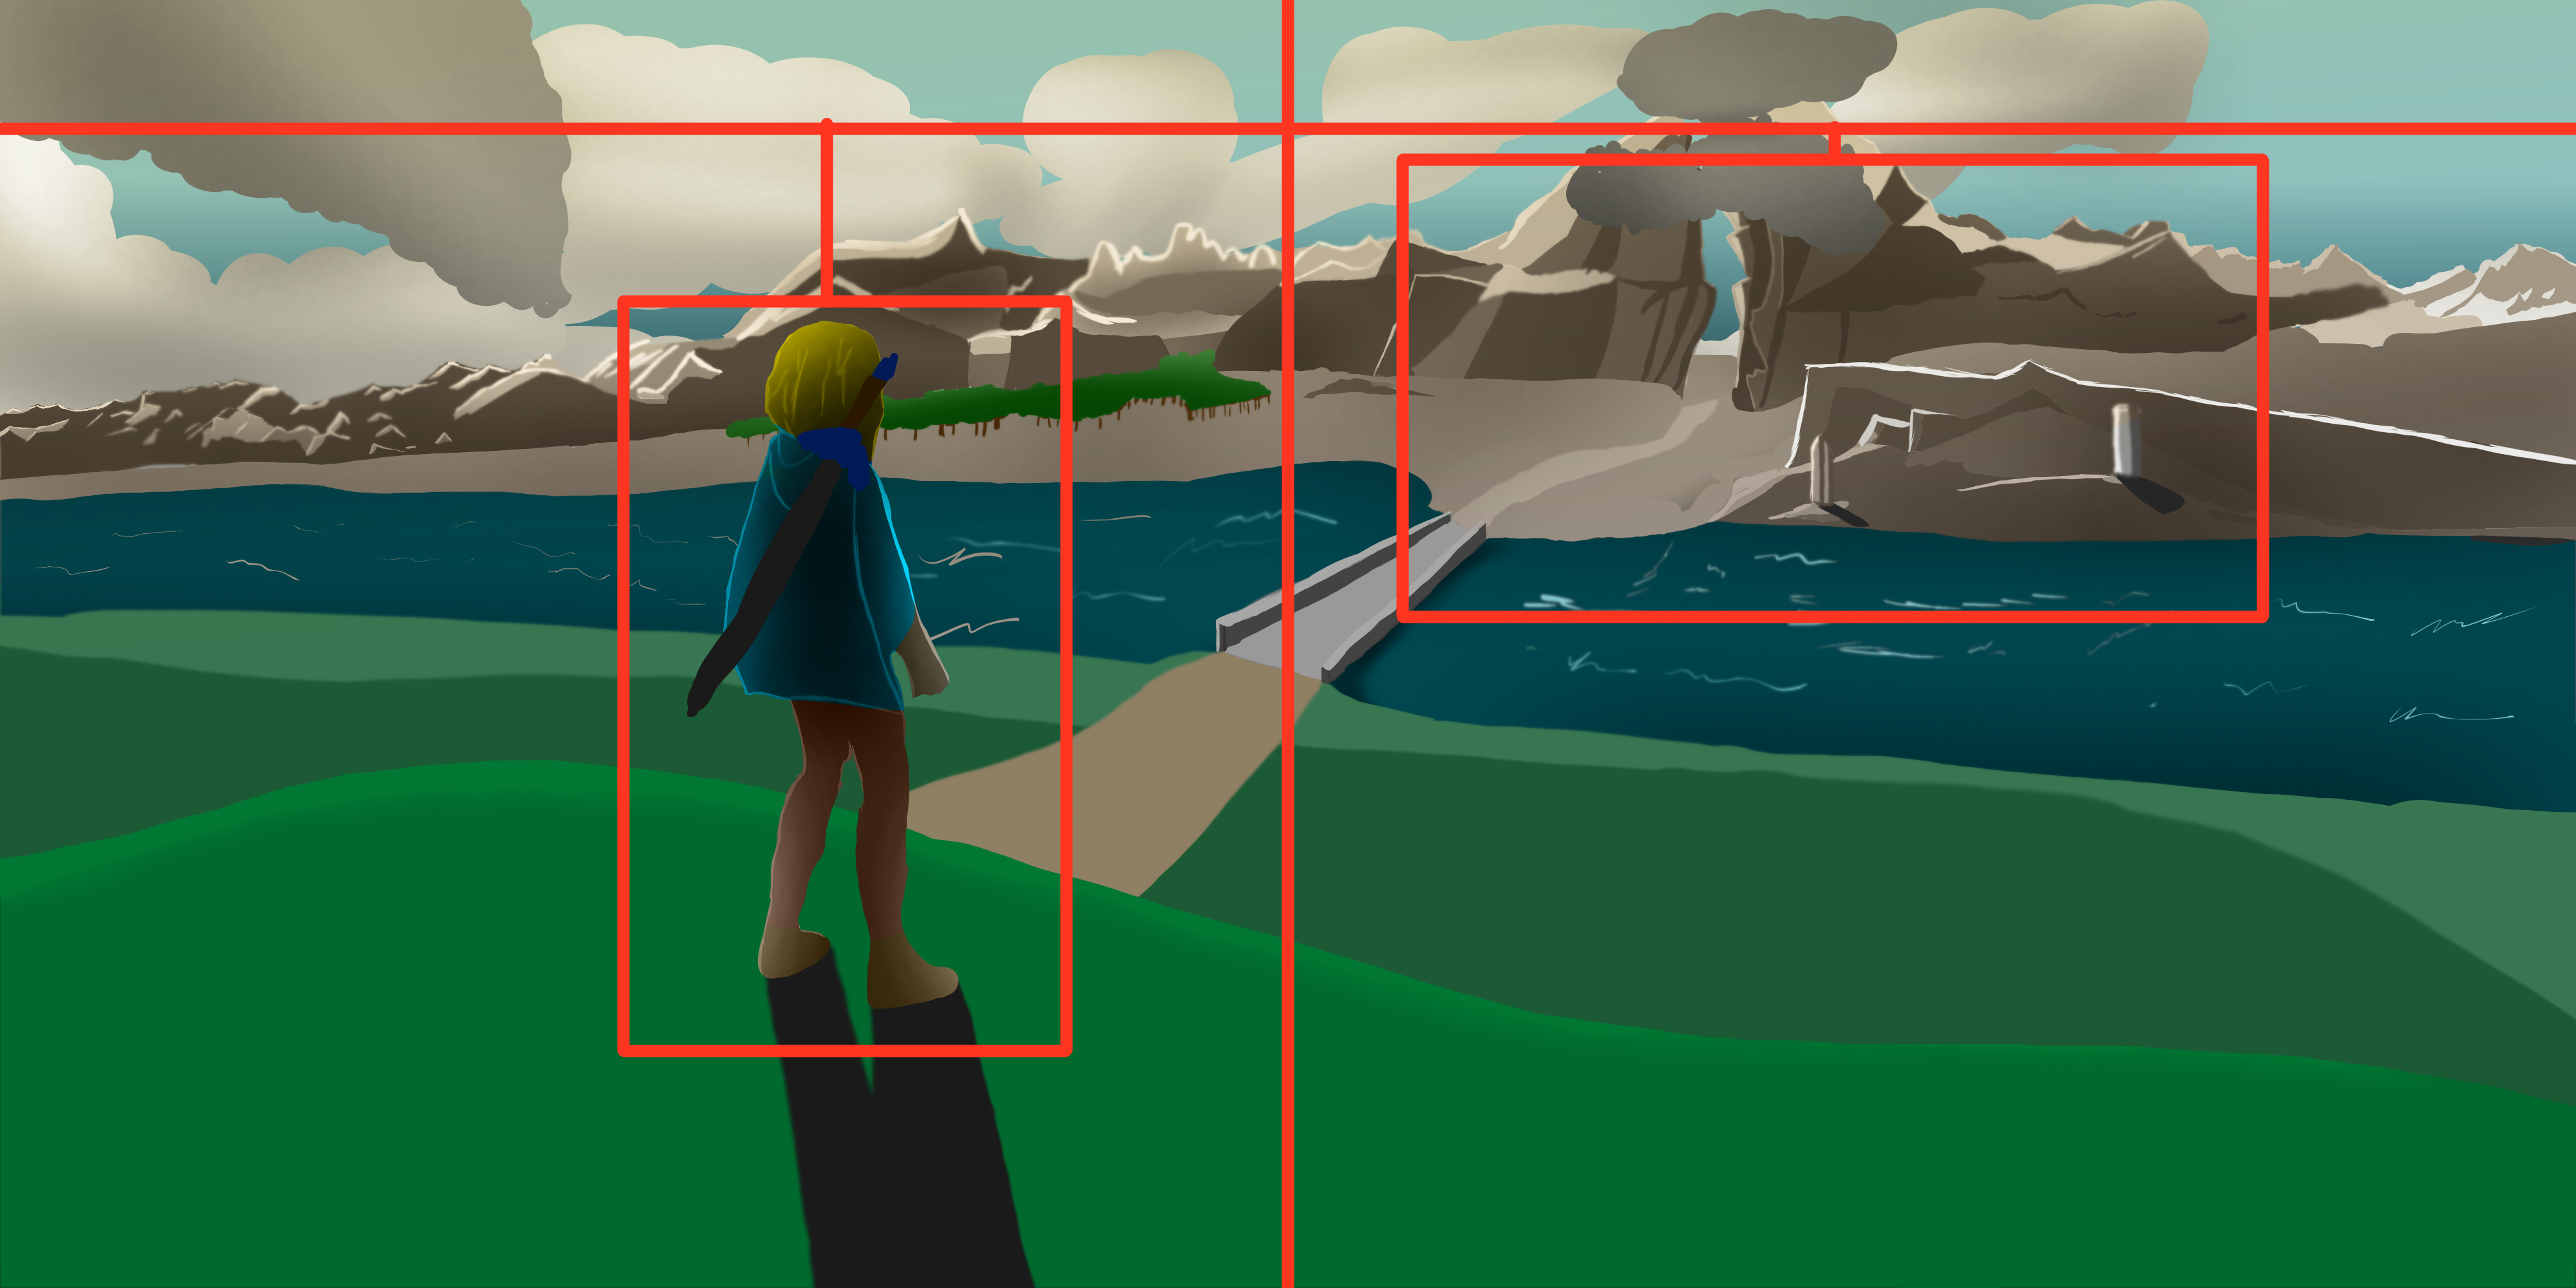
\includegraphics[width=\textwidth]{Imagenes/Fanart1/Analysis/balanza.png}
                \caption{Weight Scaling of the first fan art.}
            \end{figure}

        \subsubsection{Chiaroscuro}

            The chiaroscuro represents how the image is structured in various zones, which is clearly represented in the image.\\
            To separate this zones, I used darkness to represent this, instead of making more light zones, I used white contours around the borders of what I wanted to separate.\\
            \begin{figure}[H]
                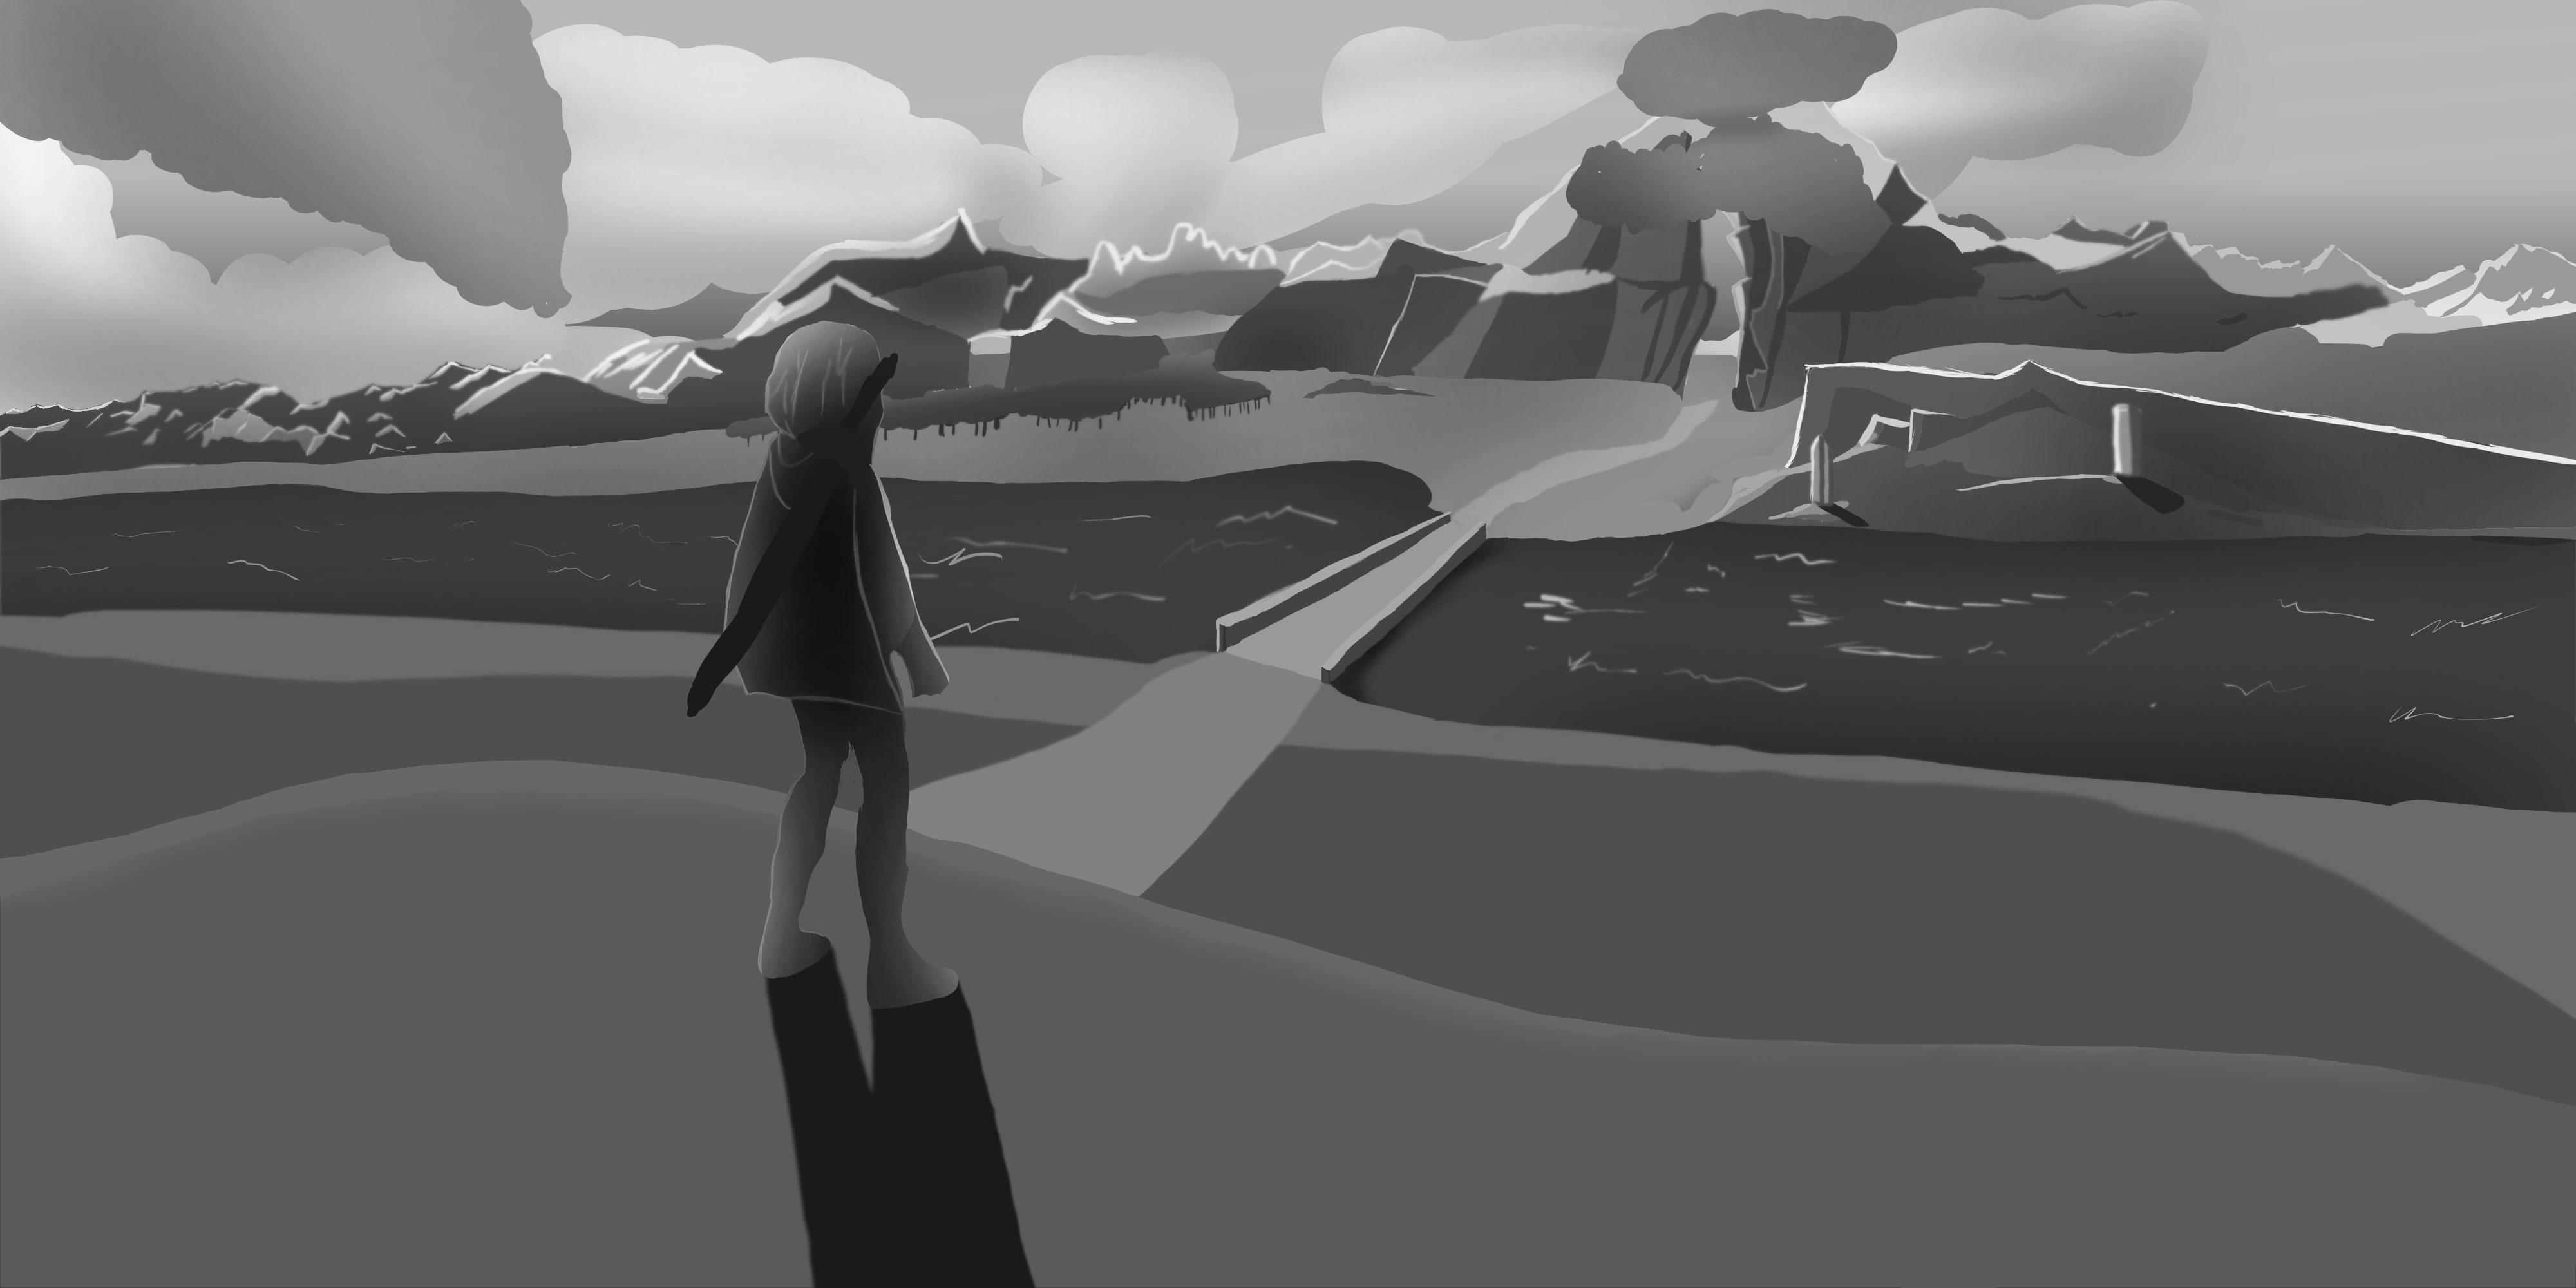
\includegraphics[width=\textwidth]{Imagenes/Fanart1/Analysis/claroscuro.png}
                \caption{Chiaroscuro of the first fan art.}
            \end{figure}

            If we pixelize the chiaroscuro, we can see even more clearly how the image is structured.\\
            \begin{figure}[H]
                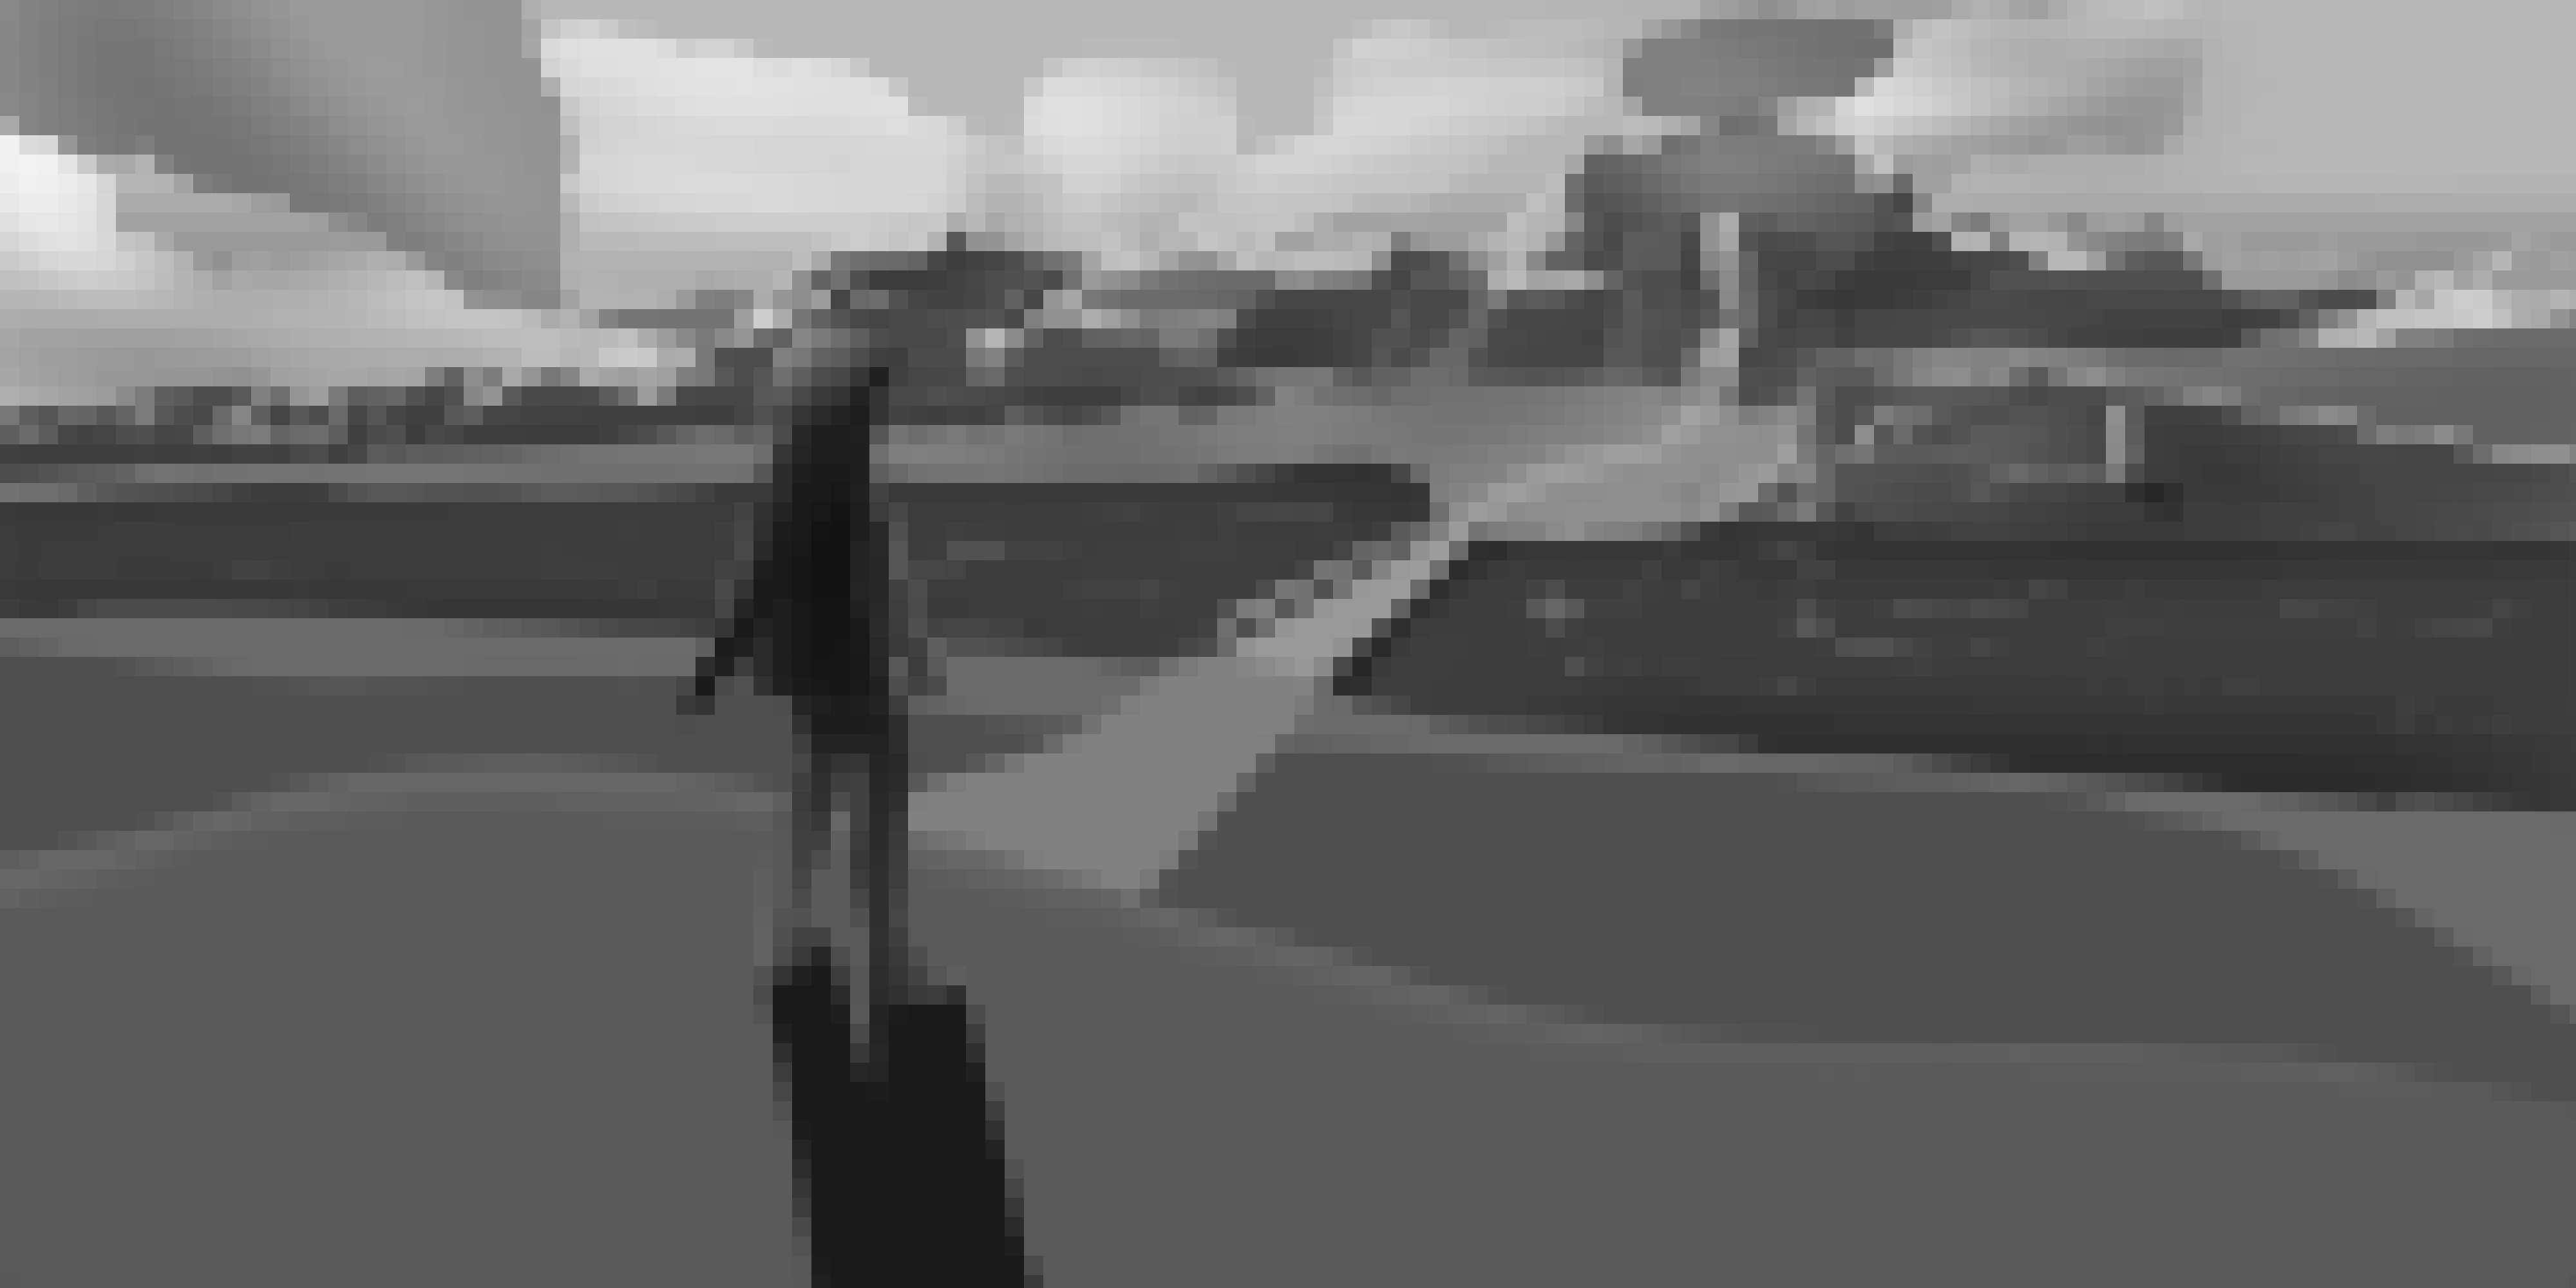
\includegraphics[width=\textwidth]{Imagenes/Fanart1/Analysis/pixel.png}
                \caption{Pixelizated Chiaroscuro of the first fan art.}
            \end{figure}

            And this is how the lights are represented in the image.
            The light is represented by the sun, which is located at the top left of the image, and covers the image with a yellowish tone.\\
            \begin{figure}[H]
                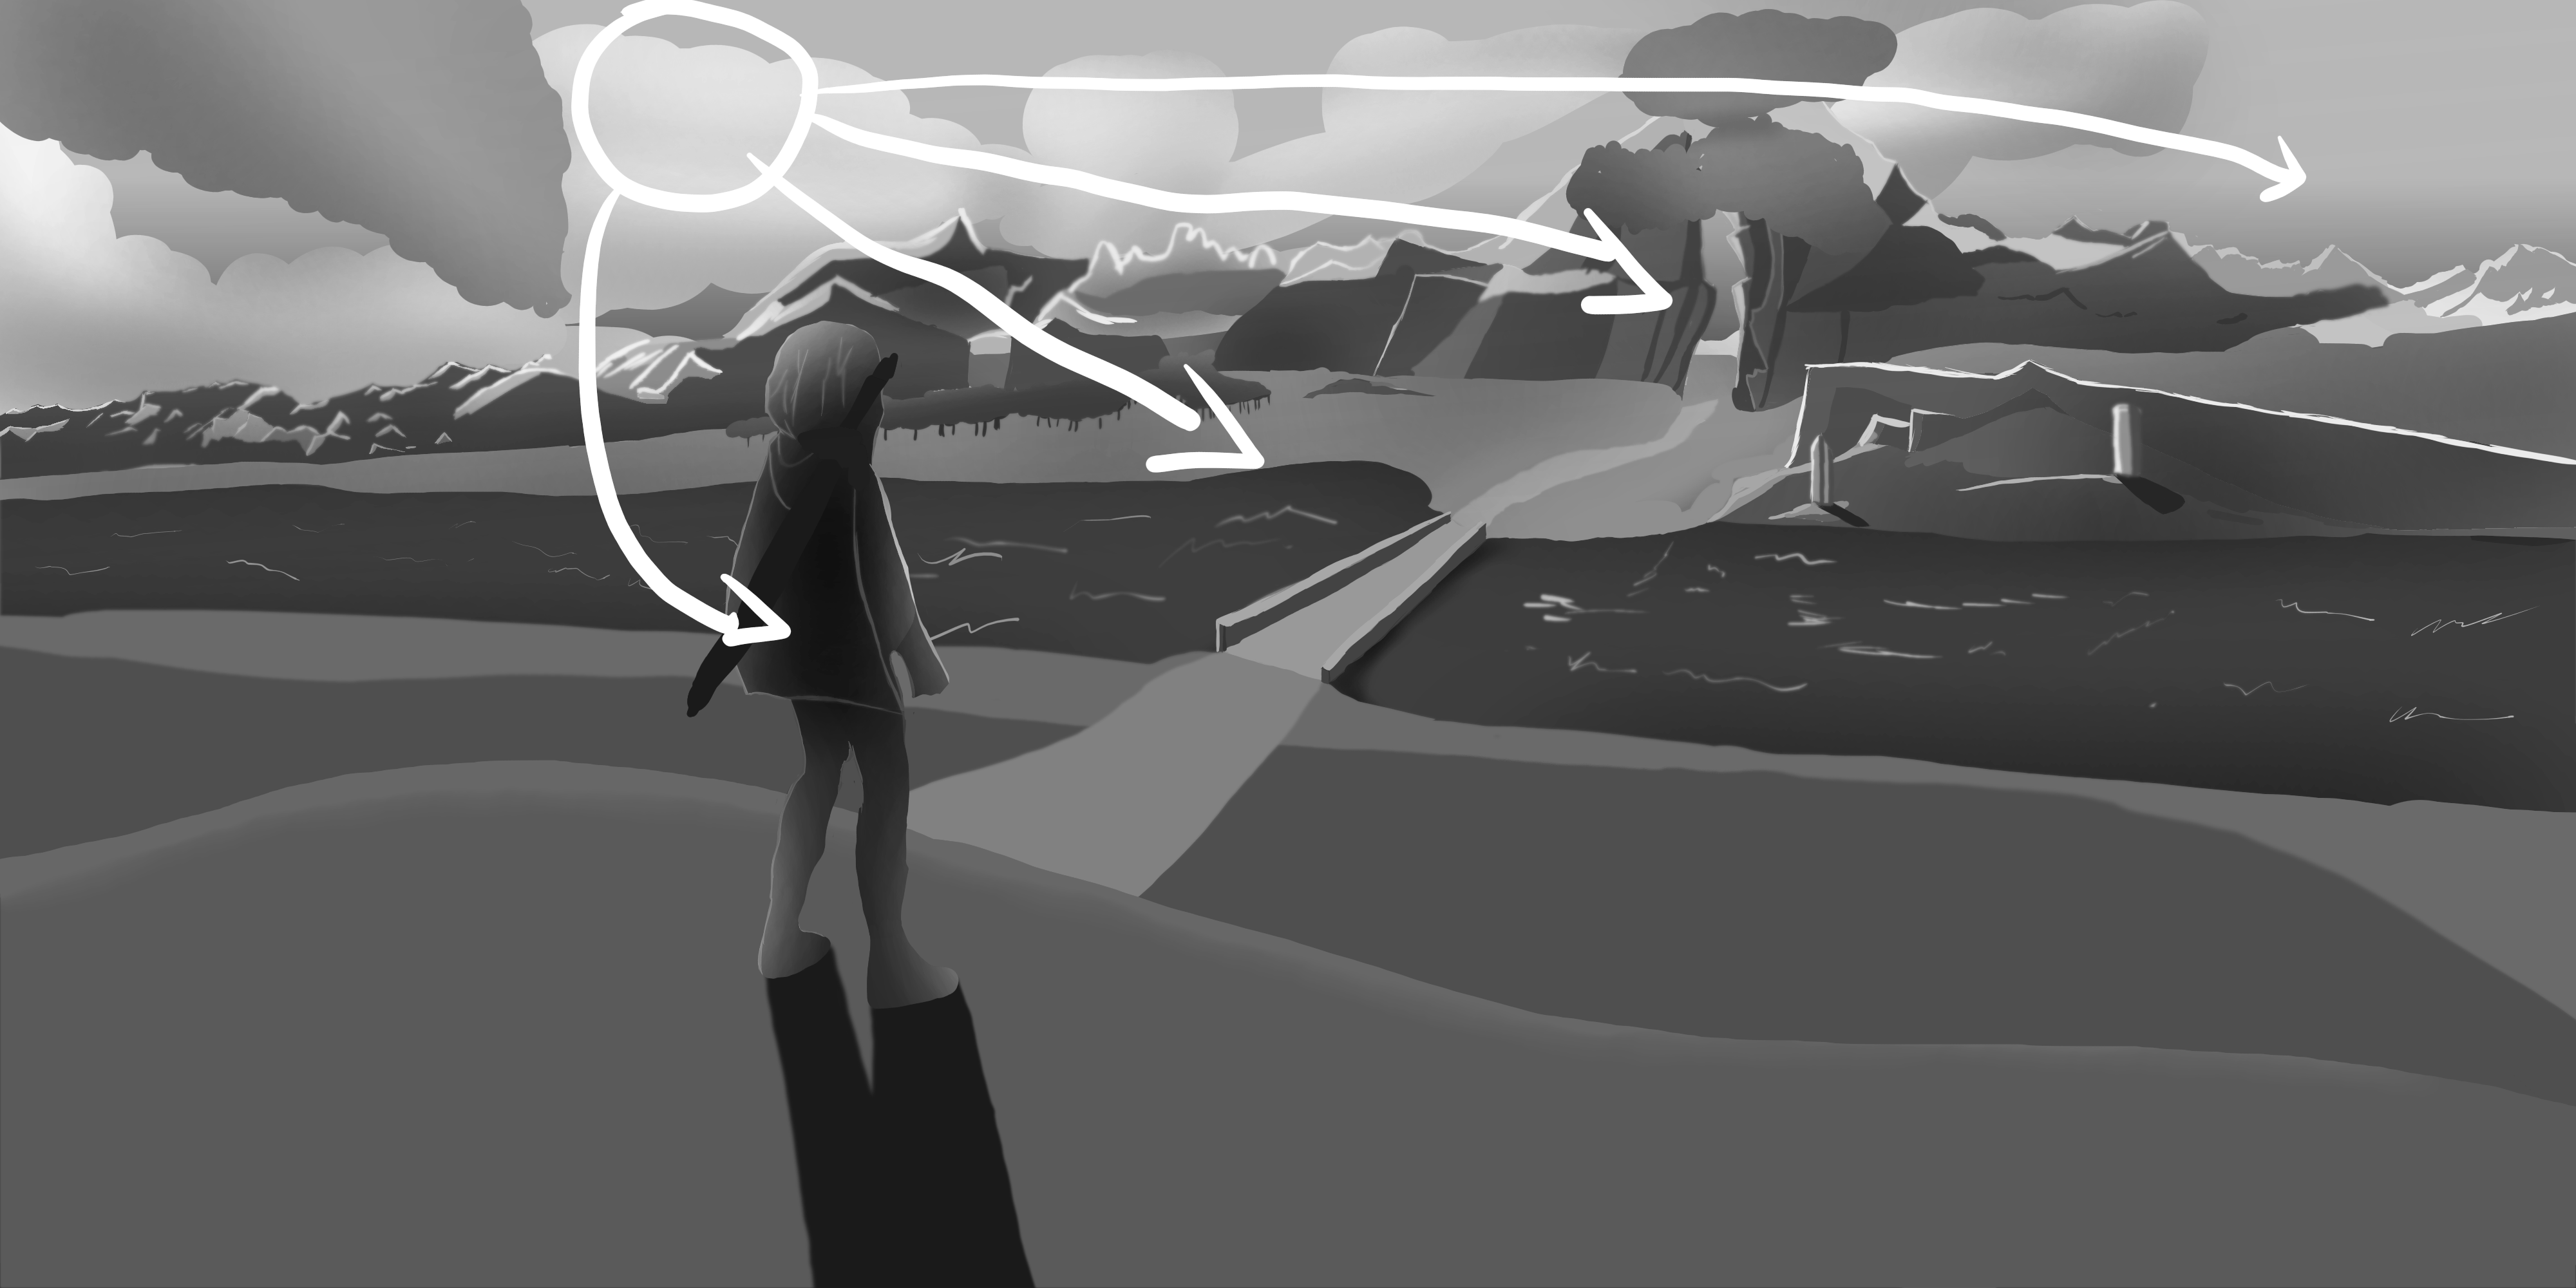
\includegraphics[width=\textwidth]{Imagenes/Fanart1/Analysis/recorridoluz.png}
                \caption{Light Paths of the first fan art.}
            \end{figure}

        \subsubsection{Color}

            The color palette is composed by various colors, ranging from the yellowish tone of the sun, to the blue of the sky and Zelda, the green of the grass and the brown used on the mountains and the plains.\\
            \begin{figure}[H]
                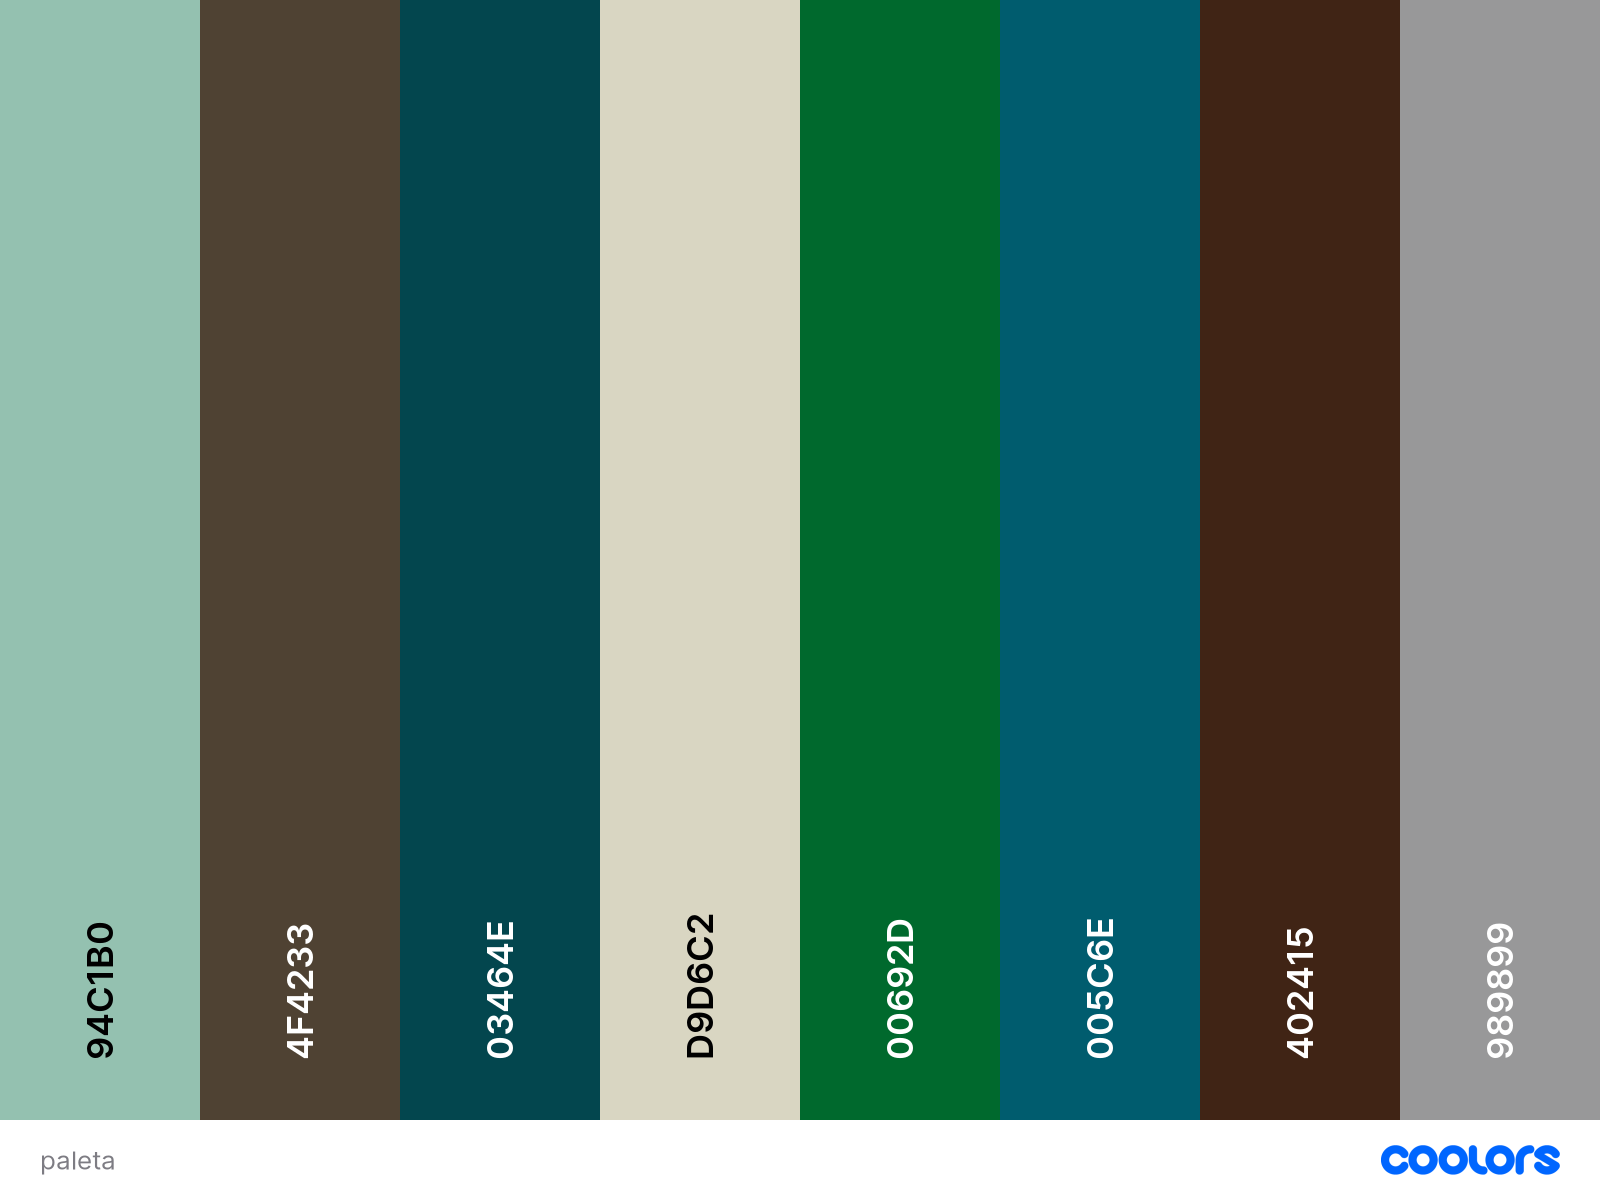
\includegraphics[width=\textwidth]{Imagenes/Fanart1/Analysis/paleta.png}
                \caption{Color Palette of the first fan art.}
            \end{figure}

            The tonality is mostly warm due to the yellowish tone of the sun and the brown of the mountains. But there's also the cold colors used on the river, Zelda and the grass.\\
            \begin{figure}[H]
                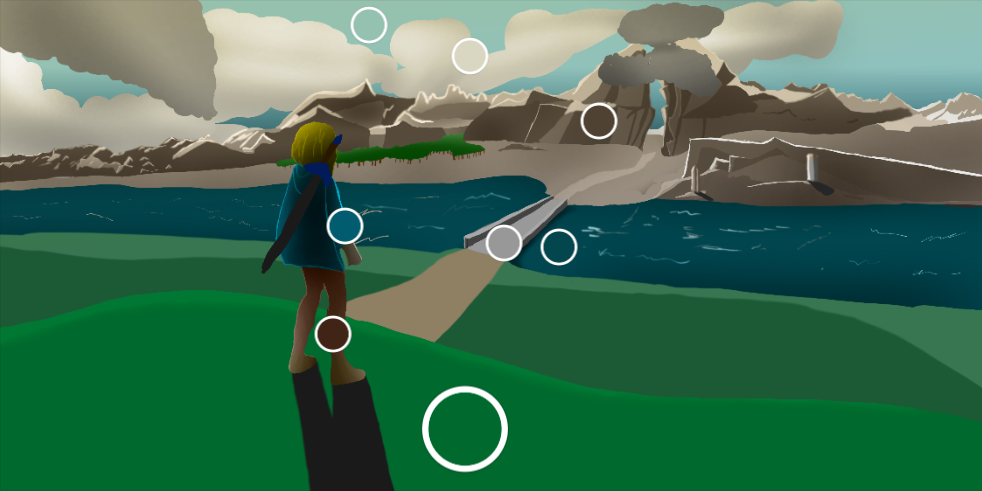
\includegraphics[width=\textwidth]{Imagenes/Fanart1/Analysis/tonalidad.png}
                \caption{Color Tonality of the first fan art.}
            \end{figure}

            The contrasts used are:
            \begin{itemize}
                \item \textbf{Tonality Contrast:} Used to differentiate the trees from the plains.
                \item \textbf{Saturation Contrast:} Used to differentiate foreground from the background mountains. 
                \item \textbf{Luminance Contrast:} Used to differentiate the difference between the sky. 
            \end{itemize}

            \begin{figure}[H]
                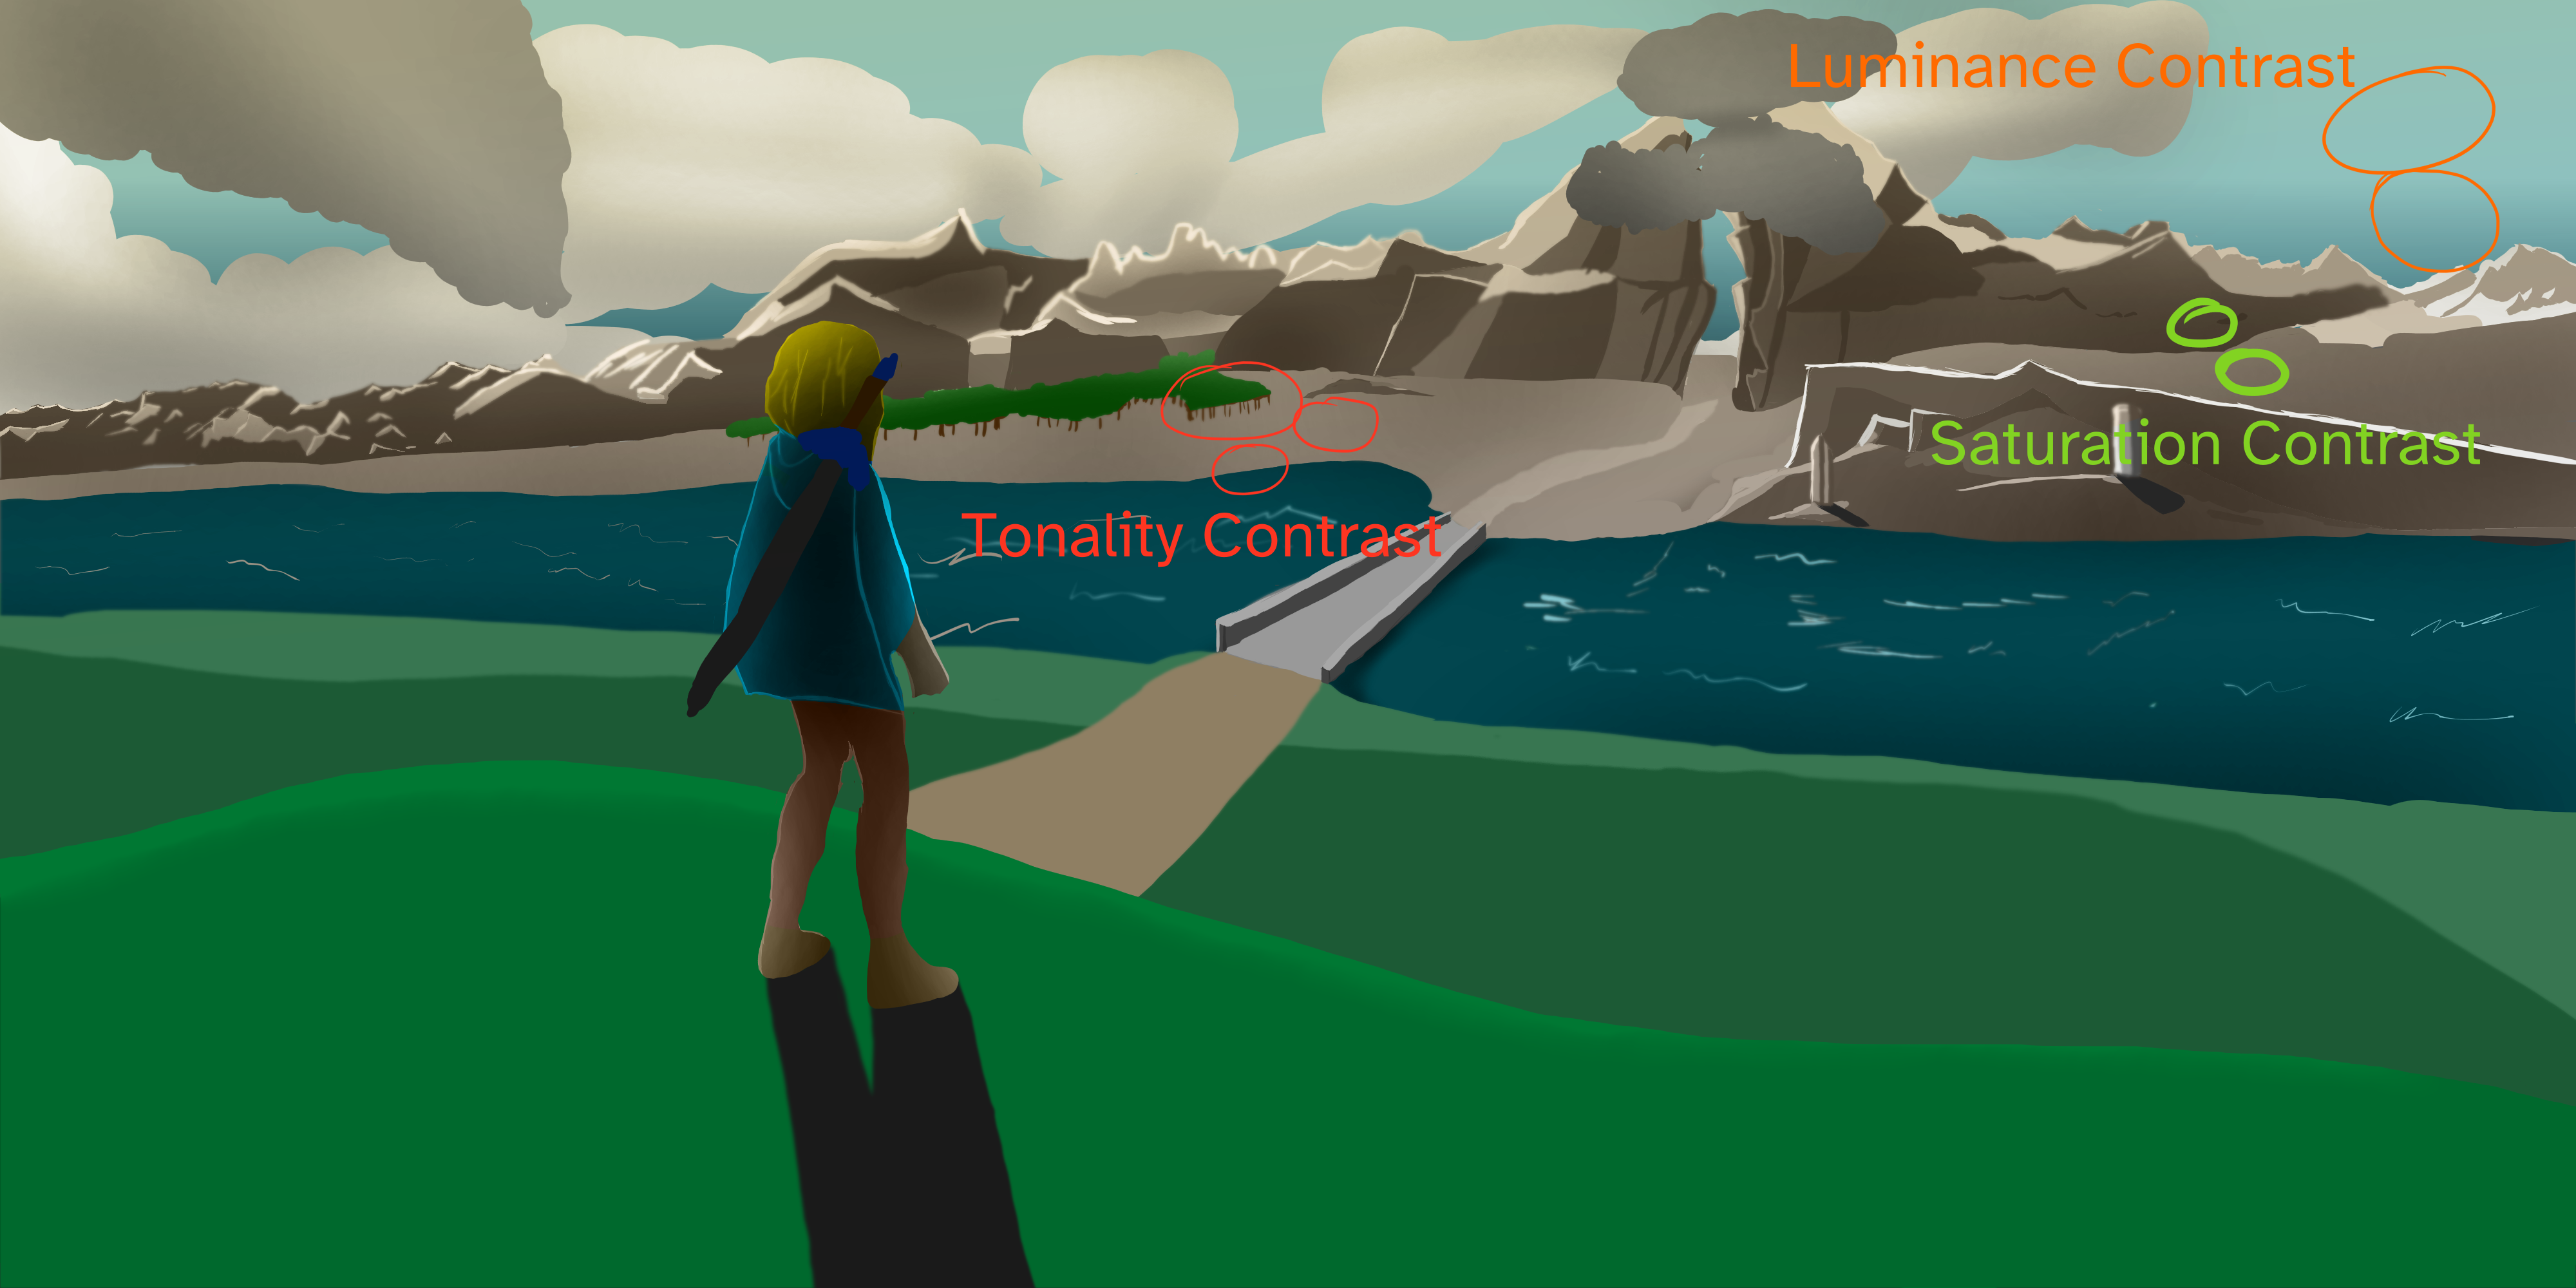
\includegraphics[width=\textwidth]{Imagenes/Fanart1/Analysis/contraste.png}
                \caption{Contrasts of the first fan art.}
            \end{figure}

\newpage
%%______________________________________________________________________________
%%______________________________________________________________________________
\newpage
\section{Second Illustration}

    \subsection{Line art and sketches}

        With the second fan art, I wanted to use my full 3D skills to use. So I used two different rigs with more detail on the posing. \\
        
        I wanted a more dynamic pose for Zelda, so I created a pose that allowed me to create as much movement with the pose as I could. The sword was also one of the main \textit{characters} of the composition because it adds the movement to the rest of the composition.\\

        Moreover, I also wanted another character in the fan art that could add a sense of danger to the image. So I decided to use a Guardian, one of the biggest roadblocks that players often face in the game.\\

        \begin{figure}[H]
            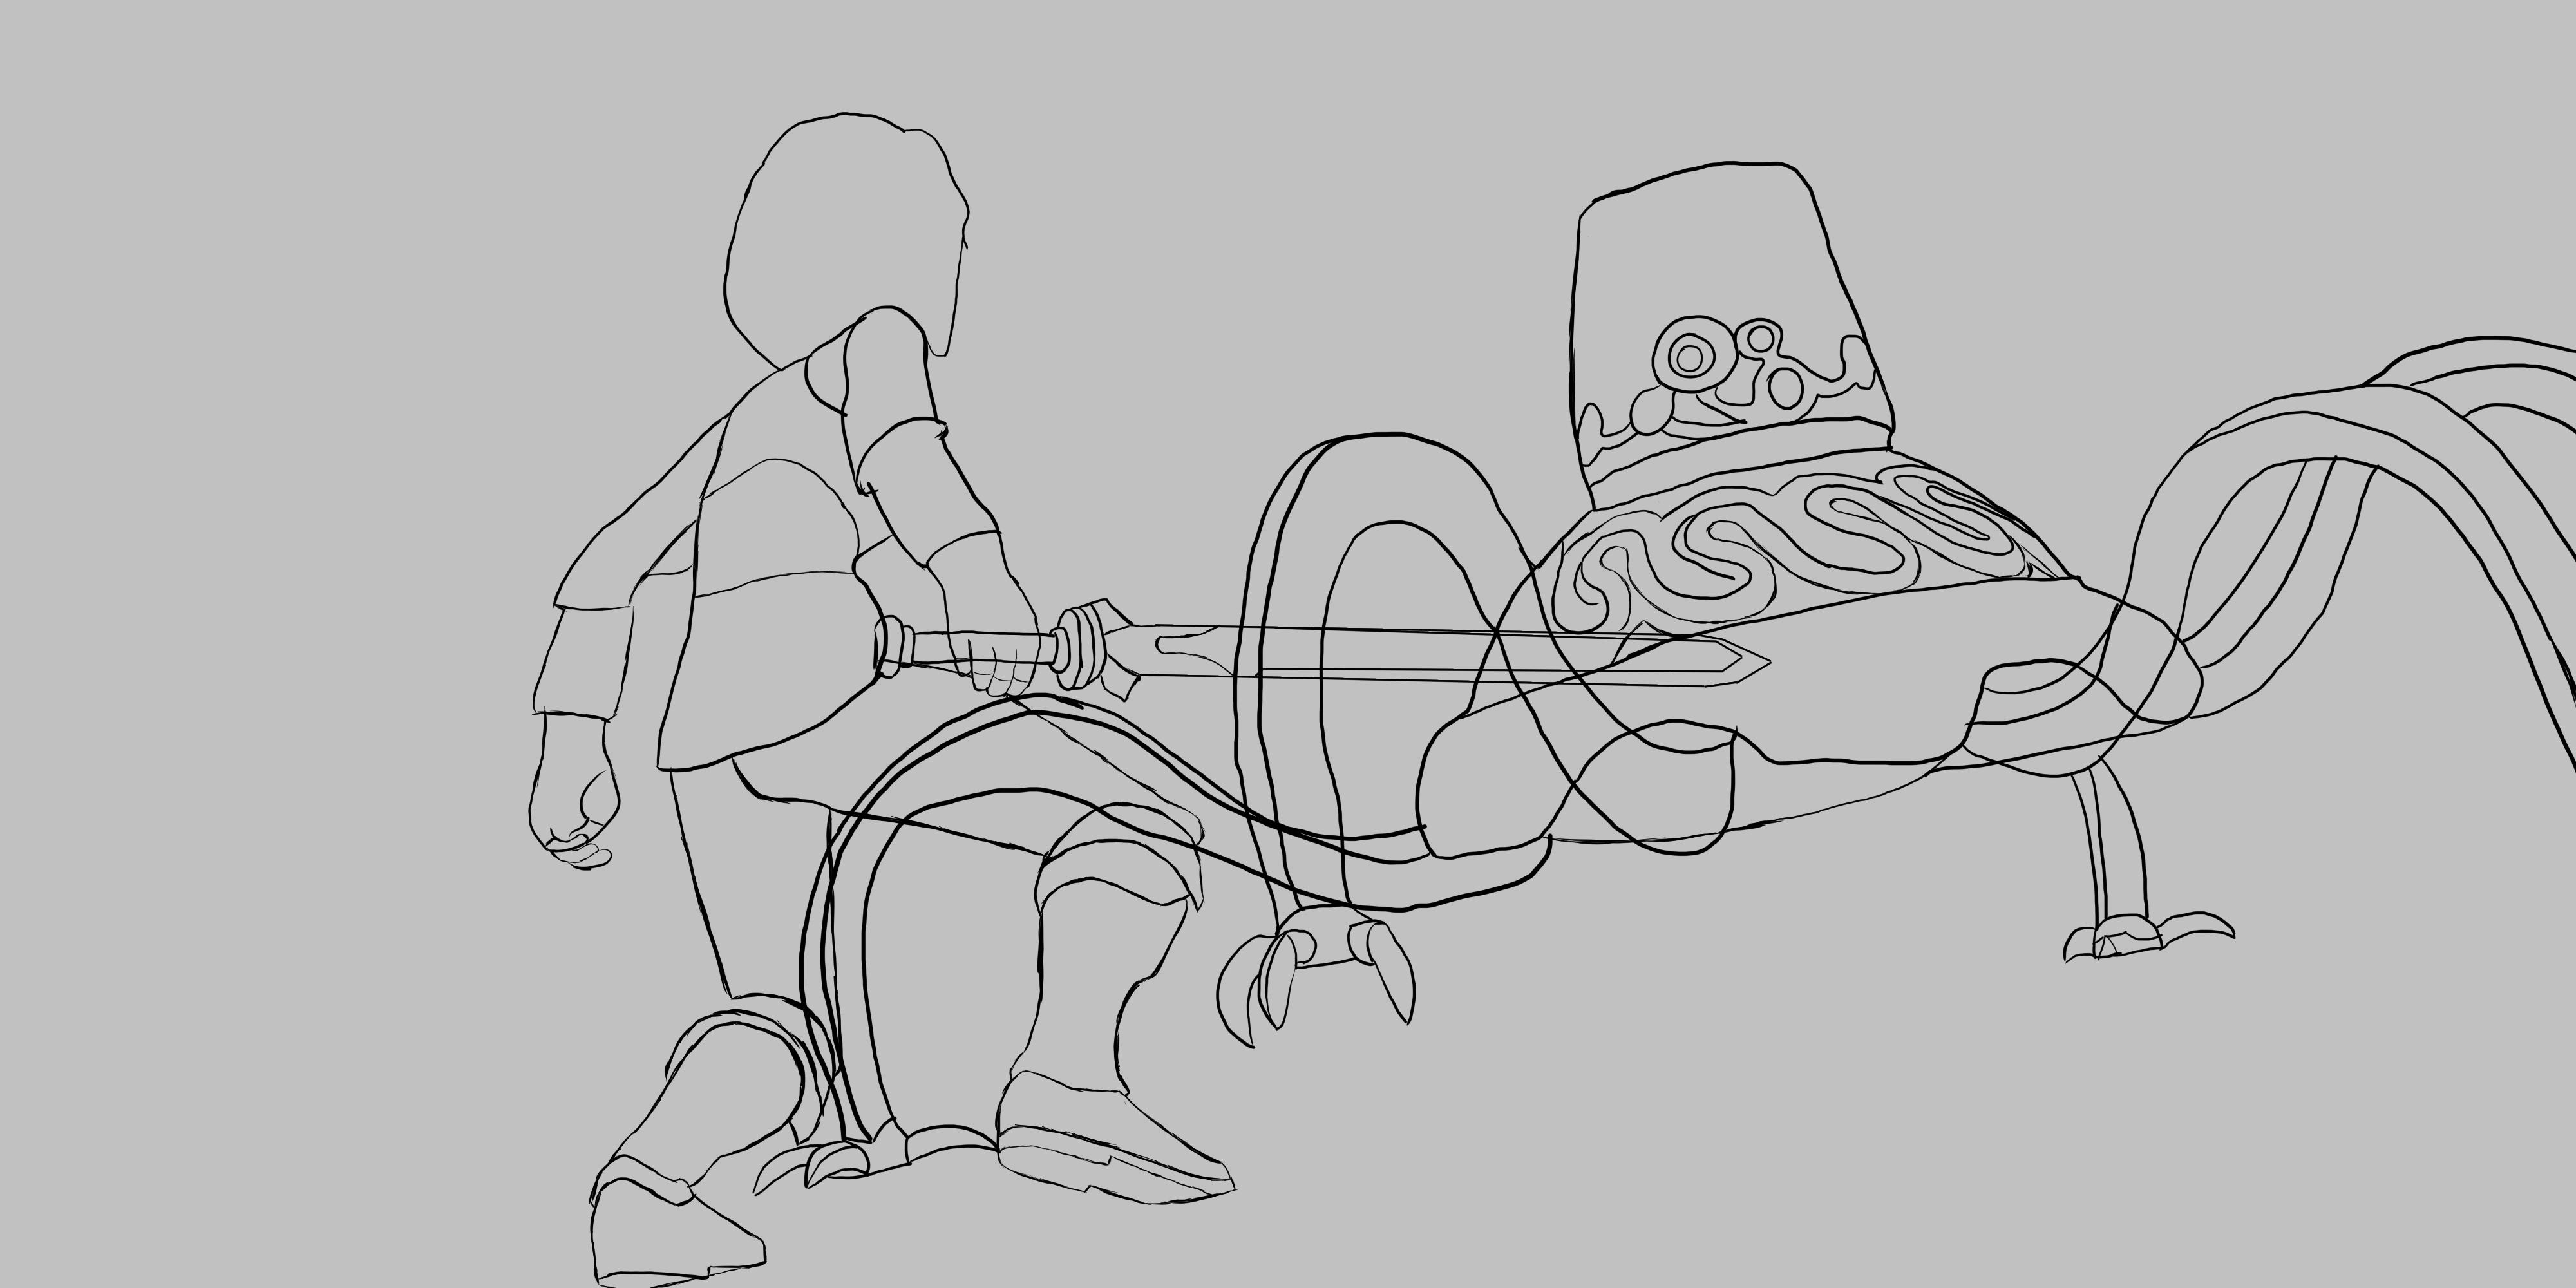
\includegraphics[width=\textwidth]{Imagenes/Fanart2/Boceto_Lineart/I Iteracion_LineArt.png}
            \caption{First iteration of the second fan art.}
        \end{figure}

        This was a basic step to add some trees.
        \begin{figure}[H]
            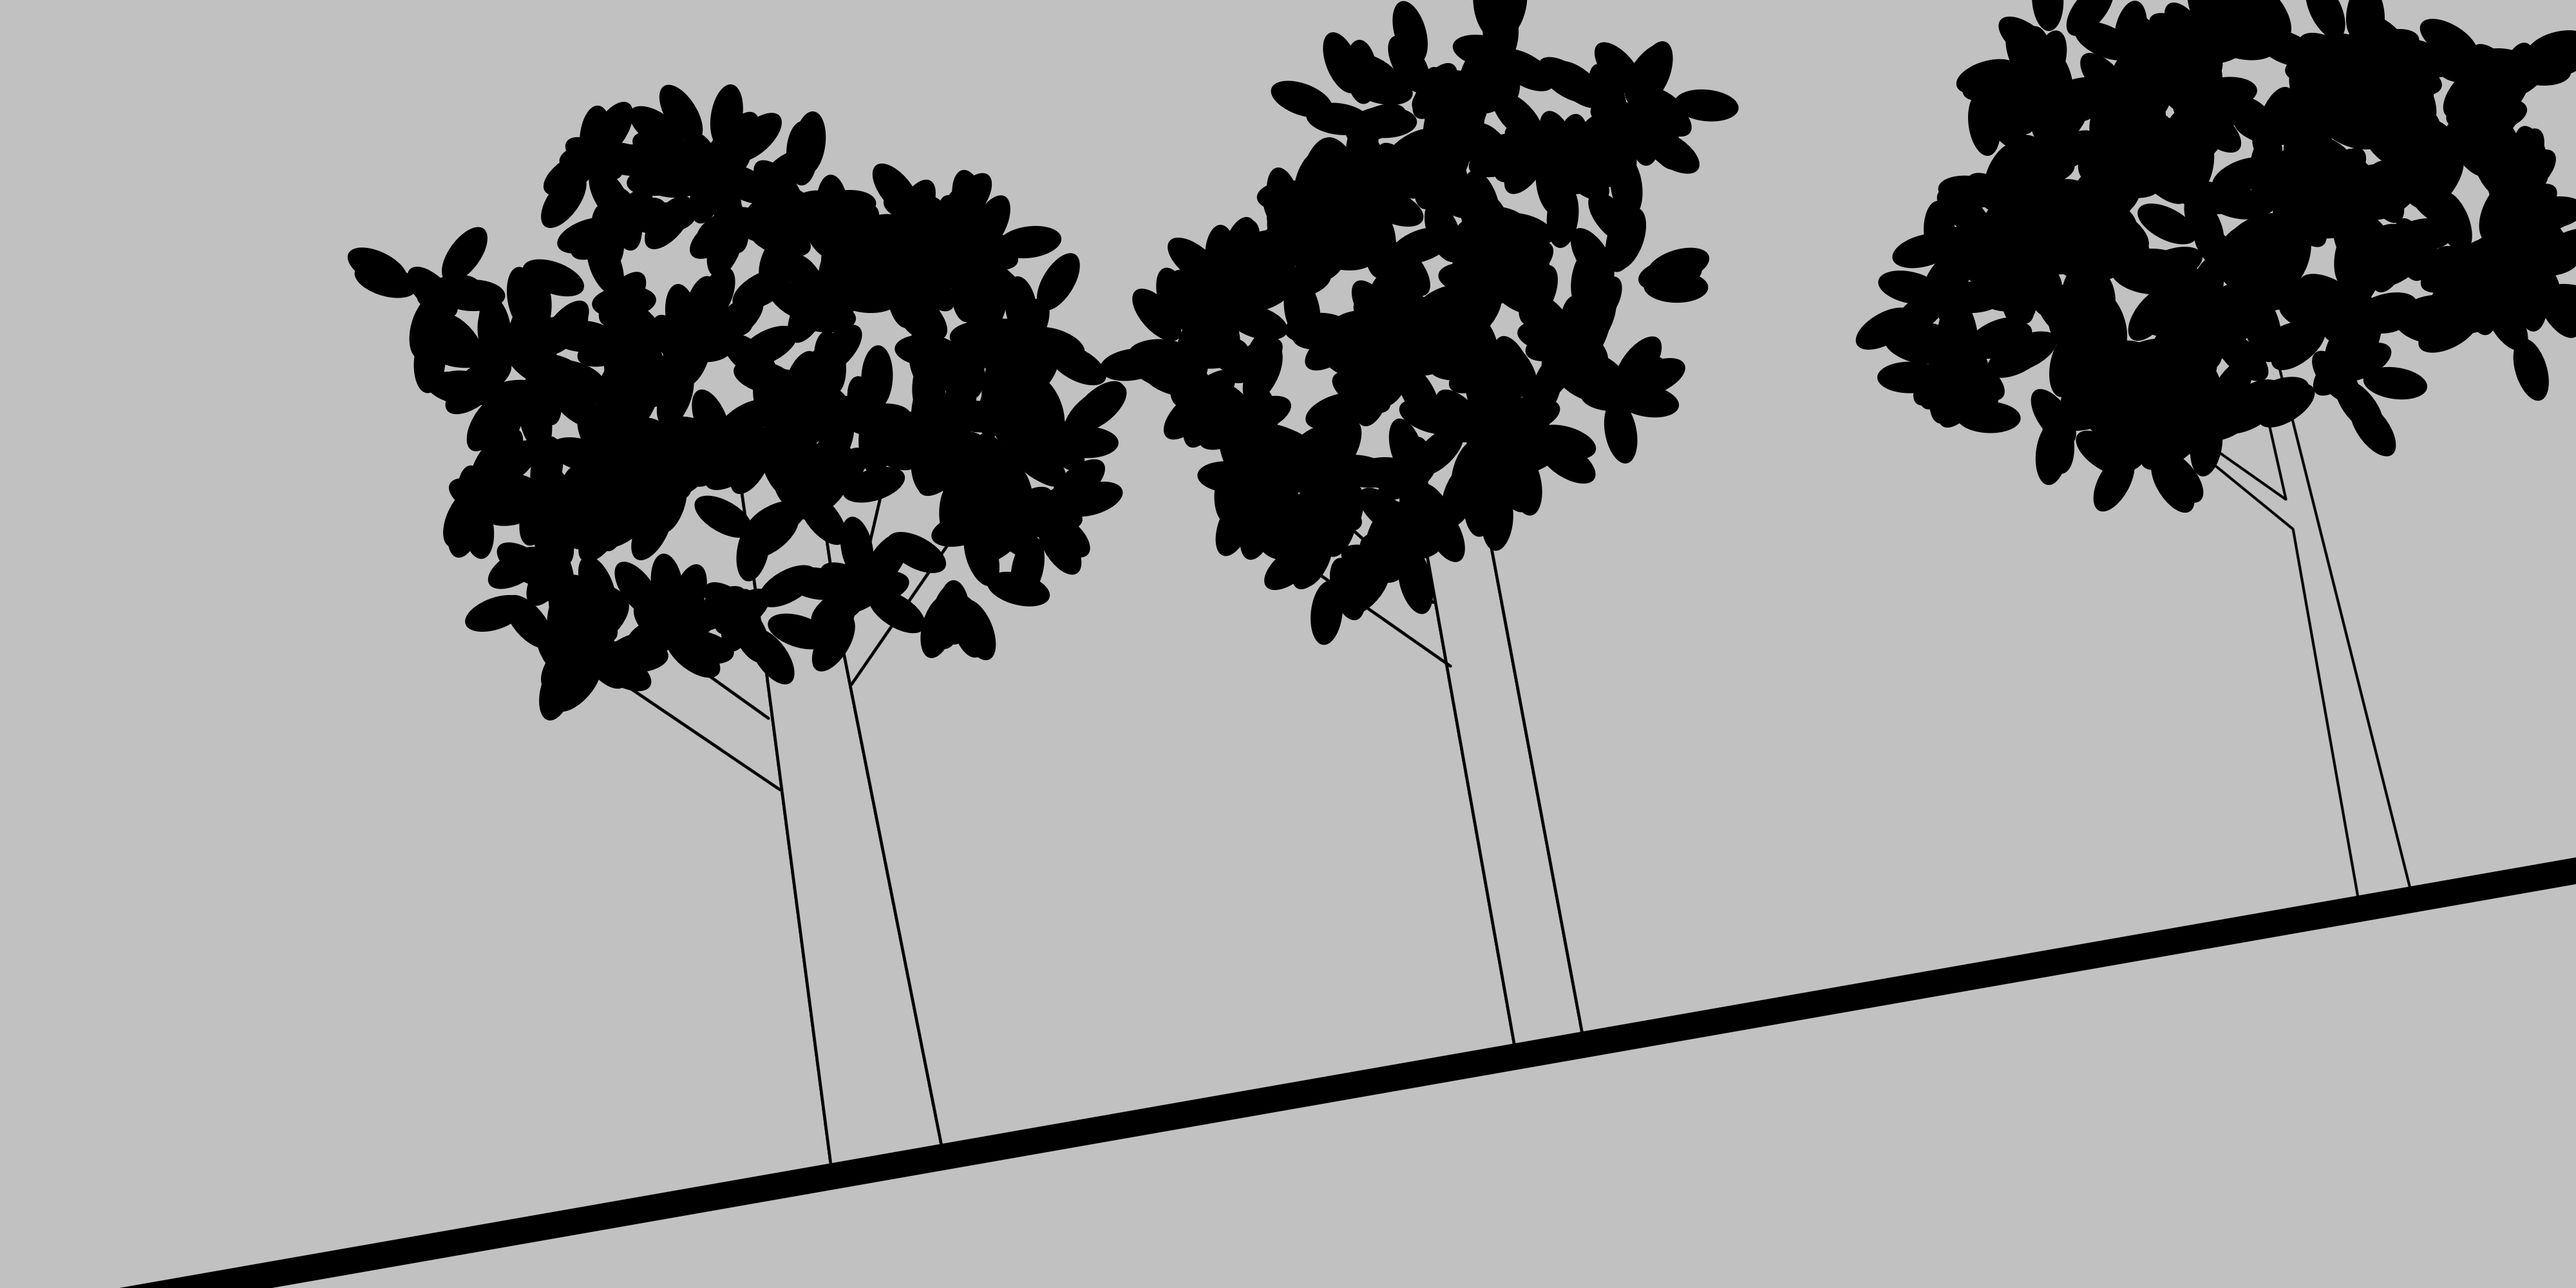
\includegraphics[width=\textwidth]{Imagenes/Fanart2/Boceto_Lineart/II Iteracion_LineArt.png}
            \caption{Second iteration of the second fan art.}
        \end{figure}

        On the third step I overlaid the trees, the Guardian, and Zelda. 
        \begin{figure}[H]
            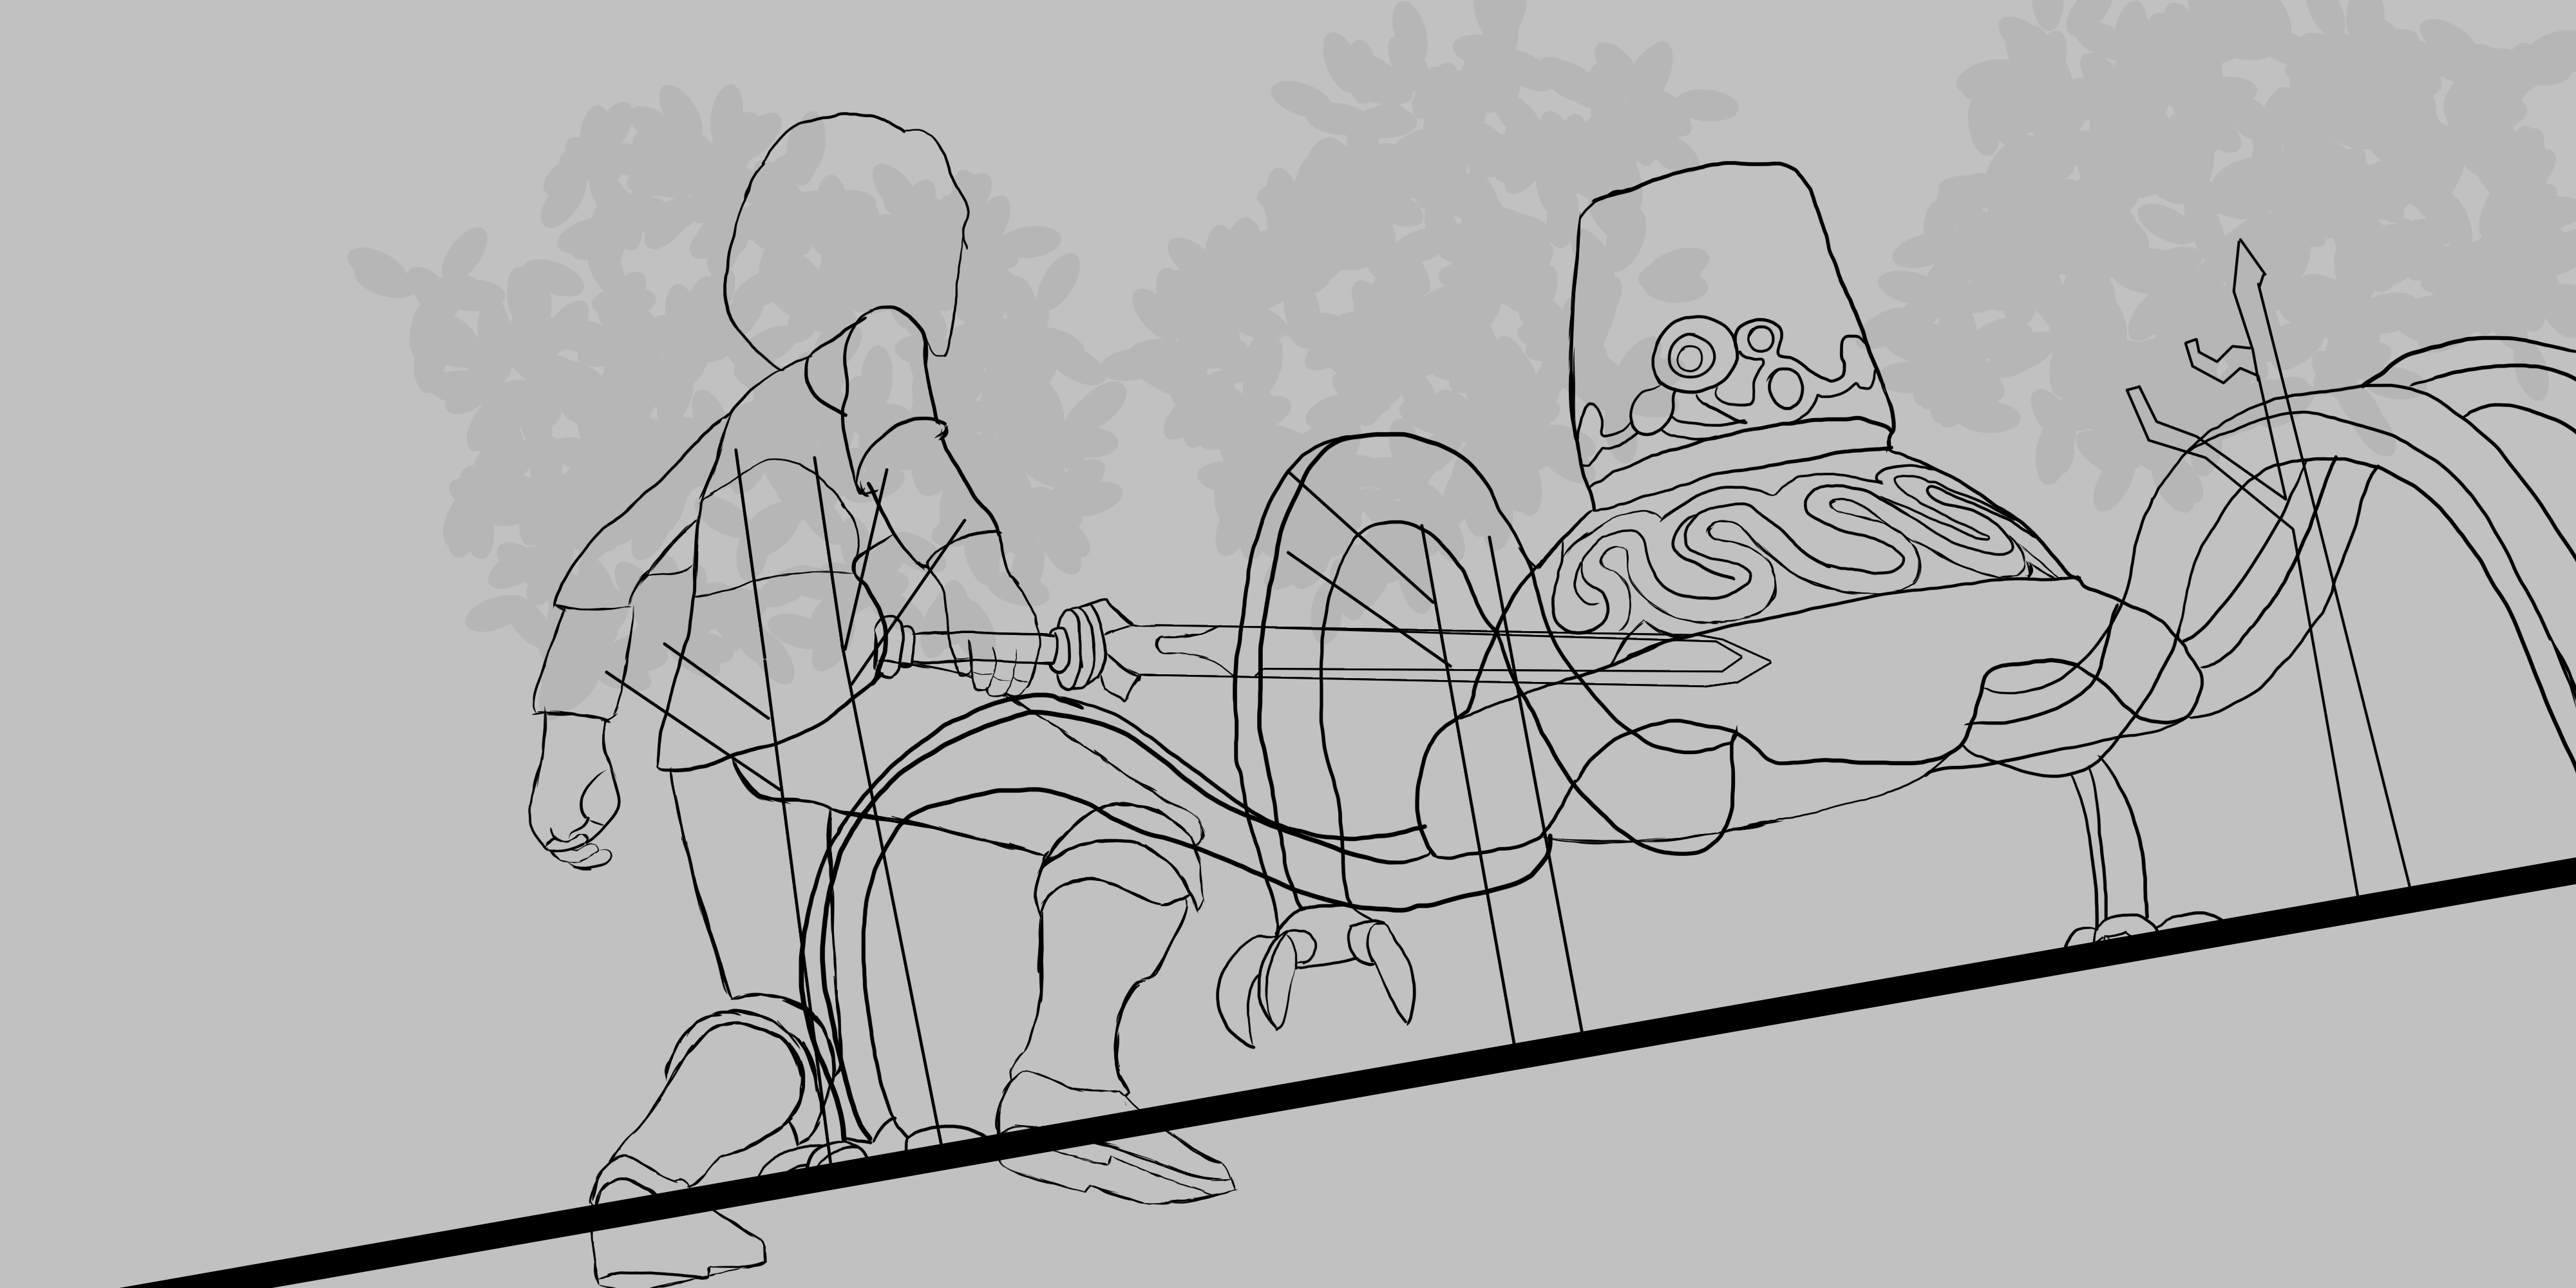
\includegraphics[width=\textwidth]{Imagenes/Fanart2/Boceto_Lineart/III Iteracion_2o_FanArt_LineArt.png}
            \caption{Third iteration of the second fan art.}
        \end{figure}

\newpage
    \subsection{Chiaroscuro}

        First, I started doing some basic shading on the chiaroscuro, with only changing the greyscale of the colors depending on how far away the subject is, except the guardian arms, which I wanted to make it stand out. 
        \begin{figure}[H]
            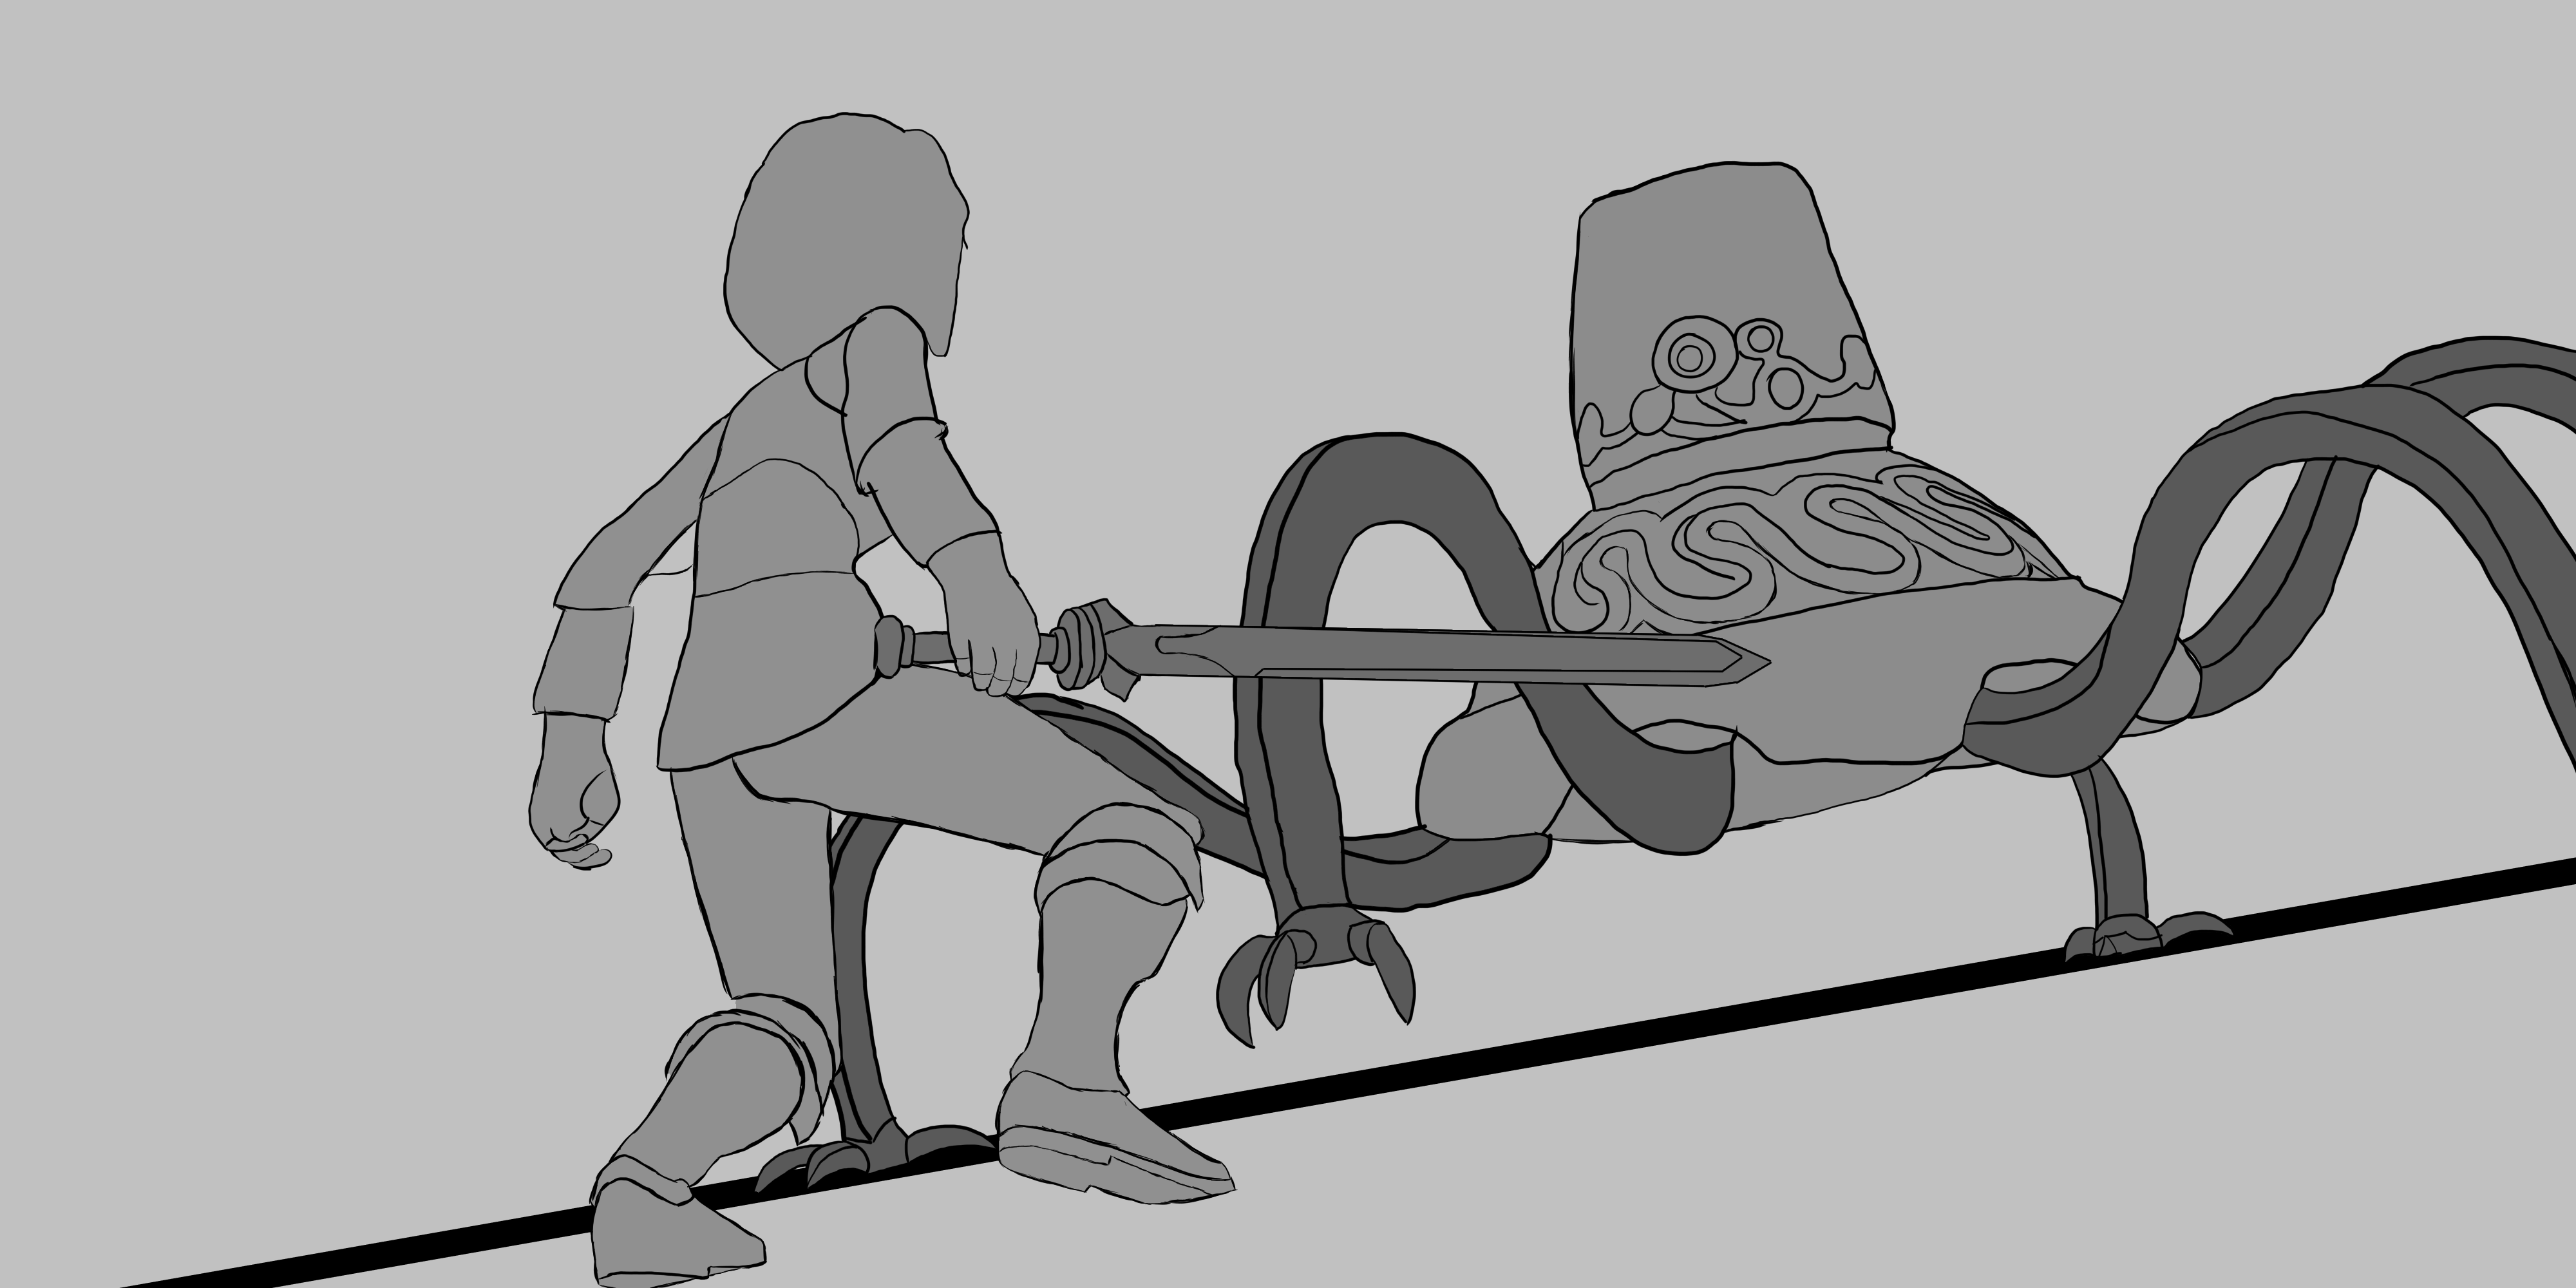
\includegraphics[width=\textwidth]{Imagenes/Fanart2/Claroscuro/I_Iteracion.png}
            \caption{Chiaroscuro of the second fan art.}
        \end{figure}

        Following with the first iteration, I added the shading having into account where the lightning will come from.
        \begin{figure}[H]
            \includegraphics[width=\textwidth]{Imagenes/Fanart2/Claroscuro/II_Iteración.png}
            \caption{Chiaroscuro of the second fan art.}
        \end{figure}

        I added the trees and made a basic shading to them to see how they would look like. 
        \begin{figure}[H]
            \includegraphics[width=\textwidth]{Imagenes/Fanart2/Claroscuro/III_Iteraion.png}
            \caption{Chiaroscuro of the second fan art.}
        \end{figure}

        At this stage I removed the line art from the models and continued to color the fan art. 
        \begin{figure}[H]
            \includegraphics[width=\textwidth]{Imagenes/Fanart2/Claroscuro/IIII_Iteracion.png}
            \caption{Chiaroscuro of the second fan art.}
        \end{figure}

\newpage
    \subsection{Coloring}
        I wanted to be as truth as possible to the source material with the coloring of this fan art. 
        
        So I extracted the colors from the 3D renders, and made a palette out of them.\\

        For the first iteration, I flat colored the fan art following the chiaroscuro and using contrast saturation to differentiate the colors.\\
        \begin{figure}[H]
            \includegraphics[width=\textwidth]{Imagenes/Fanart2/Color/I_Iteracionç.png}
            \caption{Coloring of the second fan art.}
        \end{figure}

        For the second iteration, I shaded the flat coloring and added a gradient background, but I kept the line for now.\\
        \begin{figure}[H]
            \includegraphics[width=\textwidth]{Imagenes/Fanart2/Color/II_Iteracion.png}
            \caption{Coloring of the second fan art.}
        \end{figure}

        On this step, I removed the line art and colored the trees.

        Due to a saving error with the layers, I lost the shading of the Guardian and needed to redo the shading for it.\\

        Luckily I had a previous version of the GIT repository and I could recover the PNG file, so I redid the shading.\\
        \begin{figure}[H]
            \includegraphics[width=\textwidth]{Imagenes/Fanart2/Color/III_Iteración.png}
            \caption{Coloring of the second fan art.}
        \end{figure}

        On this step, I shaded the trees and completed the shading on the Guardian.\\
        \begin{figure}[H]
            \includegraphics[width=\textwidth]{Imagenes/Fanart2/Color/IIII_Iteracion.png}
            \caption{Coloring of the second fan art.}
        \end{figure}

    \subsection{Final Result}

        \begin{figure}[H]
            \includegraphics[width=\textwidth]{Imagenes/Fanart2/Color/IIII_Iteracion.png}
            \caption{Final Result of the second fan art.}
        \end{figure}

\newpage
    \subsection{Formal elements of the image}
        
        \subsubsection{Perspective}

            The horizon line is situated at lower than the middle of the image, so we can say that this image is a low angle one.\\
            \begin{figure}[H]
                \includegraphics[width=\textwidth]{Imagenes/Fanart2/Analysis/horizonte.png}
                \caption{Horizon line of the second fan art.}
            \end{figure}

            Because this composition doesn't have any kinds of buildings nearby or artificial constructions, the image doesn't have any kind of vanishing point.\\

        \subsubsection{Composition}

            The rule of thirds is applied thoroughly in this image as most of the interest points of the image are situated on the higher left and right third of the image. So this makes the composition very balanced in terms of characters. 
            \begin{figure}[H]
                \includegraphics[width=\textwidth]{Imagenes/Fanart2/Analysis/Analysis.png}
                \caption{Rule of Thirds of the second fan art.}
            \end{figure}

            The interest points are mostly interconnected with each other because the characters are fighting each other, so there's a lot of tension between them.\\
            \begin{figure}[H]
                \includegraphics[width=\textwidth]{Imagenes/Fanart2/Analysis/puntos_interes.png}
                \caption{Interset Points of the second fan art.}
            \end{figure}

            The visual paths use Zelda to lead the eye to the Guardian, which the paths are helped by Zelda's sword, which is pointing to the Guardian.\\
            \begin{figure}[H]
                \includegraphics[width=\textwidth]{Imagenes/Fanart2/Analysis/recorridos.png}
                \caption{Visual Paths of the second fan art.}
            \end{figure}

            The image is symmetrical in terms of the characters, but because of the menacing silhouette of the Guardian, the balance of the weight on this image is difficult to analyze.\\

            Because Zelda occupies most of the left space but at the same time, the Guardian occupies most of the right space, just a bit less of it.\\

            \begin{figure}[H]
                \includegraphics[width=\textwidth]{Imagenes/Fanart2/Analysis/balanza.png}
                \caption{Weight Scaling of the second fan art.}
            \end{figure}

        \subsubsection{Chiaroscuro}

            I wanted to give a lot of priority to the chiaroscuro to this image because there are a lot of elements on this image, and if even one of them is not clearly separated from the rest, the image would look very messy and very easy to miss the point.\\
            \begin{figure}[H]
                \includegraphics[width=\textwidth]{Imagenes/Fanart2/Analysis/claroscuro.png}
                \caption{Chiaroscuro of the second fan art.}
            \end{figure}

            The pixelization makes the chiaroscuro more clear, so we can define the image as a medium key chiaroscuro. It has a lot of white areas mixed with dark hard shadows.\\
            \begin{figure}[H]
                \includegraphics[width=\textwidth]{Imagenes/Fanart2/Analysis/pixel.png}
                \caption{Pixelizated Chiaroscuro of the second fan art.}
            \end{figure}

            The light comes from the right part of the image, covering the image with a tenuous white light which is also slightly angled from the origin point. 
            \begin{figure}[H]
                \includegraphics[width=\textwidth]{Imagenes/Fanart2/Analysis/recorrido luz.png}
                \caption{Light Paths of the second fan art.}
            \end{figure}

        \subsubsection{Color}

            The color palette used is very varied, ranging from warm colors of the Guardian to the cold and hard colors used within Zelda and the background.

            \begin{figure}[H]
                \includegraphics[width=\textwidth]{Imagenes/Fanart2/Analysis/palette.png}
                \caption{Color Palette of the second fan art.}
            \end{figure}

            The tonality on these images varies widely with what the spectator is seeing. \\
            The Guardian has a very warm color palette thanks to its golden riveting and the pink lights emanating from it, also due to its golden claws. \\
            Meanwhile, Zelda has a colder color palette, with some browns sprinkled it to add some difference to her clothes. \\
            \begin{figure}[H]
                \includegraphics[width=\textwidth]{Imagenes/Fanart2/Analysis/tonalidad.png}
                \caption{Color Tonality of the second fan art.}
            \end{figure}

            Contrast between colors is used extensively on this image to separate everything between planes, because there three main subjects in the composition.
            The contrasts used are:
            \begin{itemize}
                \item \textbf{Luminance contrast:} Which is used on Zelda's clothes to differentiate the more lighten up areas of the clothes. 
                \item \textbf{Saturated contrast:} Is used on the leaves to separate the dark areas of the tree with the more whitened ones.
                \item \textbf{Tonality contrast:} Is used on the Guardian to separate its pink lights with the riveting ornamenting its robotic body.  
            \end{itemize}
            \begin{figure}[H]
                \includegraphics[width=\textwidth]{Imagenes/Fanart2/Analysis/contraste.png}
                \caption{Contrasts of the second fan art.}
            \end{figure}

\newpage
%%______________________________________________________________________________
%%______________________________________________________________________________
\newpage
\section{Third Illustration}
For the third fan art, I wanted to recreate the scene from the last cinematic of the game. I choose the moment where Zelda is talking to Link and there's a landscape behind her, but also her being one of the main focuses of the shot.\\

I decided to use my 3D Zelda Rig one more and change her pose a bit to make it a bit more dynamic, in addition to using the original background from the shot.\\

    \subsection{Line art and sketches}
        I commenced drawing the sketch of how the background should like, with the wavy lines representing where Zelda should go. 
        \begin{figure}[H]
            \includegraphics[width=\textwidth]{Fanart3/1_LineArt/I_Iteracion.png}
            \caption{First Iteration of the Line Art of the third fan art.}
        \end{figure}

        Then I drew Zelda, with a lot of details. I did it like this because this is an important moment of the game and wanted to try to represent as much expression as I possibly could. 
        \begin{figure}[H]
            \includegraphics[width=\textwidth]{Fanart3/1_LineArt/II_Iteracion.png}
            \caption{Second Iteration of the Line Art of the third fan art.}
        \end{figure}

        On this iteration I merged both foreground where Zelda is located and the background.
        \begin{figure}[H]
            \includegraphics[width=\textwidth]{Fanart3/1_LineArt/III_Iteracion.png}
            \caption{Third Iteration of the Line Art of the third fan art.}
        \end{figure}

    \subsection{Chiaroscuro}

        On the first iteration of the chiaroscuro I separated everything on the background by different scales on gray, provided by Krita's default color palette. 
        \begin{figure}[H]
            \includegraphics[width=\textwidth]{Fanart3/2_Claroscuro/I_Iteracion.png}
            \caption{First Iteration of the Chiaroscuro of the third fan art.}
        \end{figure}

        After that I added the chiaroscuro on Zelda, trying to analyze and make sense of how the light would reflect on her clothes.\\

        Because of the importance on light on this fan art, I tried to make it as accurate as possible as the cinematic shot of the game. So I took the light references from the cinematic and applied it to the fan art.\\

        Also, I tried to replicate the cel-shading aspect of the shadows by making them hard. 
        \begin{figure}[H]
            \includegraphics[width=\textwidth]{Fanart3/2_Claroscuro/II_Iteracion.png}
            \caption{Second Iteration of the Chiaroscuro of the third fan art.}
        \end{figure}

        On this iteration I added a few more details to the illumination on the background.
        \begin{figure}[H]
            \includegraphics[width=\textwidth]{Fanart3/2_Claroscuro/III_Iteracion.png}
            \caption{Third Iteration of the Chiaroscuro of the third fan art.}
        \end{figure}

        I removed the lines on this iteration and fixed the eyes on Zelda, because at this step I haven't considered the chiaroscuro without lines yet.\\ 
        So in some parts, Zelda doesn't have any kind of contrasts with the backgrounds and seems like it's \textit{at the same level of depth}.
        \begin{figure}[H]
            \includegraphics[width=\textwidth]{Fanart3/2_Claroscuro/IIII_Claroscuro.png}
            \caption{Fourth Iteration of the Chiaroscuro of the third fan art.}
        \end{figure}

        After learning what I had seen on the previous interactions, I fixed Zelda's shading by modifying some greys, so she could be separated from the background much better, creating a foreground just for her.
        \begin{figure}[H]
            \includegraphics[width=\textwidth]{Fanart3/2_Claroscuro/IIIII_Claroscuro.png}
        \end{figure}

    \subsection{Coloring}

        I started the coloring with the background by creating some simple flat coloring with taking into account the lightning conditions that I set beforehand. 
        \begin{figure}[H]
            \includegraphics[width=\textwidth]{Fanart3/3_Color/I_Color.png}
            \caption{First Iteration of the Coloring of the third fan art.}
        \end{figure}

        After finishing up the background, I added colors to Zelda in the same manner as the background. Doing the flat colors and then adding the shadow similarly on how the shadows are processed in the game, with the cel-shading styling. 
        \begin{figure}[H]
            \includegraphics[width=\textwidth]{Fanart3/3_Color/II_Color.png}
            \caption{Second Iteration of the Coloring of the third fan art.}
        \end{figure}

        I removed the line on this iteration, but I forgot to color some parts of the drawing that were obfuscated by the lines. So I fixed it on the next iteration.
        \begin{figure}[H]
            \includegraphics[width=\textwidth]{Fanart3/3_Color/III_Color.png}
            \caption{Third Iteration of the Coloring of the third fan art.}
        \end{figure}

        On the fourth iteration of this fan art, I fixed the lines previously mentioned.\\
        I added some gradients to the borders of the foreground and background to separate them a little more.\\
        \begin{figure}[H]
            \includegraphics[width=\textwidth]{Fanart3/3_Color/IIII_Color.png}
            \caption{Fourth Iteration of the Coloring of the third fan art.}
        \end{figure}

        For the final iteration, I added fixed some shading that looked weird or out of place and polished the shading on Zelda, specially around the right arm and the chest, which looked very flat on the previous iteration. 
        \begin{figure}[H]
            \includegraphics[width=\textwidth]{Fanart3/3_Color/IIIII_Color.png}
        \end{figure}

    \subsection{Final Result}

        \begin{figure}[H]
            \includegraphics[width=\textwidth]{Fanart3/3_Color/IIIII_Color.png}
             \caption{Final Result of the third fan art.}
         \end{figure}

    \subsection{Formal elements of the image}

        \subsubsection{Perspective}
            The horizon line situated almost at the center of the image, making it an eye level camera angle. 
            \begin{figure}[H]
                \includegraphics[width=\textwidth]{Fanart3/0_Analisi/horizonte.png}
                \caption{Perspective of the third fan art.}
            \end{figure}

            There's a vanishing point, almost at the center of the image. The paths marked in red shows where the perspective is headed at. 
            \begin{figure}[H]
                \includegraphics[width=\textwidth]{Fanart3/0_Analisi/puntofuga.png}
                \caption{Vanishing Point of the third fan art.}
            \end{figure}

        \subsubsection{Composition}

            The rule of thirds is used on this image to position Zelda at both left thirds of the image, creating a composition where the main focus is Zelda.\\
            This was also made to follow the original cutscene format, where Zelda is also positioned at the same side. 
            \begin{figure}[H]
                \includegraphics[width=\textwidth]{Fanart3/0_Analisi/tercios.png}
                \caption{Composition of the third fan art.}
            \end{figure}

            The points of interest begin at Zelda, more specifically, at her eyes where the intense teal colored eyes contrast with her skin, making it emphasize her face.\\
            The spectator will inspect Zelda and then progress to analyze the rest of the background, starting with the rock in the middle and the mountains at the back. \\
            \begin{figure}[H]
                \includegraphics[width=\textwidth]{Fanart3/0_Analisi/puntosinteres.png}
                \caption{Interest Points of the third fan art.}
            \end{figure}

            The paths that the image cover, are mostly done with the eyes of Zelda, making a line where she's looking.\\
            Also, the \textit{wavy} form of the environment contribute to the paths. 
            \begin{figure}[H]
                \includegraphics[width=\textwidth]{Fanart3/0_Analisi/recorridos.png}
                \caption{Lines of the third fan art.}
            \end{figure}

            The wight balance on this image is very uncompensated. Zelda takes a lot of the composition, and the coloring and presence that she makes, obfuscates the rest of the composition.\\
            Making the left side of the image very heavy. 
            \begin{figure}[H]
                \includegraphics[width=\textwidth]{Fanart3/0_Analisi/balanza.png}
                \caption{Space of the third fan art.}
            \end{figure}

        \subsubsection{Chiaroscuro}

            The chiaroscuro on this image is really important due to the necessity of separating Zelda, from the rest of the composition.
            \begin{figure}[H]
                \includegraphics[width=\textwidth]{Fanart3/0_Analisi/claroscuro.png}
                \caption{Chiaroscuro of the third fan art.}
            \end{figure}

            If we pixelize the chiaroscuro, we can see the heavy emphasis on white colors on the composition, making it a very high key image, with some touches of darker colors. 
            \begin{figure}[H]
                \includegraphics[width=\textwidth]{Fanart3/0_Analisi/pixelize.png}
                \caption{Pixelizated Chiaroscuro of the third fan art.}
            \end{figure}

            The light comes from an unknown place, but at the same time we know it's coming from the left a bit low from the middle. 
            \begin{figure}[H]
                \includegraphics[width=\textwidth]{Fanart3/0_Analisi/light path.png}
                \caption{Light Paths of the third fan art.}
            \end{figure}

        \subsubsection{Color}
            
            The color palette of the image says out loud that it has a lot of colors.\\
            Zelda uses blue, brownish red and white on her clothes and bright yellow on her hair, making a dominant presence on the composition color wise.\\
            While in the background the mountains with the coffee brown color shines where it needs to and the green hills contribute to the separating Zelda from the background. \\
            \begin{figure}[H]
                \includegraphics[width=\textwidth]{Fanart3/0_Analisi/paleta.png}
                \caption{Color palette of the third fan art.}
            \end{figure}

            The tonality of the image is cold in general, only being interrupted by the brown at the background with the mountains.\\
            Using mainly blues, greens and teal, creates a very cold composition color wise. 
            \begin{figure}[H]
                \includegraphics[width=\textwidth]{Fanart3/0_Analisi/tonality.png}
                \caption{Tonality of the third fan art.}
            \end{figure}

            The contrast is used to balance the components in the composition, so there were a lot of emphasis put on the contrast on the image.\\
            \begin{itemize}
                \item \textbf{Saturation contrast:} is used on the grass to differentiate between how far away the grass is from the \textit{camera / spectator}.
                \item \textbf{Luminance contrast: } is used on the sky to differentiate the changes on whites at the sky. 
                \item \textbf{Tonality contrast: } is used on Zelda, on most of the clothes. However, the most important one is the difference of tone between the eye color and her skin color. 
            \end{itemize}
            \begin{figure}[H]
                \includegraphics[width=\textwidth]{Fanart3/0_Analisi/contrast.png}
                \caption{Contrast of the third fan art.}
            \end{figure}



    \newpage
%%______________________________________________________________________________
%%______________________________________________________________________________
\newpage
\section{Extra Section}
\begin{multicols}{2}

\textbf{Esta sección será escrita en castellano y en inglés, debido a que es una sección dedicada a hablar del formato del documento, no obstante, también estará escrita en inglés más adelante.\\}

\columnbreak

\textbf{This section will be written in English and Spanish, due to this section is dedicated to talk about the format of the document, however, it will be written in Spanish later.\\}
\end{multicols}

\subsection{English}
On this extra section, I want to talk about the decisions regarding other elements that compose this document. 
For the template I used the 
\href{https://www.overleaf.com/latex/templates/pan-template-for-submission-to-political-analysis/csxqmspqzntv}{PAN - Template for submission to Political Analysis} because the template offered a good balance of clear text presentation, and because it's a wide template images look good when they are adjusted by using:
\begin{verbatim} 
    width=\textwidth 
\end{verbatim}

For the fonts used on the document, the font is 
\href{https://brailleinstitute.org/freefont}{Atkinson Hyperlegible}.\\
It's a font that was designed to be used by people with visual disabilities, so it offers an excellent balance of stylized and readability.\\

\subsection{Castellano}

En esta sección, quiero comentar algunos aspectos  formales del documento.
Para la plantilla usé el \href{https://www.overleaf.com/latex/templates/pan-template-for-submission-to-political-analysis/csxqmspqzntv}{PAN - Template for submission to Political Analysis} debido a que esta plantilla ofrecía un buen balance de estilización combinado con una presentación de texto clara, y porque es una plantilla amplia, las imágenes se ven bien cuando se ajustan usando:

\begin{verbatim} 
    width=\textwidth 
\end{verbatim}

Para las fuentes usadas en el documento, la fuente es \href{https://brailleinstitute.org/freefont}{Atkinson Hyperlegible}.\\
Es una fuente que fue diseñada para ser usada por personas con discapacidades visuales, por lo que ofrece un excelente balance de estilización y legibilidad.\\

\newpage
\section{Conclusions}

Concluding with the document, I can say that this has been a really tough work to do.\\ 

My knowledge about painting, color theory and composition were put to the test, which, in my opinion, I think I could have done better with a little more time.\\

Still, in a more critical aspect about this coursework, I think the quantity of the work that needed to be done, was too much with the time we had. I think that the work could have been done better if we had more time to do it.\\

However, I think the idea of combining the three subjects to do a one big project is good, and should be done more often.\\

And finally, I want to talk about my own art. I think there's a lot of improvement to be had because there are aspects on the drawings that are good enough, but others are very bland / weak.\\

But in conclusion, I can say that this has been a good experience, and I hope to do more of this kind of work in the future.\\

\newpage

\end{document}